%KECReportFormat.tex
%%%%%%%%%%%%%%%%%%%%%%%%%%%%%%%%%%%%%%%%%%%%%%%%%%%%%%%%%%%%%%%%%%%%%%%%%%%
%DO NOT MAKE CHANGES IN THIS FILE

\documentclass[12pt, a4paper]{report}
\usepackage[left = 1.5in, right = 1in, top = 1in, bottom = 1in]{geometry}%for margin
\usepackage{amsfonts, amsmath, amssymb} %for mathematical equations
\usepackage{graphicx} %for images
\usepackage{times} %font Times New Roman Font
\usepackage{float} %required if you use H(strictly here) position for floats
\usepackage[skip = 8pt,tableposition=top, figureposition=bottom]{caption}%adjust spacing of captions and specify where captions are
\usepackage{hyperref} % for easy Navigation in document, also puts links in TOC, LOF, LOT...
\usepackage{setspace} %to change line spacing in some portion \singlespacing \onehalfspacing \doublespacing
\usepackage{acro} %for List of Abbrreviation and Symbol
\acsetup{first-style = short} % set to display only short form on the command \ac{}

%packages required for complex tables
\usepackage{bigstrut} 
\usepackage{multirow}

\renewcommand{\contentsname}{Table of Contents} %Change TOC Heading ... default is "Contents" 

\parindent 0pt	%removes the indent in paragraph
\setlength{\parskip}{18pt}	%for paragraph spacing
\renewcommand{\baselinestretch}{1.5}   %Line Spacing = 1.5 line-spaces

%to reduce spacing in sections
\usepackage{titlesec}
\titlespacing*{\section}{0pt}{0pt}{0pt} %left, top, bottom spacings
\titlespacing*{\subsection}{0pt}{0pt}{0pt}
\titlespacing*{\subsubsection}{0pt}{0pt}{0pt}
\titlespacing*{\paragraph}{0pt}{0pt}{0pt}
\titlespacing*{\subparagraph}{0pt}{0pt}{0pt}

%adjust fontsizes\ of sections
\titleformat*{\section}{\fontsize{14pt}{18pt}\bfseries}
\titleformat*{\subsection}{\fontsize{13pt}{18pt}\bfseries}
\titleformat*{\subsubsection}{\fontsize{12pt}{18pt}\bfseries}
\titleformat*{\paragraph}{\fontsize{12pt}{18pt}\bfseries}
\titleformat*{\subparagraph}{\fontsize{12pt}{18pt}\bfseries}

%to reduce separation between points in list
\usepackage{enumitem}
\setlist[enumerate]{nosep} % no separation between items in enumerate
\setlist[itemize]{nosep} % no separation between items in itemize
%use \vspace{-18pt} before list to reduce paragraph spacing between list and preceeding paragraph.

%Changes for Chapter Heading Spacing and formats for numbered chapters
\makeatletter
\def\@makechapterhead#1{%
  %\vspace*{50pt}%
  {  \MakeUppercase{\ifnum \c@secnumdepth >\m@ne
        \fontsize{16pt}{1}\bfseries \@chapapp \space \thechapter\vspace{5pt}\\
    \fi
    \interlinepenalty\@M
     \bfseries #1}\par\nobreak
    %\vskip 0pt
  }}
\makeatother

%%%%%%%%%%%%%%%%%%%%%%%%%%%%%%%%%%%%%%%%%%%%%%%%%%%%%%%%%%%
%to adjust Heading spacings and fonts For unnumbered chapters, TOC, LOF ...
\makeatletter
% Redefine the \chapter* header macro to remove vertical space
\def\@makeschapterhead#1{%
  %\vspace*{50\p@}% Remove the vertical space
  {\newpage \parindent \z@ \raggedright
    \normalfont
    \interlinepenalty\@M
    \center \fontsize{16pt}{1} \bfseries \MakeUppercase{#1}\par\nobreak
    %\vskip 18\p@ % adjust space after heading 18pt
  }}
\makeatother 
%%%%%%%%%%%%%%%%%%%%%%%%%%%%%%%%%%%%%%%%%%%%%%%%%%%%%%%%%%%

%%%%%%%%%%%%%%%%%%%%%%%%%%%%%%%%%%%%%%%%%%%%%%%%%%%%%%%%%%%%%%%%%%%%%%%%%%%
% newcommand for generating Cover Page
\newcommand{\KECcoverpage}
{
\begin{titlepage}
\begin{center}
\Large{\textbf{KANTIPUR ENGINEERING COLLEGE}}\\
\large{\textbf{(Affiliated to Tribhuvan University)}}\\
\large{\textbf{Dhapakhel, Lalitpur}}\\
\vfill	%vertically fill the space 
\begin{figure}[h] % h: put logo "here"
\begin{center}

\includegraphics[width=25mm, height = 25mm]{images/logo.png}
\end{center}
\end{figure}

\large{\textbf{[Subject Code: \subCode]}}\\ %Change This Line
\large{\textbf{A \MakeUppercase{\project} \MakeUppercase{\doc} ON}}\\ %Change This Line
\Large{\textbf{\MakeUppercase{\projectTitle}}}\\

\vfill	%vertically fill the space 
\large{\textbf{Submitted by:}}\\
\large{\textbf{\submittedBy}}\\
\vfill	%vertically fill the space 
\textbf{A \MakeUppercase{\project} SUBMITTED IN PARTIAL FULFILLMENT OF THE REQUIREMENT FOR THE DEGREE OF \MakeUppercase{\degree}}\\

\vfill	%vertically fill the space 
\large{\textbf{Submitted to:}}\\
\large{\textbf{\submittedTo}}\\
\vfill
\large{\textbf{\defMonth, \defYear}}
\pagebreak
\end{center}
\end{titlepage}
}
%%%%%%%%%%%%%%%%%%%%%%%%%%%%%%%%%%%%%%%%%%%%%%%%%%%%%%%%%%%%%%%%%%%%%%%
% newcommand for generating Cover Page
%Title Page
\newcommand{\KECtitlepage}
{
\begin{titlepage}
\begin{center}
\Large{\textbf{\MakeUppercase{\projectTitle}}}\\

\vfill	%vertically fill the space 

\large{\textbf{Submitted by:}}\\
\large{\textbf{\submittedBy}}\\


\ifhassupervisor % Displays Supervisor name only if \hassupervisortrue
	\vfill	%vertically fill the space 
	\large{\textbf{Supervised by:}}\\
	\large{\textbf{\supervisor}}\\
	\large{\textbf{\degSup}}\\
\fi

\vfill	%vertically fill the space 
\textbf{A \MakeUppercase{\project} SUBMITTED IN PARTIAL FULFILLMENT OF THE REQUIREMENT FOR THE DEGREE OF \MakeUppercase{\degree}}\\

\vfill	%vertically fill the space 
\large{\textbf{Submitted to:}}\\
\large{\textbf{\submittedTo}}\\
\large{\textbf{Kantipur Engineering College}}\\
\large{\textbf{Dhapakhel, Lalitpur}}\\

\vfill
\large{\textbf{\defMonth, \defYear}}
\thispagestyle{empty}\\ %to remove page number
\pagebreak
\end{center}
\end{titlepage}
}
%%%%%%%%%%%%%%%%%%%%%%%%%%%%%%%%%%%%%%%%%%%%%%%%%%%%%%%%%%%%%%%%%%%%%%
%command for copyright page
\newcommand{\KECcopyright}
{
\chapter*{Copyright}%Required only for Final Defense of Major Project
\addcontentsline{toc}{chapter}{Copyright}
The author has agreed that the library, Kantipur Engineering Collage, may make this report freely available for inspection. Moreover the author has agreed that permission for extensive copying of this report for scholarly purpose may be granted by the supervisor(s), who supervised the project work recorded herein or, in their absence, by the Head of the Department wherein this project was done. It is understood that due recognition will be given to the author of this report and to the \submittedTo, Kantipur Engineering College in any use of the material of this report. Copying or publication or other use of this report for financial gain without approval of the \submittedTo, Kantipur Engineering College and author’s written permission is prohibited.\par Request for permission to copy or to make any other use of the material in this report in whole or in part should be addressed to:

Head\\
\submittedTo\\
Kantipur Engineering College\\
Dhapakhel, Lalitpur\\
Nepal
}
%%%%%%%%%%%%%%%%%%%%%%%%%%%%%%%%%%%%%%%%%%%%%%%%%%%%%%%%%%%%%%%%%%%%%%
%command for Approval Letter
\newcommand{\KECapproval}
{
\chapter*{Kantipur Engineering College
\vskip -10pt}%Required only for Final Defense of Major Project
\begin{center}
\fontsize{12.8pt}{1} %size decreaced to adjust department name in single line
\textbf{
\MakeUppercase{\submittedTo}\\ %for department name
}
\vskip 10pt
\fontsize{16pt}{1}
\textbf{APPROVAL LETTER}
\end{center}
\vskip -16pt
\addcontentsline{toc}{chapter}{Approval Letter}%
The undersigned certify that they have read and recommended to the Institute of Engineering for acceptance, a project report entitled "\projectTitle " submitted by \\
\submittedBy \\
in partial fulfillment for the degree of \degree. \par
{\vspace{25pt}
..........................................\\
Supervisor\\
\supervisor \\
\degSup\\
\vspace{25pt}\\
..........................................\\
External Examiner\\
\external\\
\degExternal\\
\vspace{25pt}\\
..........................................\\
\hod\\
Head of Department\\
\submittedTo
\vspace{10pt}\\
Date: \defMonth\space\defDay ,\space \defYear
\singlespacing\par
} %single spacing for the texts inside {}
}

%command for list of abbreviations
\newcommand{\KECloa}
{
\chapter*{List of Abbreviations}
\addcontentsline{toc}{chapter}{List of Abbreviations}
\vskip -42pt % to reduce space due to invisivle acronym class name
{
\singlespacing
\printacronyms[include-classes=abbr, name= ]
}

}

%command for list of symbols
\newcommand{\KEClos}
{
\chapter*{List of Symbols}
\addcontentsline{toc}{chapter}{List of Symbols}
\vskip -42pt % to reduce space due to invisivle acronym class name{
{
\singlespacing
\printacronyms[include-classes=symbol, name= ]
}
}

%command to adjust toc, lof, lot spacing
\newcommand{\KECadjusttocspacings}
{
\parskip 0pt % to remove paragraph spacing in TOC, LOF ...
\renewcommand{\baselinestretch}{0.1} % to adjust line spacing in toc
\newcommand*{\noaddvspace}{\renewcommand*{\addvspace}[1]{}}
\addtocontents{lof}{\protect\noaddvspace} %remove extra vertical space in LOF
\addtocontents{lot}{\protect\noaddvspace} %remove extra vertical space in LOT
} %includes the file KecReportFormat.tex that include all necessary formattings
%%%%%%%%%%%%%%%%%%%%%%%%%%%%%%%%%%%%%%%%%%%%%%%%%%%%%%%%%%%%%%%%%%%%%%%%%%%
%Define Macros for Details of your Project
\newcommand{\project}{Major Project} %Specify "Major Project" or "Minor Project"
\newcommand{\projectTitle}{WeCare-Your Personal Health Assistance} %specify "Title" of Your Project
\newcommand{\doc}{Final Report} % specify the document you are preparing eg. "Proposal", "Mid-Term Report" or "Final Report" 
% Note that You have to sibmit "Final Report" for Pre-final defense as well.
\newcommand{\subCode}{CT755} %specify Subject of Your Project
\newcommand{\degree}{Bachelor in Computer Engineering} %specify your degree
\newcommand{\submittedBy}%Specify Names and Roll/Symbol Numbers of the Project Group Members
{
%Edit Member Names and Roll/Symbol No. and adjust width (\makebox[width]) if necessary 
\makebox[7cm]{Abhishek Gurung\hfill [91/BCT/072]}\\
\makebox[7cm]{Manjil Nepali  \hfill [105/BCT/072]}\\
\makebox[7cm]{Sagar Maharjan \hfill [118/BCT/072]}\\
\makebox[7cm]{Sovin Shrestha \hfill [126/BCT/072]}
%\makebox[9cm]{Member Name \hfill [Roll/Symbol No.]}\\
} % Note that You must write your "Symbol Numbers"(Exam Roll Numbers) for Final Defenses

\newcommand{\submittedTo}{Department of Computer and Electronics Engineering} %specify your department
\newcommand{\hod}{Er. Rabindra Khati} %specify Head ot the department
\newcommand{\defYear}{2019} %Defense Year
\newcommand{\defMonth}{August} %Defense Month- January, February, ...
\newcommand{\defDay}{15} %specify Defense Day- 1, 2, ...

\newif\ifhassupervisor
\hassupervisorfalse % to display supervisor name use command- \hassupervisortrue
 
\newcommand{\supervisor}{Shagar Upadhyay} % Specify Name of Supervisor for Major Project
\newcommand{\degSup}{Supervisor's Designation\\Second Line of Designation (if required)} %Specify Designation of Supervisor for Major Project, use multiple lines (\\) if necessary
\newcommand{\external}{External's Name} %Specify Name of External for Major Project (Required for Black Book)
\newcommand{\degExternal}{External's Designation\\Second Line of Designation (if required)} %Specify Name of External for Major Project (Required for Black Book) , use multiple lines (\\) if necessary


%%%%%%%%%%%%%%%%%%%%%%%%%%%%%%%%%%%%%%%%%%%%%%%%%%%%%%%%%%%%%%%%%%%%%%%%%%%

%%%%%%%%%%%%%%%%%%%%%%%%%%%%%%%%%%%%%%%%%%%%%%%%%%%%%%%%%%%%%%%%%%%%%%%%%%%
%Define Abberviations and Symbols
% NOTE that Only those Abberviations and Symbols that are included in document(using command \ac{}) will be displayed in the List of Abberviations and Symbols.

%class 'abbr': for List of Abbreviations
\DeclareAcronym{UN}{ 
  short = UN ,
  long  = United Nations ,
  class = abbr
}% declares acronym named "UN". Use \ac{UN} for short and \acl{UN} for long form. 

\DeclareAcronym{ABC}{
  short = ABC ,
  long  = Annapurna Base Camp ,
  class = abbr
}

%%%%%%%%%%%%%%%%%%%%%%%%%%%%%%%%%%%%%%%%%%%%%%%%%%%%%%%%%%%%%%%%%
% class `symbol': for List of Symbols
\DeclareAcronym{transparencyFactor}{
  short = \ensuremath{\alpha} ,
  long  = Transparency Factor ,
  sort  = Transparency Factor , % string to compare for sorting symbols... default string is the acronym name -"transparencyFactor"
  class = symbol
}% declares acronym named "transparencyFactor". Use \ac{UN} for short and \acl{UN} for long form.

\DeclareAcronym{areaOfTriangle}{
  short = \ensuremath{a} , % use \ensuremath{a} instead of $a$
  long  = Area of Triangle ,
  sort  = Area of Triangle , % string to compare for sorting symbols
  class = symbol
}
%%%%%%%%%%%%%%%%%%%%%%%%%%%%%%%%%%%%%%%%%%%%%%%%%%%%%%%%%%%%%%%%%%%%%%%%%%%%%%%%%%%%%%%%%%%%%%%%%%%%

%%%%%%%%%%%%%%%%%%%%%%%%%%%%%%%%%%%%%%%%%%%%%%%%%%%%%%%%%%%%%%%%%%%%%%%%%%
%The Document
\begin{document}


\KECcoverpage % command defined in KECReportFormat
\KECtitlepage % command defined in KECReportFormat

\pagenumbering{roman} % starts pagenumberins in Roman numerals i, ii, ...

%Copyright Page is required for FINAL REPORT only. Comment this section for other Reports.
%\KECcopyright % defined in KECReportFormat.tex	
 
  
  %Approval Page is required for FINAL(Black Book Binded) REPORT of MAJOR PROJECT only. Comment this section for other Reports. 	
 %\KECapproval % defined in KECReportFormat.tex

\chapter*{Abstract} % The summary of your report
\addcontentsline{toc}{chapter}{Abstract}%to include this chapter in TOC 
According to the World Health Organization, health is “a state of complete physical, mental and social well-being and not merely the absence of disease or infirmity.” Better health is central to human happiness and well-being. Our project "WeCare" is a prediction system that helps the user to get the information about the disease according to the symptoms they feed to the system. So that it is also called as Health Assistance application because it assists the user about the possible disease but does not give the exact information. 
\par
Traditionally, physicians or doctors use a risk calculator to assess the possibility of disease development. These calculators use fundamental information such as age, medical conditions, and more to calculate the probability of developing a certain disease.
    Main aim of our project is to develop the prediction system which predict the disease with help of data mining algorithm i.e. Feed Forward Back Propagation Neural Network 
\par
\textbf{\textit{Keywords$-$}} Health Assistance,Data Mining, Back Propagation Neural Network

\chapter*{Acknowledgment}
\addcontentsline{toc}{chapter}{Acknowledgment}%to include this chapter in TOC
This project is the outcome of inspiration and moral support of many people and for this we are grateful to them all. It’s hardly possible to list the names of all but we sincerely acknowledge their incredible contribution during the preparation. We take this opportunity to express our sincere gratitude to all those who have directly or indirectly inspired us for the completion of this project.\par
We express our gratitude towards the Computer and Electronic Department of Kantipur Engineering College for providing us the learning and working environment which was helpful to work for our team. We are very grateful to our project supervisor Shagar Upadhyay for his support in this project. Special thanks goes to Er. Bishal Thapa and Er. Shiva Gautam for providing us theoretical background, practical advice and valuable suggestions for the development of this design. We would also like to thank the library staff for providing us with the study materials needed for research purposes.
\par
%to display members name under Acknowledgement
\begin{flushright}
\vskip -20pt
\setstretch{1.2}
\submittedBy
\end{flushright}



%to adjust spacings for TOC, LOF, LOT
{
%%%%%%%%%%%%%%%%%%%%%%%%%%%%%%%%%%%%%%%%%%%%%%%%%%%%%%%%%%%%%%%%%%%%%%%%%%%
%TOC, LOF and LOT
\KECadjusttocspacings % defined in KECReportFormat.tex to adjust spacings
\makeatletter
% to add vskip of 18 point which is reduced when parskip is set to 0 in \LECadjustspacings
\def\@makeschapterhead#1{%
  %\vspace*{50\p@}% Remove the vertical space
  {\newpage \parindent \z@ \raggedright
    \normalfont
    \interlinepenalty\@M
    \center \fontsize{16pt}{1} \bfseries \MakeUppercase{#1}\par\nobreak
    \vskip 18\p@ % adjust space after heading 18pt
  }}
\makeatother 

\tableofcontents % prints table of contents
\listoffigures % prints list of figures

}
%%%%%%%%%%%%%%%%%%%%%%%%%%%%%%%%%%%%%%%%%%%%%%%%%%%%%%%%%%%%%%%%%%%%%%%%%%%



\newpage
\pagenumbering{arabic} % starts pagenumbering in arabic numerals

\chapter{Introduction}
\section{Background}\label{sec:bkgrnd}%label your section if you require to refer them somewhere else in your document.
Human health is a relative state in which one is able to function well i.e physically, mentally and live socially well-being within the environment in which one is living. The human body is an incredible machine i.e has the ability to adapt, repair itself and manage challenges throughout life. With the on-going development of world over years, human learns the symptoms of affected human and provide remedy for hazardeous diseases.\par
The health sector is of critical importance for human development, improving living standards in rural areas and for mainstreaming marginalized groups and communities. Despite significant progress in recent years, service delivery in the health sector remains weak.  Although an extensive network of primary health care centres has been constructed nationwide, it has not been functioning well in many rural areas due to lack of trained staff, drugs and medicines, etc.  The sector's overall performance has suffered due to inadequate funding for essential recurrent  expenditures, misallocation  of  resources  and  limited  capacity  for supervision and for co-ordination of the activities of other agencies providing health care services.\par


This android application entitled "WeCare-Your Personal Health Assistance" aims to be helpful application by predicting the possible diseases as Tele-medicine center. Our proposed system takes symptoms from the user as input and data mining technique is used to do provisional diagnosis as practiced in telemedicine centers. Similar to that in telemedicine center, output generated doesn't provide fully diagnosed results. The user has to consult doctor for further treatment.\par
 In  order  to  reduce the risk of disease, prediction should be done. Discovering of disease  is usually based on symptoms, physical examinations and signs of patient body. Normally, doctors are predicting disease by knowledge and experience. Discovering and predicting    diseases  is  a  difficult  task  in  medical  environment. Discovering disease from several factors is a multi-layered problem which may lead to negative presumptions and unpredictable effects. As a result, Health-care  industry  today  creates  large  amounts  of  complex  data  about  patients, hospitals resources, disease diagnosis, electronic patient records, medical devices etc. The huge amount of data is a key resource  to be processed and analyzed for knowledge extraction that enables support for cost-savings and decision making. 

\section{Problem Statement}\label{sec:ps}%label your section if you require to refer them somewhere else in your document.
Taking appointment with the doctors is very difficult in both rural an urban areas of Nepal. Like most developing nations, doctors are geographically maldistributed in Nepal. The Kathmandu valley has one doctor for 850 people but in rural areas the number is one doctor for every 150000 people. The doctor-population density in Kathmandu is estimated to be about 40 times that in rural Nepal. \par People often feel reluctant to go to hospital or physician on  minor symptoms.  However, in  many  cases, these  minor symptoms may trigger major health hazards. If they get some information about the disease they might have been suffering from, it will be helpful when they discuss their problems with the doctor later. \par People will not know the possible reasons for the disease and may be mistaken with other disease. It will be helpful to take the preventive measures if people have some idea about the disease they are suffering from. Now a day's people are busy on their daily life works so they forget to take their medicine on time, thus it could be helpful if someone notify them on time to take their medicine. So, Pill Reminder lets you create tasks with a deadline. The reminder simply reminds you when it's time to do it.   
\pagebreak
\section{Objectives}\label{sec:obj}%label your section if you require to refer them somewhere else in your document.
The major objectives are listed:
\begin{itemize}
    \item To give environment to the users to diagnose their symptoms. 
    \item To list out provisional diagnosed diseases.
    \item To help users take an active role in meaning their health by providing objective healthcare information.
\end{itemize}
\section{Applications}\label{sec:app}%label your section if you require to refer them somewhere else in your document.
This developed application enables users to make sense of symptoms and recognition of disease by decision algorithm. This project has wide use in various fields.\par
As in rural areas, it might have happened so many times that people may need doctors help immediately, but they are not available due to some reason. This project allows user to get instant guidance on their health related problems. This app is a tool for user to check their symptoms, find trusted information and probable diseases with questionnaire based on the symptoms. This project is not limited to diseases prediction only, it suggests basic preventive measures and overview of the disease. Users can take immediate action. This project has wide area of application use in telemedicine centers. It can be easily access by nursing home staffs, sometimes parents and patient themselves. Users can get quick instant guidance of disease with preventive measures.\par
This project also provides the functionality of pill reminder, where users can get instant  notifications of time and medicine to be taken according to their prescriptive noted schedule. As taking of medicine pill in time, during of sickness has great affect in health, pill reminder can be very useful to users.

\pagebreak
\section{Features}\label{sec:feat}%label your section if you require to refer them somewhere else in your document.
The features are listed: 
\begin{itemize}
    \item Provides suggestions and informs about the possible occurence of disease based on the symptoms ans users information.
    \item User friendly interface.
    \item Suggest basic preventive measures and overview of disease.
    \item Works as pill reminder.
\end{itemize}
\section{Feasibility Analysis}\label{sec:fa}
The analyses of how feasible the project is in the terms of its technology, its operation, its cost etc in the current context are 
done in this section. Feasible, in the sense, can be considered as how well it can be continued taking account of the above scenario.
That is whether the technology available is appropriate of the software or not, whether the software can be developed within the given cost
and time or not and at last whether the software can be developed within the given cost and time or not and at last whether the facility provided 
by the software is fit for the given operation or not.
So the feasibility analysis can be done in terms of the following four topics. These are:
\begin{itemize}
    \item Economic feasibility 
	\item Technical feasibility
	\item Operational feasibility
	\item Schedule feasibility
	  
\end{itemize}
\subsection{Economic Feasibility}
 Economic Feasibility is mainly concerned with the benefits after the implementation of the system. Economic analysis is done by comparing the total cost incurred during the development of the product and integration with the system with the return given by the use of the system. So, here the cost benefit analysis is done. The return should always be greater than the cost incurred for the project to be economically feasible.

\subsection{Technical Feasibility}
Technical Feasibility is concerned mainly with the technology available for the development of the system. Whether the technology needed is 
available or not. It is mainly concerned with the following issues:
\begin{itemize}
\item Is the technology needed for the project practical?
\item Do we possess the necessary technology?
\item Do we possess the necessary technical expertise?

\end{itemize}

The technologies needed for the project mainly consist of the hardware devices like a laptop computer, android device for testing which is 
easily available in the market with the cost which is not so high. The operating system needed is Microsoft windows 2007 or above versions,
which is also readily available. The work done in this sector is not for the first time, there has been many work done before. There are many health experts and scientists that have been involved in the work of disease predicting and neural network which are the main aspects of the project. So, there are many findings and algorithm that has already been developed which may easily available in the books or in the internet. The platform required for the development of the project which is the Python. So, the technology needed for the development of the project 
is practical.

\subsection{Operational Feasibility}
As we know operation means the service provided by the software to the users. The software should be capable of providing all the necessary requirements of the users. So, here, the measure of how well the software can solve the given problem of where it is applied is stated. It also gives the measure of how well the users can use the software to solve their problem and whether the software is acceptable by the users or not.\par
Our project system is based on predicting of diseases and users are required to input symptoms according to they have i.e. through provided options. Our project application can be accessed by everyone with ease; we have developed an android application which can be easily access by any user. Users can just input their name, age, gender and provide symptoms and get results.

Our project functions are easy to use but users are required to have certain knowledge sets, as everything is 
in english which gives boundary to illiterate people and also required to have skill in identifying and describing about their health related issues as they should have information about the symptoms, that they will input which will provide a promising results.

\subsection{Schedule Feasibility}
The time frame of the project is analyzed in this section. The analysis of whether the project will be completed or not within the given time is done in the schedule feasibility. The total time for the completion of the project in about 6 months starting from falgun to shrawan and it is possible to complete the project within this time provided that the required hardware and the software are readily available.


\section{System Requirements}\label{sec:sr}%label your section if you require to refer them somewhere else in your document.
\subsection{Software Requirements}
\begin{itemize}
    \item Android Studio
    \item Java
    \item Python
    \item Flask
\end{itemize}

\subsection{Hardware Requirements}
\begin{itemize}
    \item Android Mobile
\end{itemize}


\chapter{Literature Review}
There are different areas in medicine where an expert system has  been  designed  and  implemented. Numerous works has been done related to disease diagnosis using different data mining techniques. 


\section{Previous Work On Medical Expert System}

\subsection{Medical Diagnosis using Back propagation Algorithm}
Artificial Intelligence has always lent a helping hand to the practitioners of medicine for improving medical diagnosis and treatment then, paradigm of artificial neural networks is shortly introduced and the main problems of medical data base and the basic approaches for training and testing a network by medical data are described. A lot of Applications tried to help
human experts, offering a solution. This paper describes a
optimal feed forward Back propagation algorithm. Feedforward back propagation neural network is used as a classifier to distinguish between infected or non-infected person in both cases. However, Traditional Back Propagation Algorithm has many shortcomings. Learning often takes long time to converge, and it may fall into local minima. One of the possible remedies to escape from local minima is by using a very small learning rate, which slows down the learning process. The back propagation algorithm presented in this paper used for training
depends on a multilayer neural network with a very small
learning rate, especially when using a large training set
size. It can be applied in a generic manner for any
network size that uses a back propagation algorithm and
achieved the best performance with the minimum epoch
(training iterations) and training time. \par

In this paper, a medical decision support system based on the neural network architecture for Medical diagnosis. The system is trained by employing an improved BP algorithm. The
hidden layer of a neural network plays an important
role for detecting the relevant features. Due to the
existence of irrelevant and redundant attributes, by
selecting only the relevant attributes, higher predictive
accuracy can be achieved. For a particular input, any
feature may not be effective to the hidden
layer or feature space. By extracting these
features training time can be minimize. 
\subsection{MYCIN}
MYCIN is the name of a decision support system developed by Stanford University in the early-to mid-seventies, built to assist physicians in the diagnosis of infectious diseases. The system (also known as an "expert system") would ask a series of questions designed to emulate the thinking of an expert in the field of infectious disease (hence the "expert-"), and from the responses to these questions give a list of possible diagnoses, with probability, as well as recommend treatment (hence the "decision support-").\par 
MYCIN is an AI program designed: 
\begin{itemize}
    \item to provide expert level solutions to complex problems
    \item to be understandable
    \item to be flexible enough to accommodate new knowledge easily
\end{itemize}
MYCIN was designed to provide advice through a consultative dialogue, which sometimes refer to it as a consultation system.

\begin{figure}[H]
\begin{center}
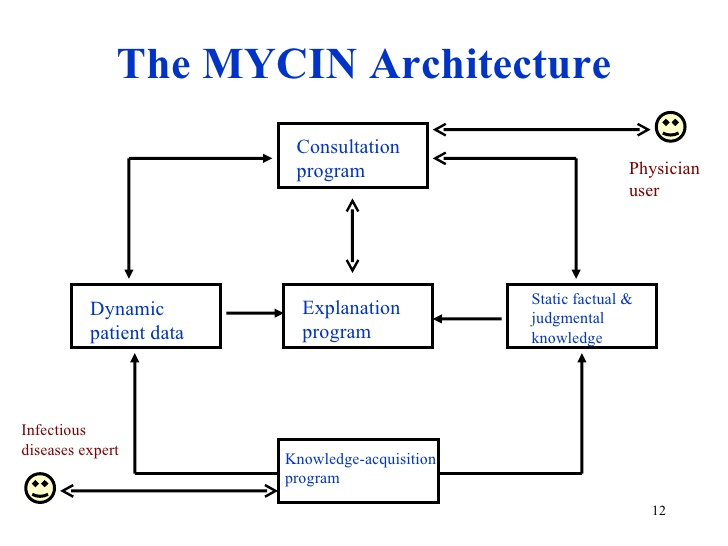
\includegraphics[width=100mm, height = 80mm]{images/mycin.jpg}
\caption{MYCIN Architecture(Source: slideshare.net)}
\end{center}
\end{figure}
\subsection{Chronic Kidney Disease Prediction Using Back Propagation Neural Network Algorithm}
This system of neural network accepts disease-symptoms as input and it is trained according to various training algorithms. Levenberg, Bayesian regularization, Scaled Conjugate and Resilient back propagation algorithm are discussed here. After neural network is trained using back propagation algorithms, this trained neural network system is used for detection of kidney disease in the human body. The back propagation algorithms presented here have capacity for distinguishing amongst infected patients or non-infected person.
\section{Automated Disease Prediction System (ADPS): A User Input-based Reliable Architecture for Disease Prediction}
Automated  Disease  Prediction System  (ADPS)  that  relies  on guided  (to be  described later)  user input.  The system  takes input from the user and provides a list (topmost diseases have greater  likelihood  of occurrence)  of  probable  diseases.  The accuracy of ADPS has been evaluated extensively. It ensured an average of 14.35\% higher accuracy in comparison with the existing solution. \par
In  this  paper,  the  contribution  includes  proposing  a  new disease prediction framework (ADPS) that takes into account symptom  names  as  well  as  other  vital  parameters to improve disease prediction accuracy and  proposing  techniques  to allow  greater  linguistic  diversity  so  that  users  do  not  feel uncomfortable while giving input. \par
It is presumed that the user will give text input in one sentence describing  a  single  symptom  at  a  time  (guideline  for  user input). Subsequent symptoms can be added in new lines. After getting user input, the system will scan through each line and tag  each  word  according  to  their relevant  parameter.  Then after performing certain computations (to be described later) the  system  will  return  a  list  of  possible  diseases  ordered according to the likelihood of their occurrences.

\section{Neural Network Based Intelligent System for Predicting Heart Disease}

This paper proposed an intelligent automated system incorporating  the  techniques of data mining with machine learning in order to make decisions. Medical practitioners are being assisted by  the  automated  systems  for  providing effective  treatment  [18].  Data  mining  techniques  involves  a combination  of  statistical  methods  with  machine  learning algorithms  .Data  mining  techniques  help  the  system  in analyzing the symptoms and machine learning methodshelp in  predicting  the  disease  based  on  the  analysis  performed [13,20].  The  advantage  of  this  automated  system  is  that  it predicts the  disease  in  a  less  amount  of  time as  well  in less cost.  Therefore,  more  research  is  carried  out  in  the  field  of machine   intelligence   to   improvise   the   system   for   an effective   prediction.   This   paper   proposed   an   intelligent system    developed    using    the    concept    of    Multilayer Perceptron Neural Network with Back Propagation Algorithm,  as a practitioner  needs  to  make  a  decision  from multiple inputs such as current and previous medical history of  a  patient.  \par Neural  networks  are  proved  to  be  effective  in making decisions by predicting the data. As the inputs used in  predicting  the  disease  are  more  in  number  and  diagnosis has to be performed at different stages, Multilayer Perceptron  based  neural networks  are  used  in this  proposed system.  Neural  Network  extends  its  predictive  capability  at different  hierarchical  levels  in  a  multi-layered  structure  of networks.  This  multi-layered  structure helps  in  selecting features from the dataset at different scales in order to refine them  into  more  specific  features.  To  facilitate  this,  the concept of Multi-layer Perceptron Neural Network has been introduced through the implementation of Back-propagation algorithm  for  efficient  diagnosis  of  heart  disease.  In  this paper, 14 attributes are used as inputs for training the system of  neural  networks  for  diagnosing  heart  disease  risk  level using multi-layered network.Traditional   diagnosing   approaches   have   no proper automated   tools   use   for   the   purpose   of   heart   disease diagnostic   system.   The   commonly   used   data   mining algorithms for predicting diseases are: Genetic algorithm, K-means algorithm, MAFIA algorithm. Several methods proposed the implementation of classification  algorithms  in  diagnosis  of  heart  disease  and resulted with an accuracy of 88.33%





 
\chapter{Methodology}

\section{System Process Model}
\subsection{Incremental Software Development Model}
Incremental Model is a process of software development where requirements are broken down into multiple standalone modules of software development cycle. Incremental development is done in steps from analysis design, implementation, testing/verification, maintenance.\par
Each iteration passes through the requirements, design, coding and testing phases. And each subsequent release of the system adds function to the previous release until all designed functionality has been implemented.\par
The system is put into production when the first increment is delivered. The first increment is often a core product where the basic requirements are addressed, and supplementary features are added in the next increments. Once the core product is analyzed by the client, there is plan development for the next increment.
	
	
	
\begin{figure}[h]
\begin{center}
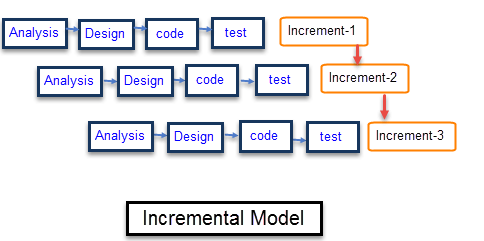
\includegraphics[width=100mm, height = 70mm]{images/Incremental.png}
\caption{Incremental Development Model(Source: researchgate.net)}
\end{center}
\end{figure}
\pagebreak

\begin{itemize}

\item 1st incremental: We have done research regarding our project idea and list out the functional and non-functional requirements of our project. We start writing our documentation. We study the feasibility of our project in term of economical, technical and operational.

\item 2nd incremental: Familarizing with tools like jupyter notebook, android studio and flask framework. We made a prototype of our project and consulted with our supervisor. We research and collected dataset which were appropriate for our project. We prepared those collected data for use in our machine learning training. We trained our dataset using various classification algorithms like Random Forest, Decision Tree and Back Propagation and compare the performance of different algorithms using confusion matrix. From above analysis we conclude that Back Propagation was optimal for our project.

\item 3rd incremental: Tuning the performance of back propagation model to get optimal result. We analysis our model to get optimal value of hyper parameters like number of hidden layers, learning rate, activation function, Epoch.

\item 4th incremental: After obtaining optimal neural network model of our project we deployed our model in server running on flask frame work. We create RESTful API and create user interface for android devices.

\end{itemize}




\section{Reason of using  Python ?}
We found out that python was great choice machine learning implementation in our project because of two simple reasons
\begin{itemize}
\item Simplicity: When it comes to big data or just very complex decision-making path, the simplicity is the key. Python is well-known for its readability, developer-friendly syntax, and semantics. The less the developer has to worry about the code itself, the more focus and emphasis can be put on finding solutions. Moreover, the Python community is huge and constantly growing, which is also a plus point for a language.
\item Libraries and frameworks : What makes Python so suitable is the amount of ready, open source libraries and frameworks. In our project for many data related tasks like importing dataset, formatting dataset, data visualization, statistics about dataset we are using numpy, pandas library. Using these library saves a lot of time and energy.

\end{itemize}



\section{Why this project?}
As Nepal is a developing country. Health Cares, doctors, hospitals have not reached at every corner of the country specially on the rural areas. So, we came with the idea of doing this project that uses AI to provide health care facilities through our mobile application.\par  
Artificial intelligence in healthcare is the use of complex algorithms and softwares to estimate human cognition in the analysis of complicated medical data. The primary aim of health-related AI applications is to analyze relationships between prevention or treatment techniques and patient outcomes.\par
AI technology from traditional technologies in health care is the ability to gain information, process it and give a well-defined output to the end-user. AI does this through machine learning algorithms. These algorithms can recognize patterns in behavior and create its own logic. In order to reduce the margin of error, AI algorithms need to be tested repeatedly. AI algorithms behave differently from humans in two ways: 
\begin{itemize}
    \item Algorithms are literal: If you set a goal, the algorithm can't adjust itself and only understand what is has been told explicitly
    \item Algorithms are black boxes: Algorithms can predict extremely precise, but not the cause or the why.
\end{itemize}
The primary aim of health-related AI applications is to analyze relationships between prevention or treatment techniques and patient outcomes.[2] AI programs have been developed and applied to practices such as diagnosis processes, treatment protocol development, drug development, personalized medicine, and patient monitoring and care.\par
Hence, AI is reshaping the health care industry by helping to predict and scan diseases, detect injuries, and help people maintain good health even on a day-to-day basis with easy-to-use mobile applications.

WeCare-Your Personal Heath Assistance is a AI based project focused on making sure that patients take the right medications at the right time. For that purpose, we use technologies like user friendly interface, preventive measures and overview of the disease, pill reminder which can help people to predict the disease with the ongoing symptoms that they are suffering and help them to maintain good health.

\section{App Development Process}
There are currently over 38.3 million smart phone user in Nepal which is 34\% higher than the population of Nepal. As the number of internet users in Nepal has increased rapidly, actually 63 percent of the total population currently connect to the internet. So, android apps are no longer just a need; it has become a part of the business strategy.\par
Android app development is significant as Android owns over seventy-five percent market share globally. And this number is expected to grow more. Business houses have started realizing the true potential of Android apps. The latest version, Android Q, has come with the more security and simplifying features for the users and businesses. Websites lack mobile apps in user experience, and nowadays, every business has an online presence. So, to stay ahead of others, Android app development is crucial.\par

Every app requirement that we come across has different requirements and different functionality. 
However, the Android app development process is a sum-mean of all stages that go into designing, creating, developing and post-deployment of the app.

Android app development process step:

\begin{itemize}

\item Conceptualization: It is the most significant stage in the development process of Android application as we refine the app idea into a solid base of the application. \par
During this stage, we evaluated all the necessary work for the following process. It is also beneficial to research and brainstorming before jumping to the next step. 

\item Feasibility Assessment: User can clearly understands the app visuals through detailed sketches of the conceptualized product to refine their ideas and arrange design components in a precise manner.\par
By the end of feasibility testing, we had the idea of our app whether it is functionaly feasible or not. 

\item Design: In this phase of the Android development, we design our app's UI user interaction interface by keeping in mind the modern user’s preference. The user interface for an Android app is built using a hierarchy of layouts and widgets.Layouts are containers that control how their child views are positioned on the screen. Widgets are UI components such as buttons and text boxes.Most of our UI is defined in XML files using Android Studio's Layout Editor, which makes it easy to build a layout by drag-and-dropping views.\par 
As application designing is a multi-step process so we used this phase for drawing clear visual directions of the final app development.

\item Development: During this stage, we developed a working prototype to validate the functionality, assumptions, and understanding of the project scope. The app goes through a set of steps as the development progresses from core functionality development to light testing.

\item Testing and Debugging: It is one of the critical components of any app development process, it is always a great idea to test at early stages. \par
We tested our app for usability, interface & security checks, stress, compatibility, and performance to find bugs or errors in app and if found then can be fixed in testing phase. 
\end{itemize}




\section{Procedure for Medical Diagnosis}
\subsection{Data Collection}
This is most essential step in machine learning project. Predictive models are only as good as the data from which they are built, so good data collection practices are crucial to developing high-performing models. To train our model, we need dataset that contain information about diseases and its respective symptoms.\newline
Here is some information about the dataset which we obtained from UCI machine learning repository.
\begin{itemize}
    \item Total Number of unique Diseases: 34
    \item Total Number of symptoms: 132
    \item Total Number of entities in dataset: 4920
     
\end{itemize}

\begin{figure}[h]
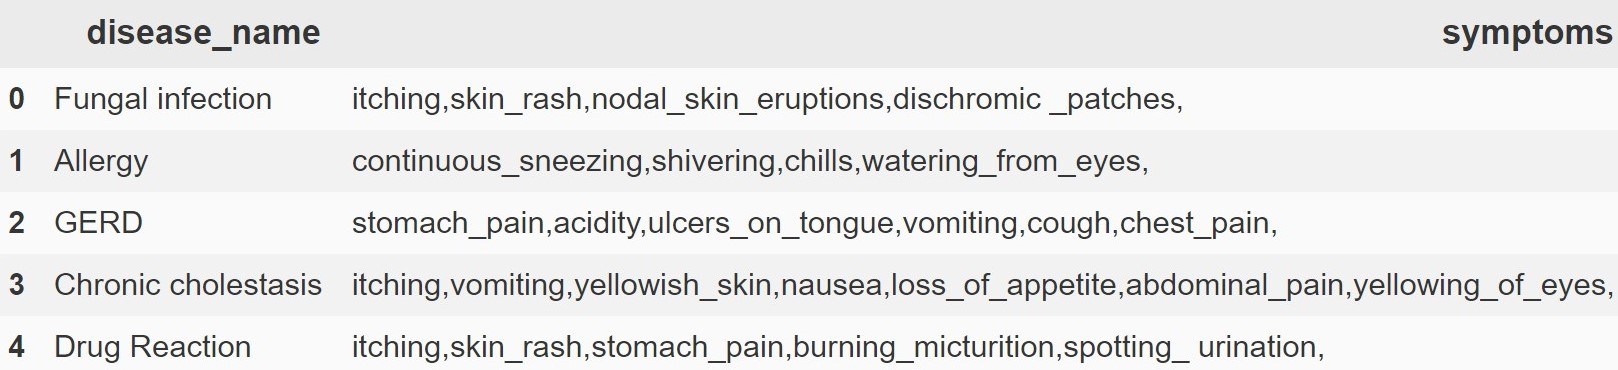
\includegraphics[width=160mm,height=40mm]{dataset_summary/diseaseAndSymptoms.jpg}
 \caption{Sample of dataset}
\end{figure}

\begin{figure}[H]
 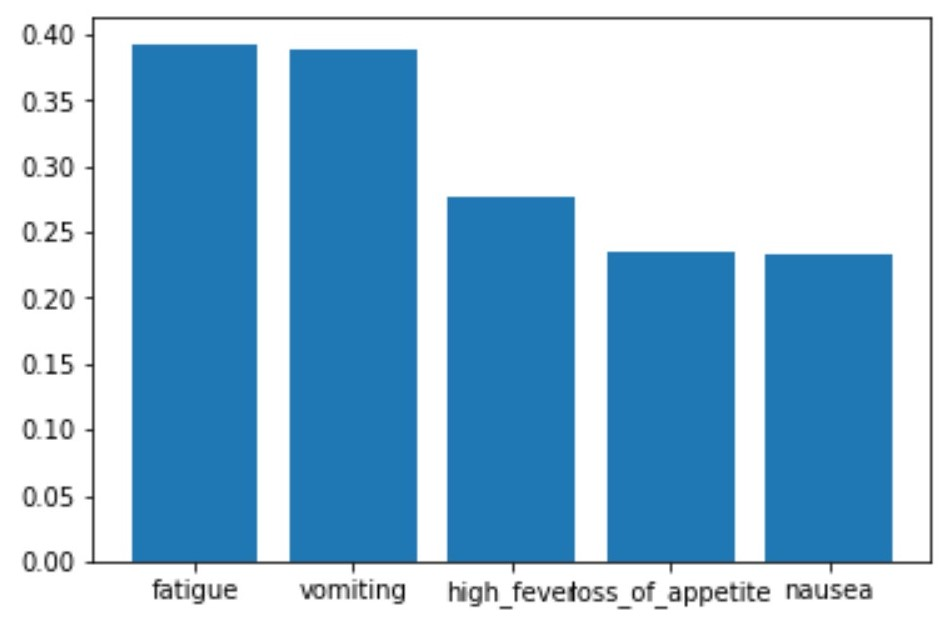
\includegraphics[width=150mm,height=70mm]{dataset_summary/top5Disease.jpg}
 \caption{Top five most common symptoms}
\end{figure}

\subsection{Data Preparation}
Most machine learning algorithms require data to be formatted in a very specific way, so datasets generally require some amount of preparation before they can yield useful insights. Some datasets have values that are missing, invalid, or otherwise difficult for an algorithm to process. If data is missing, the algorithm can’t use it. If data is invalid, it causes the algorithm to produce less accurate or even misleading outcomes. Good data preparation produces clean and well-curated data that leads to more practical, accurate model outcomes. \\ Also to train the model we need to split the dataset in train dataset & test dataset, the test dataset will be used for model evaluation.

\subsection{Choosing a Machine Learning Algorithms}
When we look at machine learning algorithms, there is no one solution or one approach that fits for all king of problems. There are several factors such as 
     \begin{itemize}
         \item {Type of problem}  
         \item {Size of training set}
         \item {Accuracy}
         \item  {Number of features}
     \end{itemize}

That can affect your decision to choose a machine learning algorithm. Since our project associated with the supervised learning problem, there are different supervised learning algorithms like KNN, Random Forest, Decision Tree, ANN etc.



\section{Introduction to Biological neural network}
A neural network consists of numbers of non-linear computational elements called neurons or node. These neurons are connected to each other. The concept of neural network developed from way a human behaves. The way neurons work in the human brain is tried to be used in neural network. A neuron's dendrite tree is connected to thousand neighbour neurons. When one neurons fire a positive or negative charge it is received by the dendrites. The strength of all the charges fired is added together through the process of spatial and temporal summation. Spatial summation occurs when several weak signals are converted into a single large one, while the temporal summation converts a rapid series of weak pulses from one source into a large signal. \newline
The dendrites serve as receptors for signals from other neurons, whereas the purpose of an axon is transmission of the generated neural activity to other neurons. The aggregate inputs are then passed to the soma(cell body). If the aggregate is greater then the axon hillock's threshold value, then the neuron fires and an output signal is transmitted down to axon. The strength of the output is constant regardless of whether the input was just above the threshold, or hundred times greater. The output strength is unaffected by the many divisions in the axon; it reaches each terminal button with the same intensity it had at the axon hillock. \newline
Each terminal button is connected to other neurons across a small gap called synapse. The physical and neuro-chemical characteristics of each synapse determine the strength and the polarity of the new input signal. This process repeats itself across all neurons.

 \begin{figure}[h]
   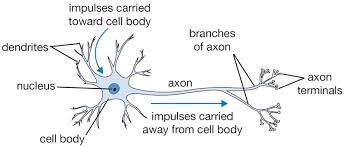
\includegraphics[width=130mm,height=80mm]{images/bio.jpg}
   \caption{Biological Neural Network}
        
   \end{figure}

  \textbf{Characteristics of Biological Neural Network} \newline
Some of the characteristics of the biological neural network that make it superior to the most sophisticated AI computer system for the pattern tasks are the following:
\begin{itemize}
    \item Robustness and fault tolerance: The decay of the nerve cell does not seem to affect the performance significantly.
    \item Flexibility: The network automatically adjusts to a new environment without any preprogrammed instruction.
    \item Ability to deal with various types of data situation: The network can deal with situations that are fuzzy, probablistic, noisy and inconsistence.
    \item Collective computation: The network performes routinely many operations in parallel and also a given task in a distributed manner.
     
\end{itemize}


\section{Artificial Neural Network}
ANN is a mathematical structure composed of highly interconnected elements that are capable of modeling complex nonlinear relationship. A feed-forward multilayer per-ceptron network which usually adapts error back propagation in training state is the most popular ANN paradigm that is performs well in nonlinear problems. There are two types of ANN namely,  supervised ANN and unsupervised ANN. Unsupervised ANN doesn’t require output for guiding the weight adjustment whereas for supervised ANN the model is trained based on comparison of the output and target until the model output matches the target.

   \begin{figure}[h]
   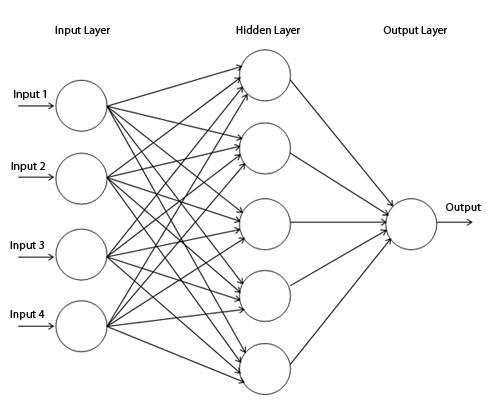
\includegraphics[width=120mm,height=70mm]{neuralNetwork/neuralNetwork.jpg}
   \caption{Neural Network (Source: researchgate.net)}
        
   \end{figure}
\subsection{Elements of a Neural Network }
 
  \begin{itemize}
      \item \textbf{Input Layer}: This layer accepts input features. It provides information from the outside world to the network, no computation is performed at this layer, nodes here just pass on the information(features) to the hidden layer.
      \item \textbf{Hidden Layer}: Nodes of this layer are not exposed to the outer world, they are the part of the abstraction provided by any neural network. Hidden layer performs all sort of computation on the features entered through the input layer and transfer the result to the output layer.
      \item \textbf{Output Layer}: This layer bring up the information learned by the network to the outer world.
      \item  \textbf{Neuron}: The basic unit of computation in a neural network is the neuron, often called a node or unit. It receives input from some other nodes, or from an external source and computes an output.
      \item \textbf{Bias}: Bias is an additional parameter in the Neural Network which is used to adjust the output along with the weighted sum of the inputs to the neuron. Therefore Bias is a constant which helps the model in a way that it can fit best for the given data.
      \item \textbf{Activation Function}: Activation function decides, whether a neuron should be activated or not by calculating weighted sum and further adding bias with it. The purpose of the activation function is to introduce non-linearity into the output of a neuron. A neural network without an activation function is essentially just a linear regression model. The activation function does the non-linear transformation to the input making it capable to learn and perform more complex tasks. \par
         Every activation function (or non-linearity) takes a single number and performs a certain fixed mathematical operation on it. There are several activation functions you may encounter in practice like sigmoid, reLU, tanh.
      \item \textbf{Learning rate}: learning rate is a hyperparameter that controls how much to change the model in response to the estimated error each time the model weights are updated. Choosing the learning rate is challenging as a value too small may result in a long training process that could get stuck, whereas a value too large may result in learning a sub-optimal set of weights too fast or an unstable training process.
   
      \end{itemize}
      
 \section{Biological vs Artificial Neural Network}
An artificial neural network is basically a mathematical model built from simple functions with changing parameters. Just like a biological neuron has dendrites to receive signals, a cell body to process them, and an axon to send signals out to other neurons, the artificial neuron has a number of input channels, a processing stage, and one output that can fan out to multiple other artificial neurons. Although artificial neurons and perceptrons were inspired by the biological processes scientists were able to observe in the brain back in the 50s, they are vastly different in terms of both their structure and workings.

\textbf{Size:} Our brain contains about 86 billion neurons and more than a 100 trillion synapses. The number of “neurons” in artificial networks is much less than that but comparing their numbers this way is misleading. Perceptrons just take inputs on their “dendrites” and generate output on their “axon branches”. A single layer perceptron network consists of several perceptrons that are not interconnected: they all just perform this very same task at once. Deep Neural Networks usually consist of input neurons, output neurons and neurons in the hidden layers, in-between. All the layers are usually fully connected to the next layer. Manual feature extraction requires human brain power which is also not taken into account when summing up the number of “neurons” required for Deep Learning tasks. The limitation in size isn’t just computational: simply increasing the number of layers and artificial neurons does not always yield better results in machine learning tasks.

\textbf{Topology:} All artificial layers compute one by one, instead of being part of a network that has nodes computing asynchronously. Feedforward networks compute the state of one layer of artificial neurons and their weights, then use the results to compute the following layer the same way. During backpropagation, the algorithm computes some change in the weights the opposing way, to reduce the difference of the feedforward computational results in the output layer from the expected values of the output layer. In biological networks, neurons can fire asynchronously in parallel, have small-world nature with a small portion of highly connected neurons and a large amount of lesser connected ones. Since artificial neuron layers are usually fully connected, this small-world nature of biological neurons can only be simulated by introducing weights that are 0 to mimic the lack of connections between two neurons.

\textbf{Speed:} Certain biological neurons can fire around 200 times a second on average. Signals travel at different speeds depending on the type of the nerve impulse. Action potential frequency carries information for biological neuron networks: information is carried by the firing frequency or the firing mode (tonic or burst-firing) of the output neuron and by the amplitude of the incoming signal in the input neuron in biological systems. Information in artificial neurons is instead carried over by the continuous, floating point number values of synaptic weights. How quickly feedforward or backpropagation algorithms are calculated carries no information, other than making the execution and training of the model faster. They are functions that can be calculated as many times and as fast as the computer architecture would allow. 

\textbf{Fault-tolerance:} Biological neuron networks due to their topology are also fault-tolerant. Information is stored redundantly so minor failures will not result in memory loss. They don’t have one “central” part. The brain can also recover and heal to an extent. Artificial neural networks are not modeled for fault tolerance or self regeneration,though recovery is possible by saving the current state (weight values) of the model and continuing the training from that save state. Dropouts can turn on and off random neurons in a layer during training, mimicking unavailable paths for signals and forcing some redundancy. Trained models can be exported and used on different devices that support the framework, meaning that the same artificial neural network model will yield the same outputs for the same input data on every device it runs on. Training artificial neural networks for longer periods of time will not affect the efficiency of the artificial neurons.  Another difference is, that all processes (states and values) can be closely monitored inside an artificial neural network.

\textbf{Power consumption:} The brain consumes about 20\% of all the human body’s energy-despite it’s large cut, an adult brain operates on about 20 watts (barely enough to dimly light a bulb) being extremely efficient. For benchmark: a single Nvidia GeForce Titan X GPU runs on 250 watts alone, and requires a power supply instead of beef tallow. Our machines are way less efficient than biological systems. Computers also generate a lot of heat when used, with consumer GPUs operating safely between 50–80 degrees Celsius instead of 36.5–37.5 °C.
 Biological neural networks use very little power compared to artificial networks.

\textbf{Signal transport and processing:} An action potential is either triggered or not — biological synapses either carry a signal or they don’t. Perceptrons work somewhat similarly, by accepting binary inputs, applying weights to them and generating binary outputs depending on whether the sum of these weighted inputs have reached a certain threshold. Artificial neurons accept continuous values as inputs and apply a simple non-linear, easily differentiable function (an activation function) on the sum of its weighted inputs to restrict the outputs’ range of values. The human brain works asynchronously, ANNs work synchronously.

\textbf{Learning:} We still do not understand how brains learn, or how redundant connections store and recall information. By learning, we are building on information that is already stored in the brain. Artificial neural networks in the other hand, have a predefined model, where no further neurons or connections can be added or removed. Only the weights of the connections can change during training. The networks start with random weight values and will slowly try to reach a point where further changes in the weights would no longer improve performance. Learning can be understood as the process of finding optimal weights to minimize the differences between the network’s expected and generated output: changing weights one way would increase this error, changing them the other way would decrees it. The rate of how artificial neural networks learn can change over time.\par
Training (backpropagation using an optimization method like stochastic gradient descent, over many layers and examples) is extremely expensive, but using a trained network (simply doing feedforward calculation) is ridiculously cheap. Unlike the brain, artificial neural networks don’t learn by recalling information — they only learn during training, but will always “recall” the same, learned answers afterwards, without making a mistake. These are all considerable differences between biological and artificial neurons.


 
\section{Back Propagation Neural Network Algorithm}
Back Propagation, an abbreviation for “backward propagation of errors”, is a common method of training artificial neural networks. From a desired output, the network leans from many inputs, similar to the way a child learns to identify a dog from examples of dogs. Back propagation is a neural network learning algorithm. The feedback forward network structure is most important ANN structure. Design of a feed forward net for any specific application involves many issues, most of which require problem dependent solutions. The overall computational approach comprising of two parts: feed forward implementation of learned mapping and training of 3 layer network.\par
Back Propagation Neural is a multilayer neural network consisting of the input layer, at least one hidden layer and output layer. As its name suggests, back propagating will take place in this network. The error which is calculated at the output layer, by comparing the target output and the actual output, will be propagated back towards the input layer.
 

\subsection{Architecture of Back propagation}
As shown in the diagram, the architecture of Back Propagation Network has three interconnected layers having weights on them. The hidden layer as well as the output layer also has bias, whose weight is always 1, on them. As is clear from the diagram, the working of Back Propagation Network is in two phases. One phase sends the signal from the input layer to the output layer, and the other phase back propagates the error from the output layer to the input layer.

  \begin{figure}[h]
  \begin{center}
  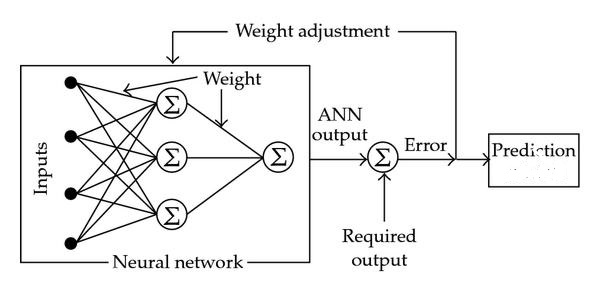
\includegraphics[width=120mm,height=80mm]{images/ANNBack.jpg}
  \caption{ANN architecture with back-propagation algorithm.(Source: researchgate.com)}
  \end{center}
  \end{figure}  
   
  \pagebreak
  \subsection{A Pseudo-Code Algorithm} 
\begin{itemize}
\item Randomly choose the initial weights
\item While error is too large \par
-For each training pattern (presented in random order)
\begin{itemize}
   
 \item Apply the inputs to the network
    \item Calculate the output for every neuron from the input layer, through the hidden layer(s), to the output layer
    \item Calculate the error at the outputs
    \item Use the output error to compute error signals for pre-output layers
    \item Use the error signals to compute weight adjustments
    \item Apply the weight adjustments \par

\end{itemize}
-Periodically evaluate the network performance 
\end{itemize}  
\subsection{Training/learning  Model}  
The training process of the MLP occurs by continuous adjustment of the weights of the connections after each processing. This adjustment is based on the error in output(which is the different between the expected result and the output). This continuous adjustment of the weights is a supervised learning process called ‘backpropagation’.\newline
The backpropagation algorithm consists of two parts:
\newline
1.forward pass\newline
2.backward pass\newline
In the forward pass, the expect output corresponding to the given inputs are evaluated.
In the backward pass, partial derivatives of the cost function with respects to the different parameters are propagated back through the network.\newline
The process continues until the error is at the lowest value.
\pagebreak
\subsection{Basic Neuron Model In A Feedforward Network}
\begin{itemize}
    \item Inputs x\textsubscript{i} arrive through pre-synaptic connections 
    \item Synaptic efficacy is modeled using real weights w\textsubscript{i}
    \item The response of the neuron is a nonlinear function f of its weighted inputs
\end{itemize}

 \begin{figure}[h]
  \begin{center}
  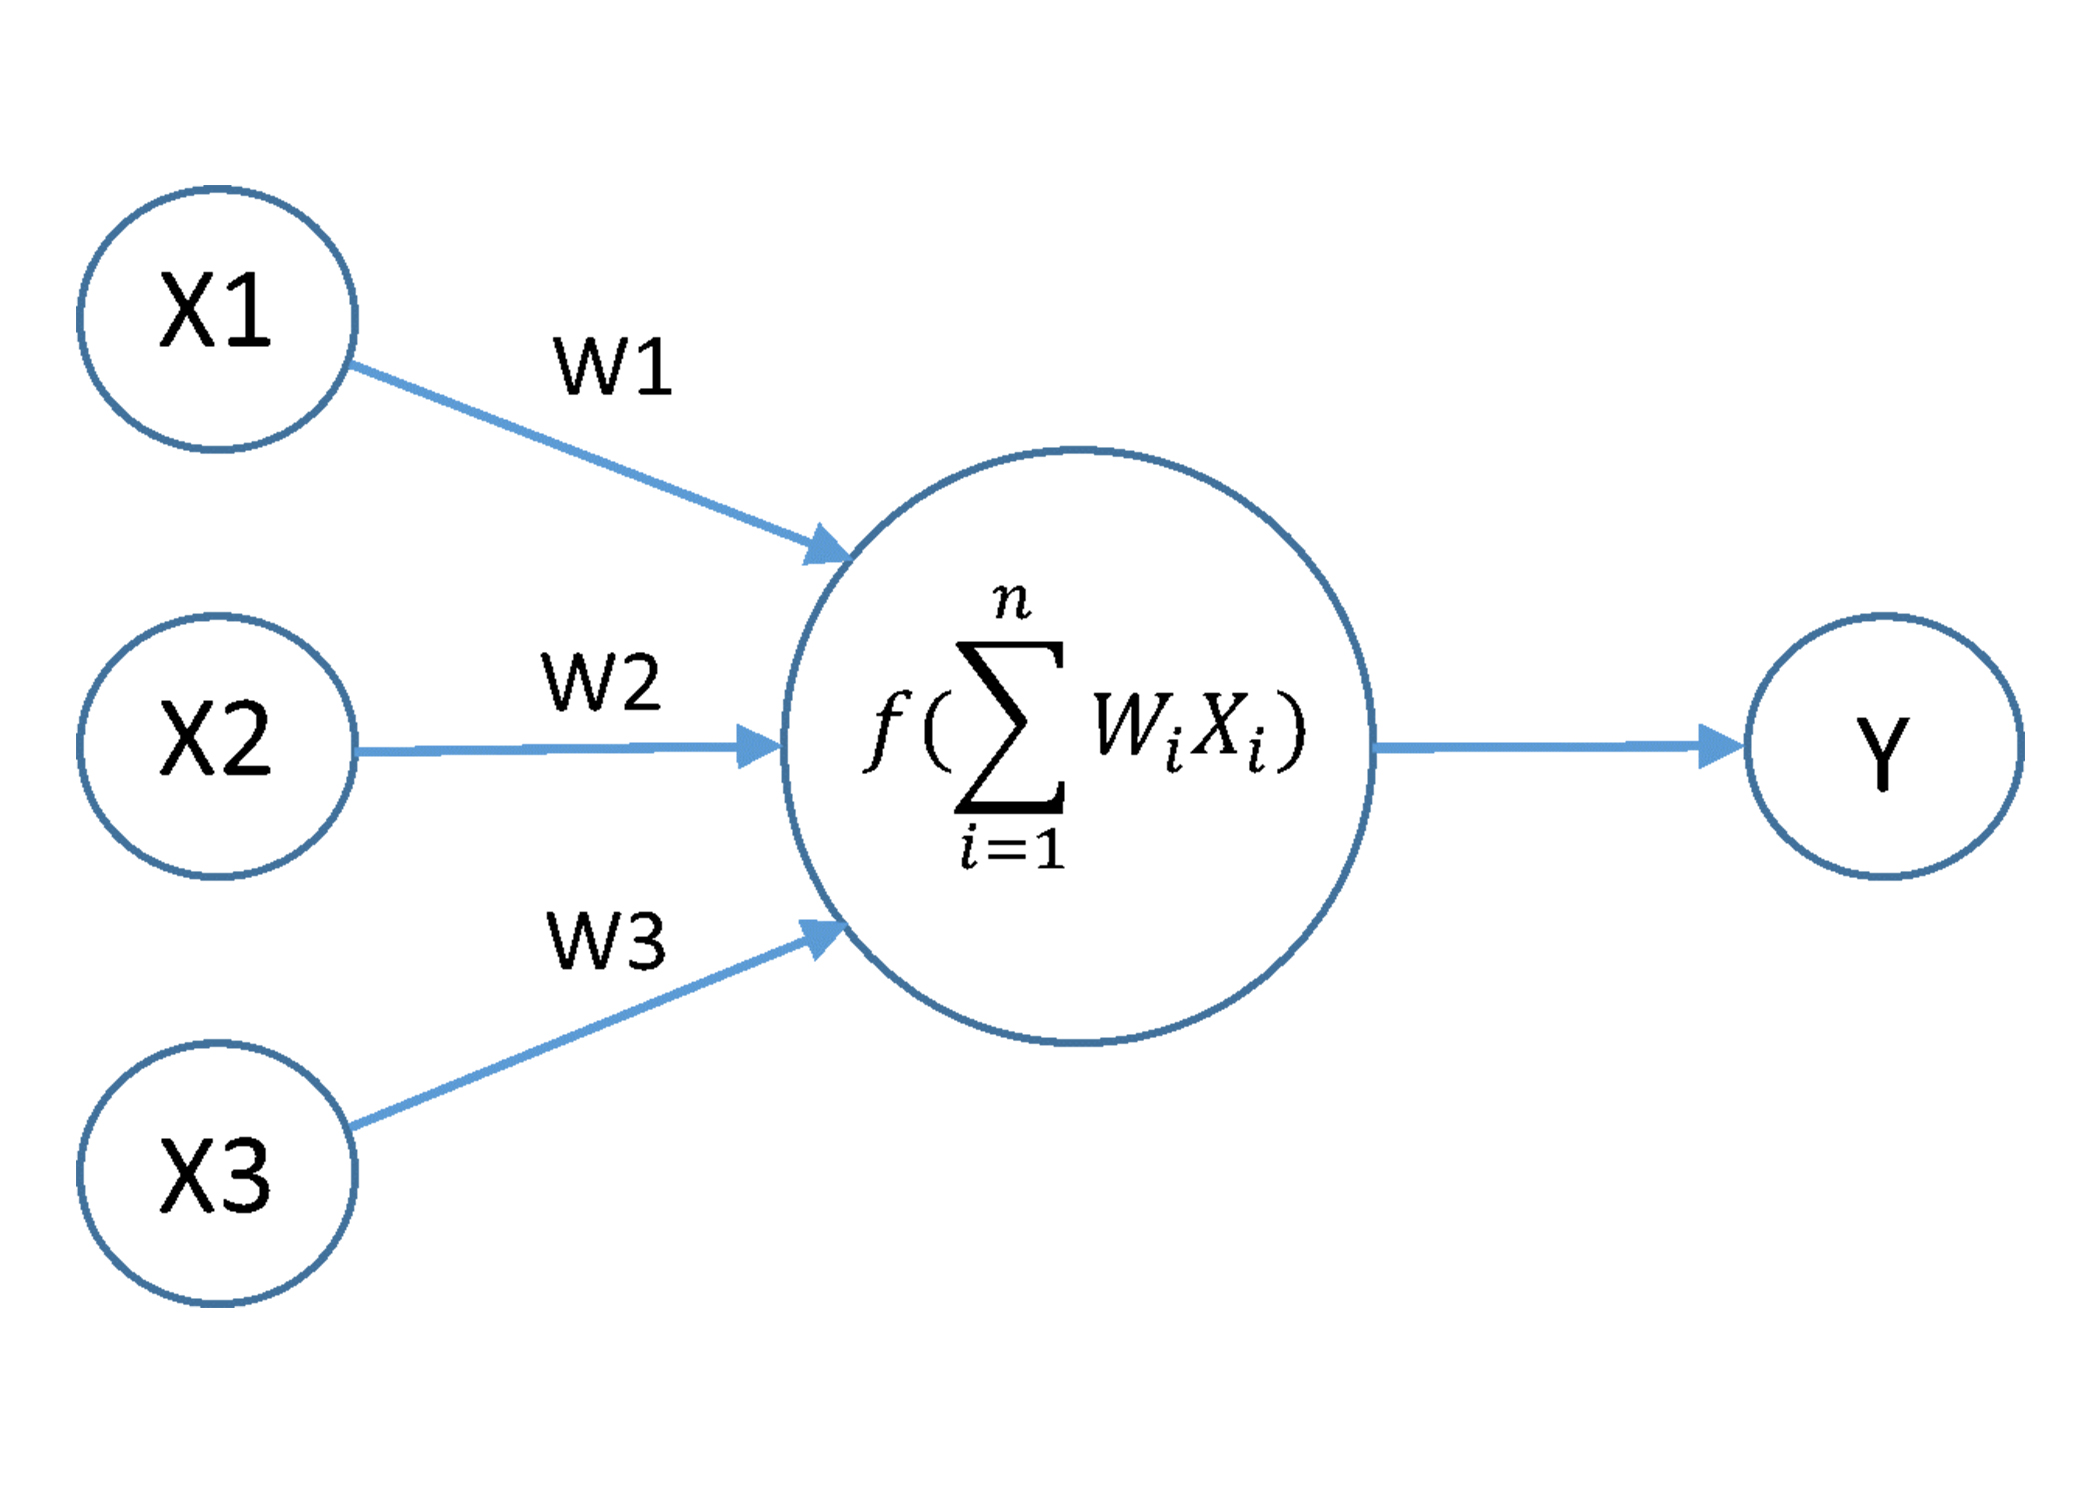
\includegraphics[width=100mm,height=70mm]{images/feedforward.jpg}
  \caption{Neuron Model Feedforward Network(Source: edureka.co)}
  \end{center}
  \end{figure}   
  
\subsection{Inputs To Neurons}
\begin{itemize}
    \item Arise from other neurons or from outside the network
    \item Nodes whose inputs arise outside the network are called input nodes and simply copy values
    \item An input may excite or inhibit the response of the neuron to which it is applied, depending upon the weight of the connection
\end{itemize}

\subsection{Weights}
\begin{itemize}
    \item Represent synaptic efficacy and may be excitatory or inhibitory
    \item Normally, positive weights are considered as excitatory while negative weights are thought of as inhibitory
    \item Learning is the process of modifying the weights in order to produce a network that performs some function
\end{itemize}

\subsection{Outputs}
\begin{itemize}
    \item The response function is normally nonlinear
    \item Samples include \par
    
        $$f(x) &= 1/1+exp^{-\sigma x}$$
    

\end{itemize}  

\subsection{Network Error}
\begin{itemize}
    \item Total-Sum-Squared-Error (TSSE)
    
       $$TSSE &=  \sum_{patterns}\sum_{outputs} (desire-actual)^2$$
    
    \item Root-Mean-Squared-Error (RMSE)
    
$$RMSE &= \sqrt{\frac{2*TSSE}{&#patterns * &#outputs }}$$
        
 \end{itemize}




\subsection{Calculate Outputs For Each Neuron Based On The Pattern}
\begin{itemize}
    \item The output from neuron j for pattern p is O\textsubscript{pj} where

    $$O\textsubscript{pj}(net\textsubscript{j}) &= 1/1+exp^{-\sigma netj}$$
    
    and 
    $$ (net\textsubscript{j}) &= bias*W\textsubscript{bias} &+ \sum_{k} O\textsubscript{pk} W\textsubscript{kj}$$
    where k ranges over the input indices and W\textsubscript{jk} is the weight on the connection from input k to neuron j
\end{itemize}

 \begin{figure}[h]
  \begin{center}
  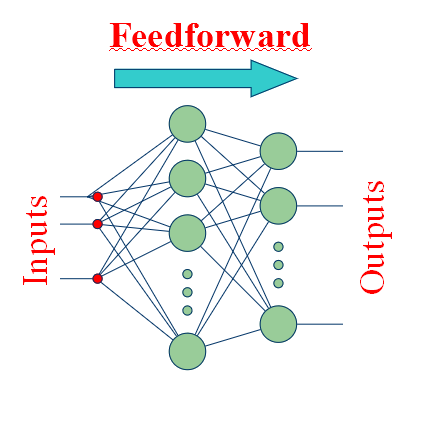
\includegraphics[width=120mm,height=80mm]{images/feed.PNG}
  \caption{Feedforward Network Model(Source: edureka.co)}
  \end{center}
  \end{figure}   
  
\subsection{Calculate The Error Signal For Each Output Neuron}
\begin{itemize}
    \item The output neuron error signal $\Delta$ pj is given by 
    $$ \Delta pj &= (T\textsubscript{pj} &- O\textsubscript{pj}) O\textsubscript{pj} (1 &- O\textsubscript{pj})$$
    \item T\textsubscript{pj} is the target value of output neuron j for pattern p
    \item O\textsubscript{pj} is the actual output value of output neuron j for pattern p
    
\end{itemize}  

\subsection{Calculate The Error Signal For Each Hidden Neuron}
\begin{itemize}
    \item The hidden neuron error signal $\partial$ pj is given by
        $$\partial pj &=  O\textsubscript{pj} (1 &- O\textsubscript{pj}) \sum_{k} \partial \textsubscript{pk}  W\textsubscript{jk}$$

	where $\partial$ pk is the error signal of a post-synaptic neuron k and W\textsubscript{jk} is the weight of the connection from hidden neuron j to the post-synaptic neuron k 
    
\end{itemize}  

\subsection{Calculate And Apply Weight Adjustments}
\begin{itemize}
    \item weight adjustments $\delta$ W\textsubscript{ji} at time t by\\*
     $\Delta$ W\textsubscript{ji}(t) &= η \partialj O\textsubscript{pi}

    \item Apply weight adjustments according to\\*
W\textsubscript{ji}(t+1) = W\textsubscript{ji}(t) + $\Delta$ W\textsubscript{ji}(t)

    \item Some add a momentum term \\* $\alpha$ &* $\Delta$Wji(t-1)
    
\end{itemize}



  
  \subsection{Summarization of Steps}
\begin{itemize}
\item Calculate the error – How far is your model output from the actual output.
\item Minimum Error – Check whether the error is minimized or not.
\item Update the parameters – If the error is huge then, update the parameters (weights and biases). After that again check the error. Repeat the process until the error becomes minimum.
\item  Model is ready to make a prediction – Once the error becomes minimum, you can feed some inputs to your model and it will produce the output.
  \end{itemize}
  

 
\section{System Analysis}
\subsection{System Flow Diagram}
\begin{figure}[H]
\begin{center}
    
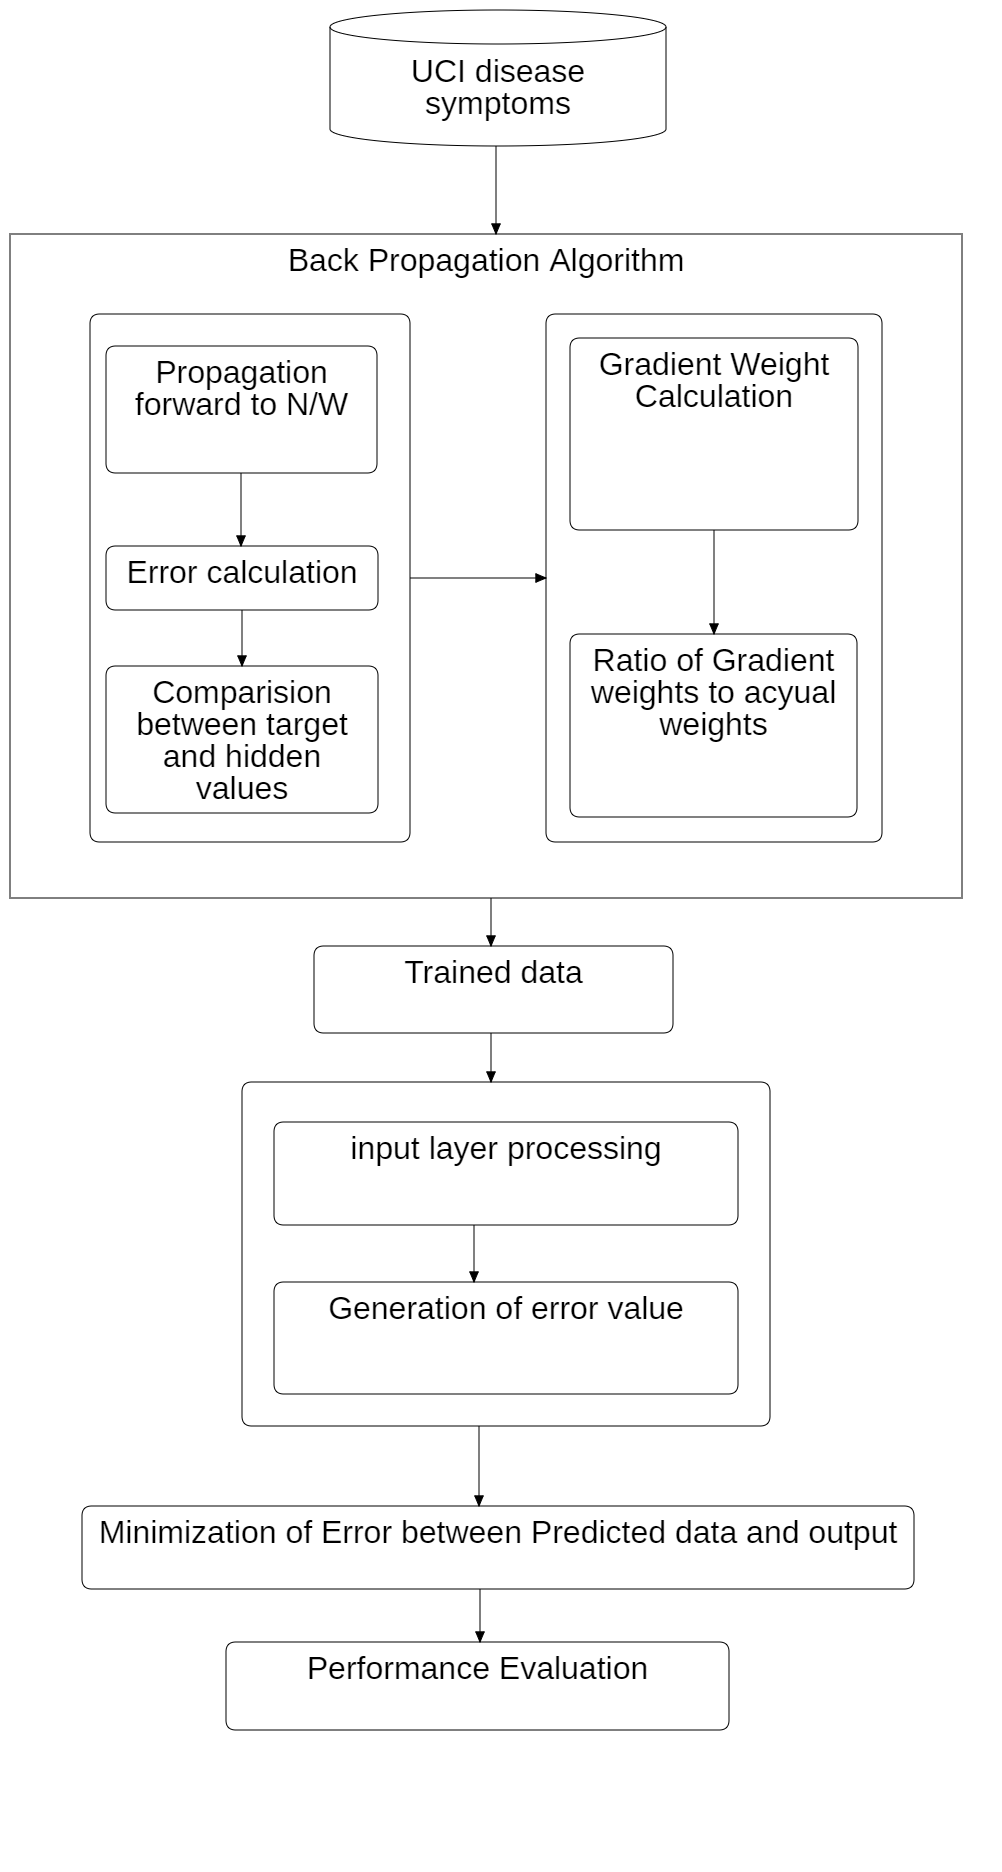
\includegraphics[width=140mm,height=205mm]{images/flow.png}
 \caption{System Flow Diagram of Proposed system}
 \end{center}                
\end{figure}

\subsection{Usecase Diagram}
\begin{figure}[H]
\begin{center}
    
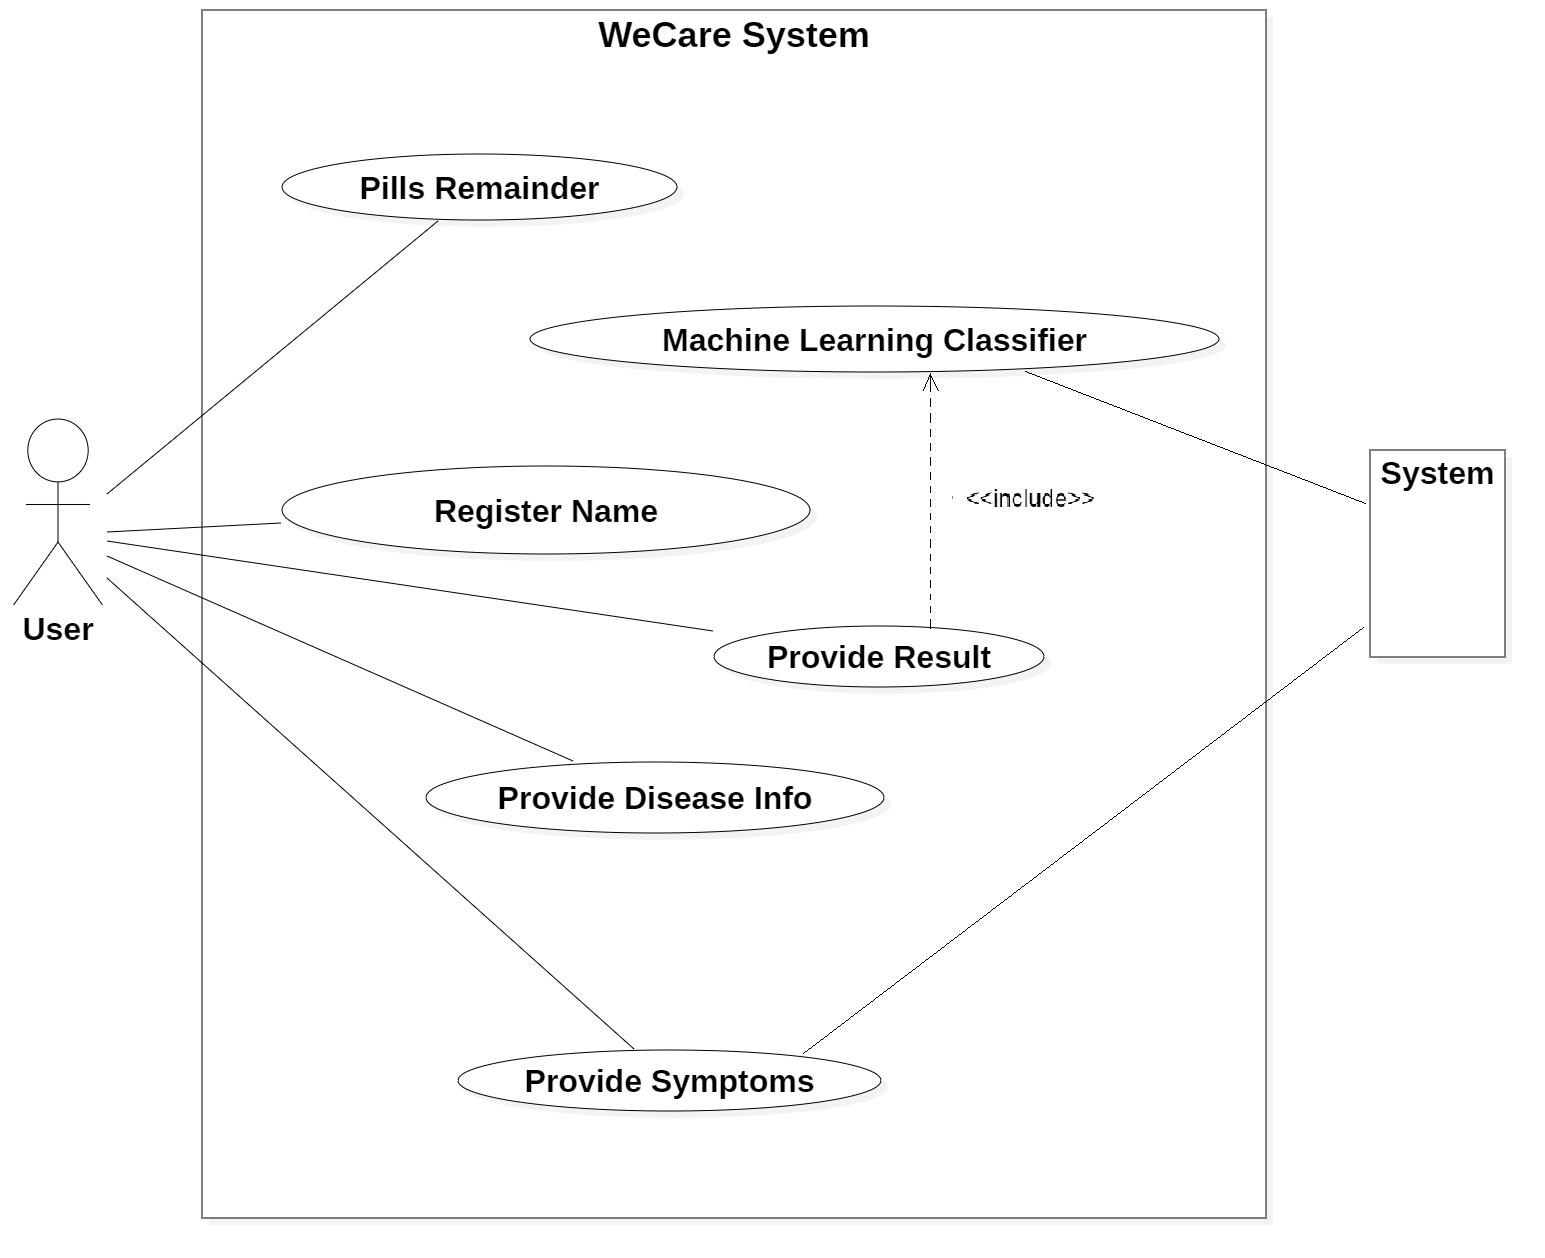
\includegraphics[width=150mm,height=170mm]{images/usecase.png}
 \caption{UseCase Diagram}
 \end{center}                
\end{figure}

\subsection{Activity diagram}
\begin{figure}[H]
\begin{center}
    
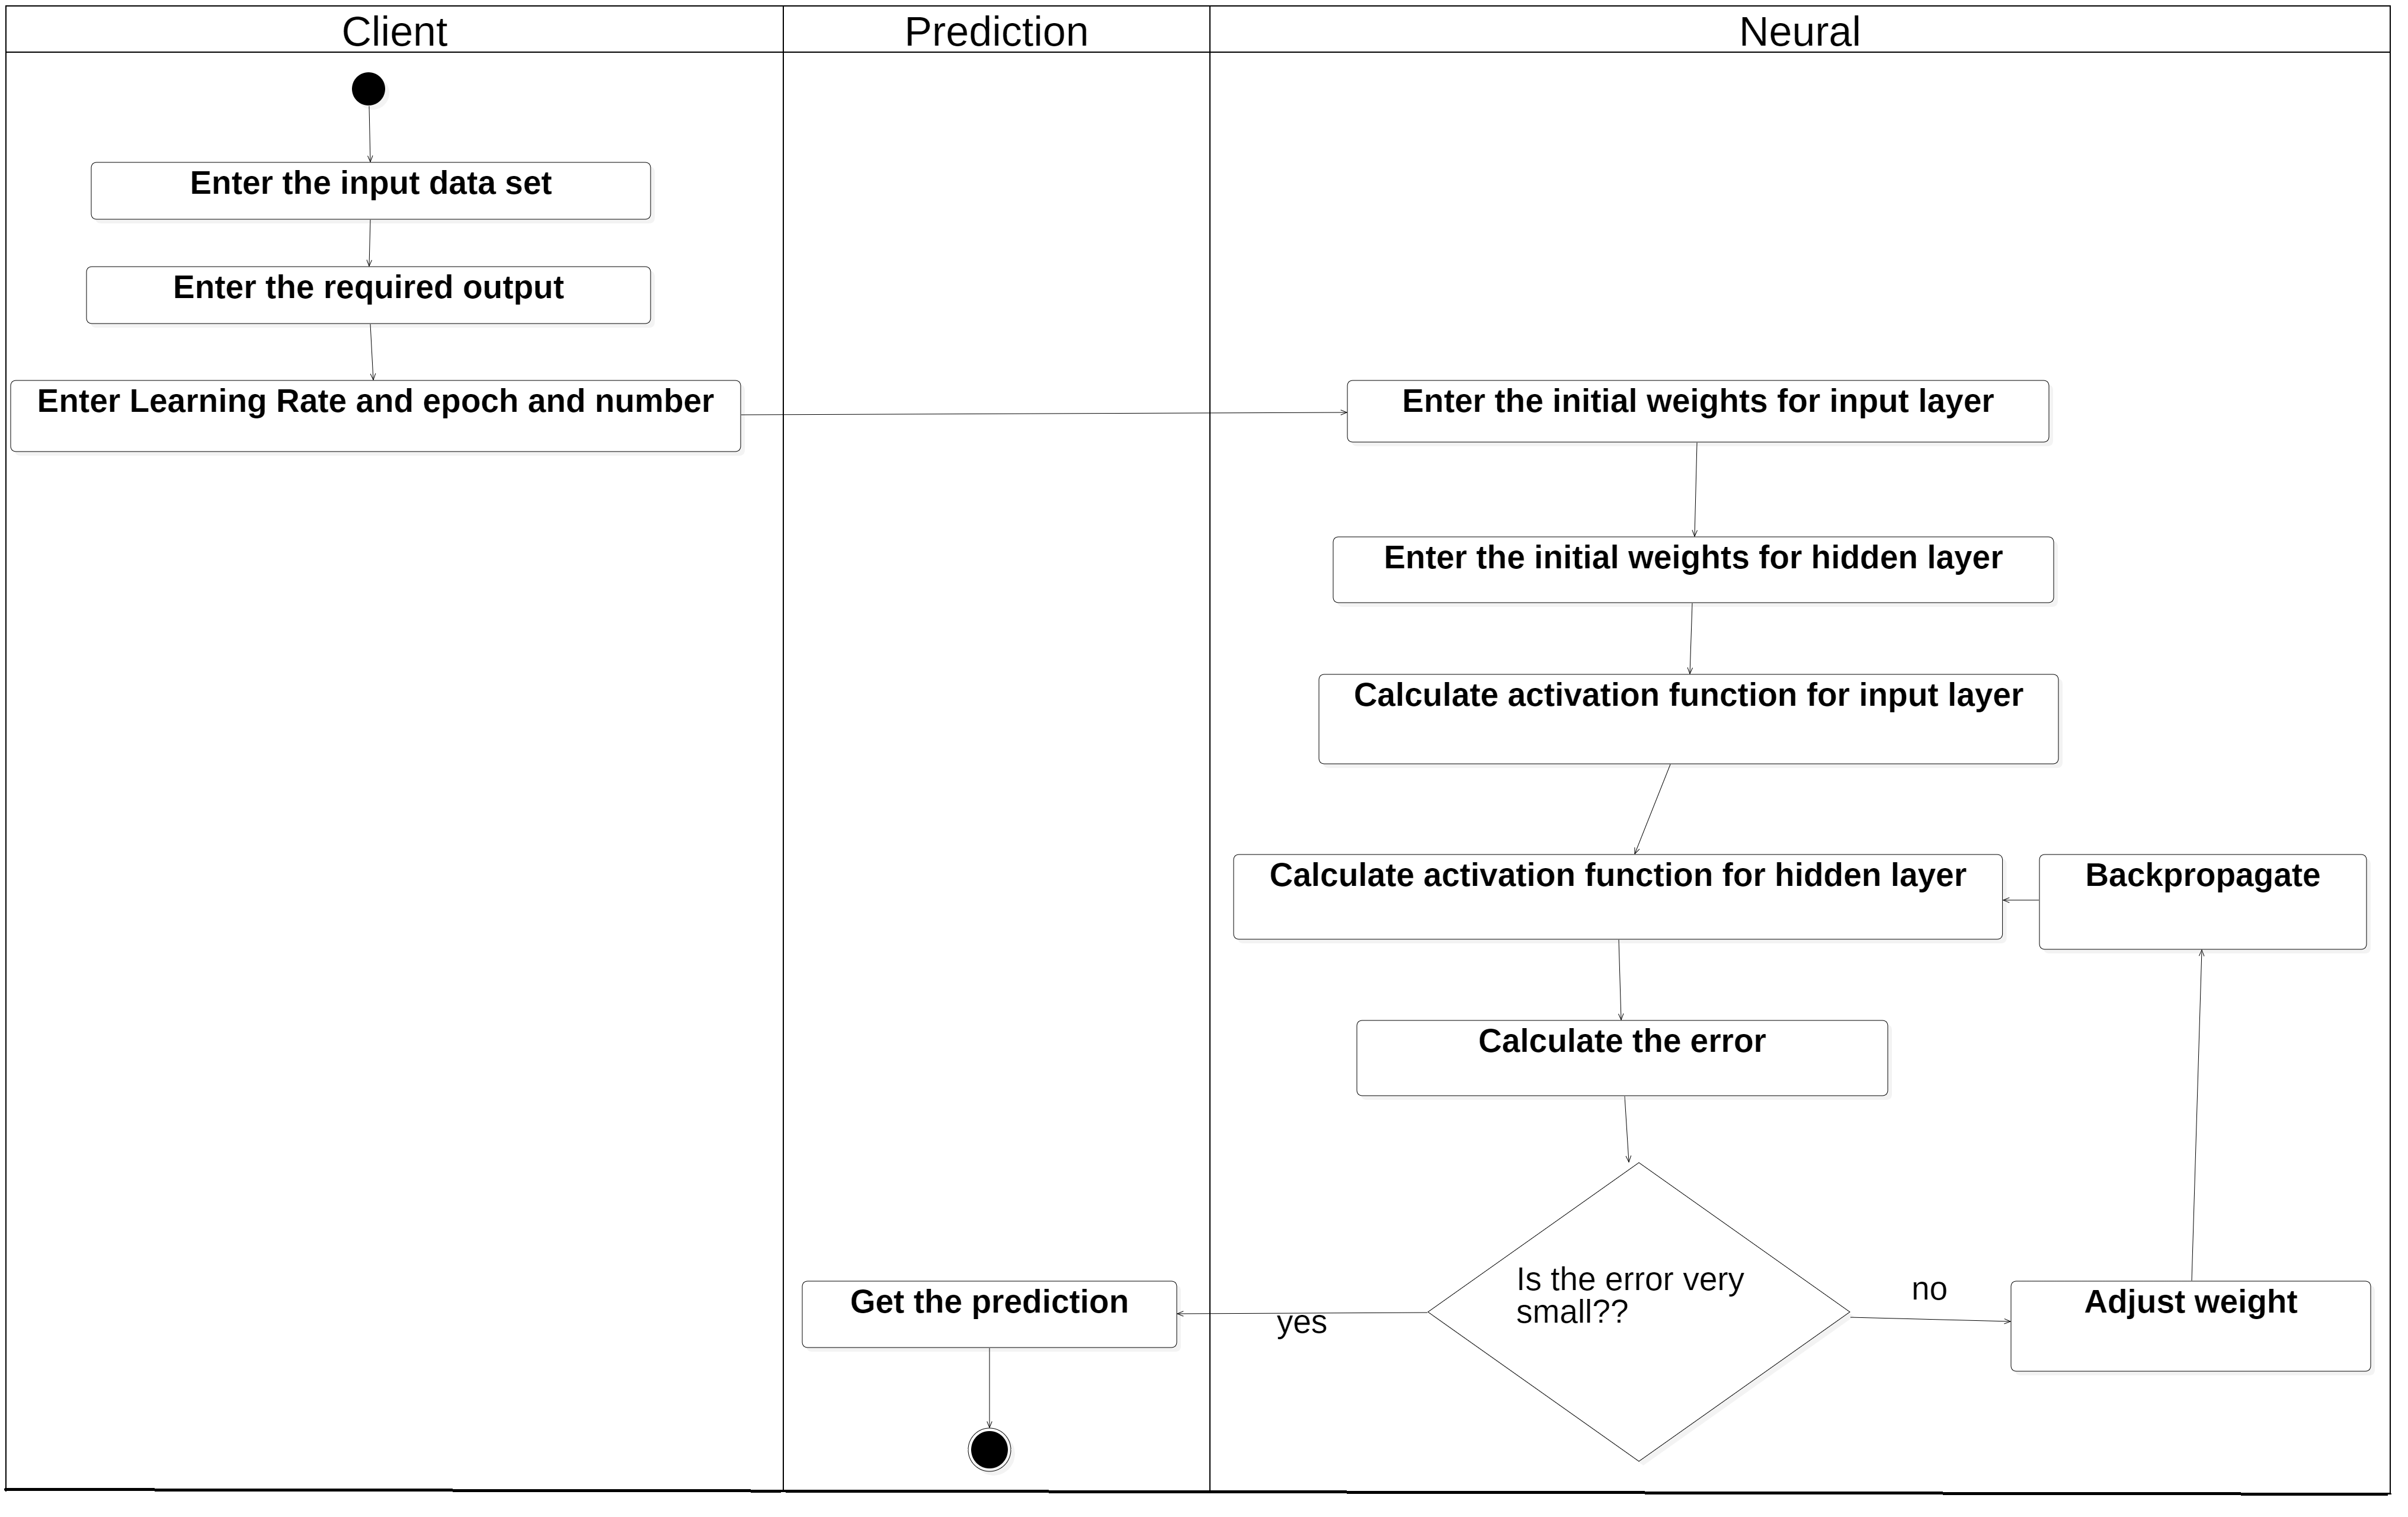
\includegraphics[width=160mm,height=175mm]{images/activity.png}
 \caption{Activity Diagram}
 \end{center}                
\end{figure}


\chapter{Epilogue}

\subsection{Designing UI prototype}
Designing UI prototype is essential steps in any project development. Designing UI prototype will gave us mockup of project we wish to build. For our UI prototyping we use Adobe XD software. We designed basic UI where user can enter their symptoms and get their result display.

\subsection{Prototype}
\begin{figure}[H]
\begin{center}
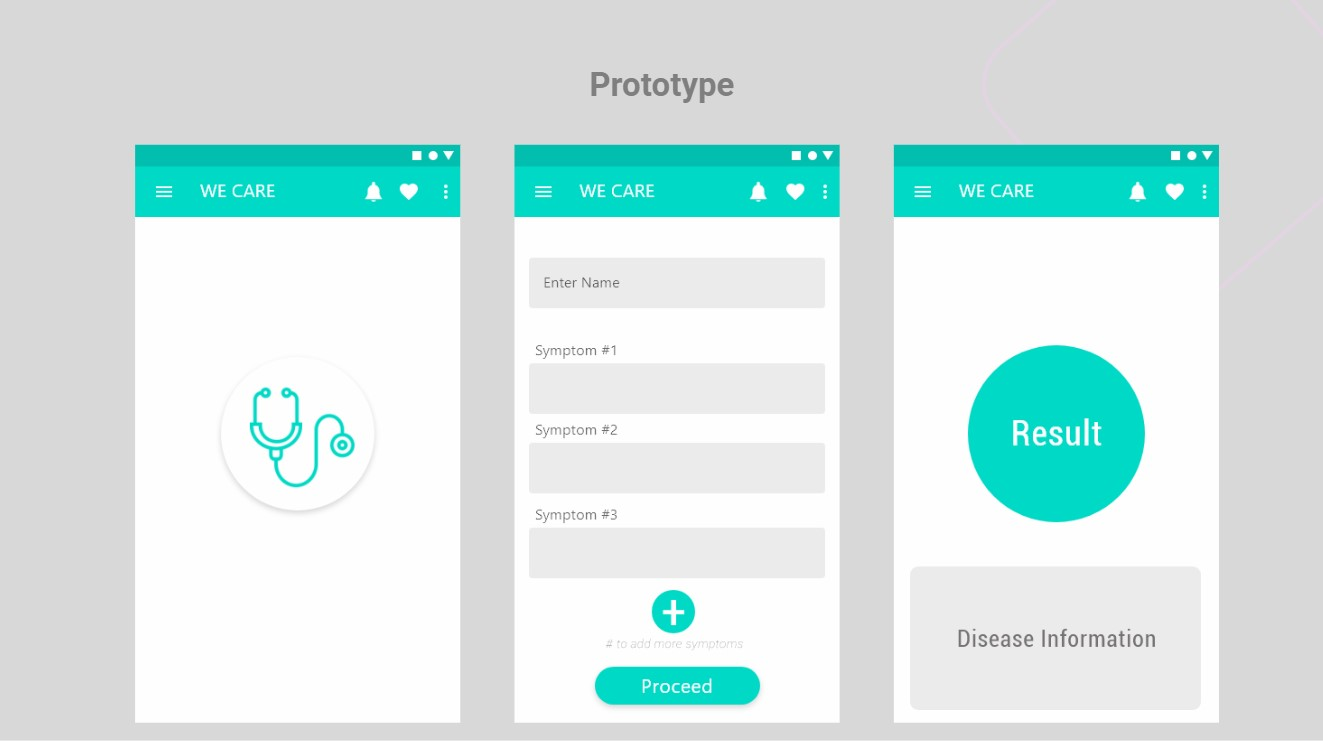
\includegraphics[width=150mm, height = 100mm]{images/prototype.jpg}
\caption{Prototype}
\end{center}
\end{figure}

\subsection{Data Collection}
Data collection is most crucial phase of any machine learning project because performance of trained model depend upon the quality of collected data sets. Finding the datasets that can be used to trained our model for solving our problem is difficult. Since our proposed system predicate the disease based on the symptoms so, we required dataset that symptoms as features and disease name as predicated class. For our project we got dataset from UCI machine learning repository and since dataset is not in format that we want so we need to format dataset as per our requirement.



\subsection{Selection of optimal Machine learning Algorithm}
Since our project is based on Classification problem, we end up with multiple good models to choose from. Each model will have different performance characteristics. The key to a fair comparison of machine learning algorithms is ensuring that each algorithm is evaluated in the same way on the same data.
Different performance metrics are used to evaluate different Machine Learning Algorithms.\newline For our project we used Confusion matrix which is  one of the most intuitive and easiest metrics used for finding the correctness and accuracy of the model. It is used for Classification problem where the output can be of two or more types of classes. The Confusion matrix in itself is not a performance measure as such, but almost all of the performance metrics are based on Confusion Matrix and the numbers inside it.\newline
\textbf{Terms associated with Confusion matrix:}
\begin{itemize}
    \item True Positives (TP): True positives are the cases when the actual class of the data point was 1(True) and the predicted is also 1(True)
    \item True Negatives (TN): True negatives are the cases when the actual class of the data point was 0(False) and the predicted is also 0(False 
    \item  False Positives (FP): False positives are the cases when the actual class of the data point was 0(False) and the predicted is 1(True)
    \item False Negatives (FN): False negatives are the cases when the actual class of the data point was 1(True) and the predicted is 0(False).
\end{itemize}

For  each  algorithm  the  accuracy, precision, sensitivity are observed which are described as follows:\newline
1.\textbf{Accuracy:} Accuracy in classification problems is the number of correct predictions made by the model over all kinds predictions made.
\[ accuracy=  \frac{(TP+TN)}{(TP+FP+TN+FN)} \]
 
2.\textbf{Precision:} This is the fraction of true positives in contrast to the overall correct results is calculated.
\[ Precision=  \frac{(TP)}{(TP+FP)} \]
 
3.\textbf{Sensitivity:} Sensitivity  is  the  true  positive  rate  and  is  defined  as  the number of positive tuples which are correctly classified.
 \[ Sensitivity=  \frac{(TP)}{(TP+FN)} \]
 

 
\begin{figure}[H]
\begin{center}
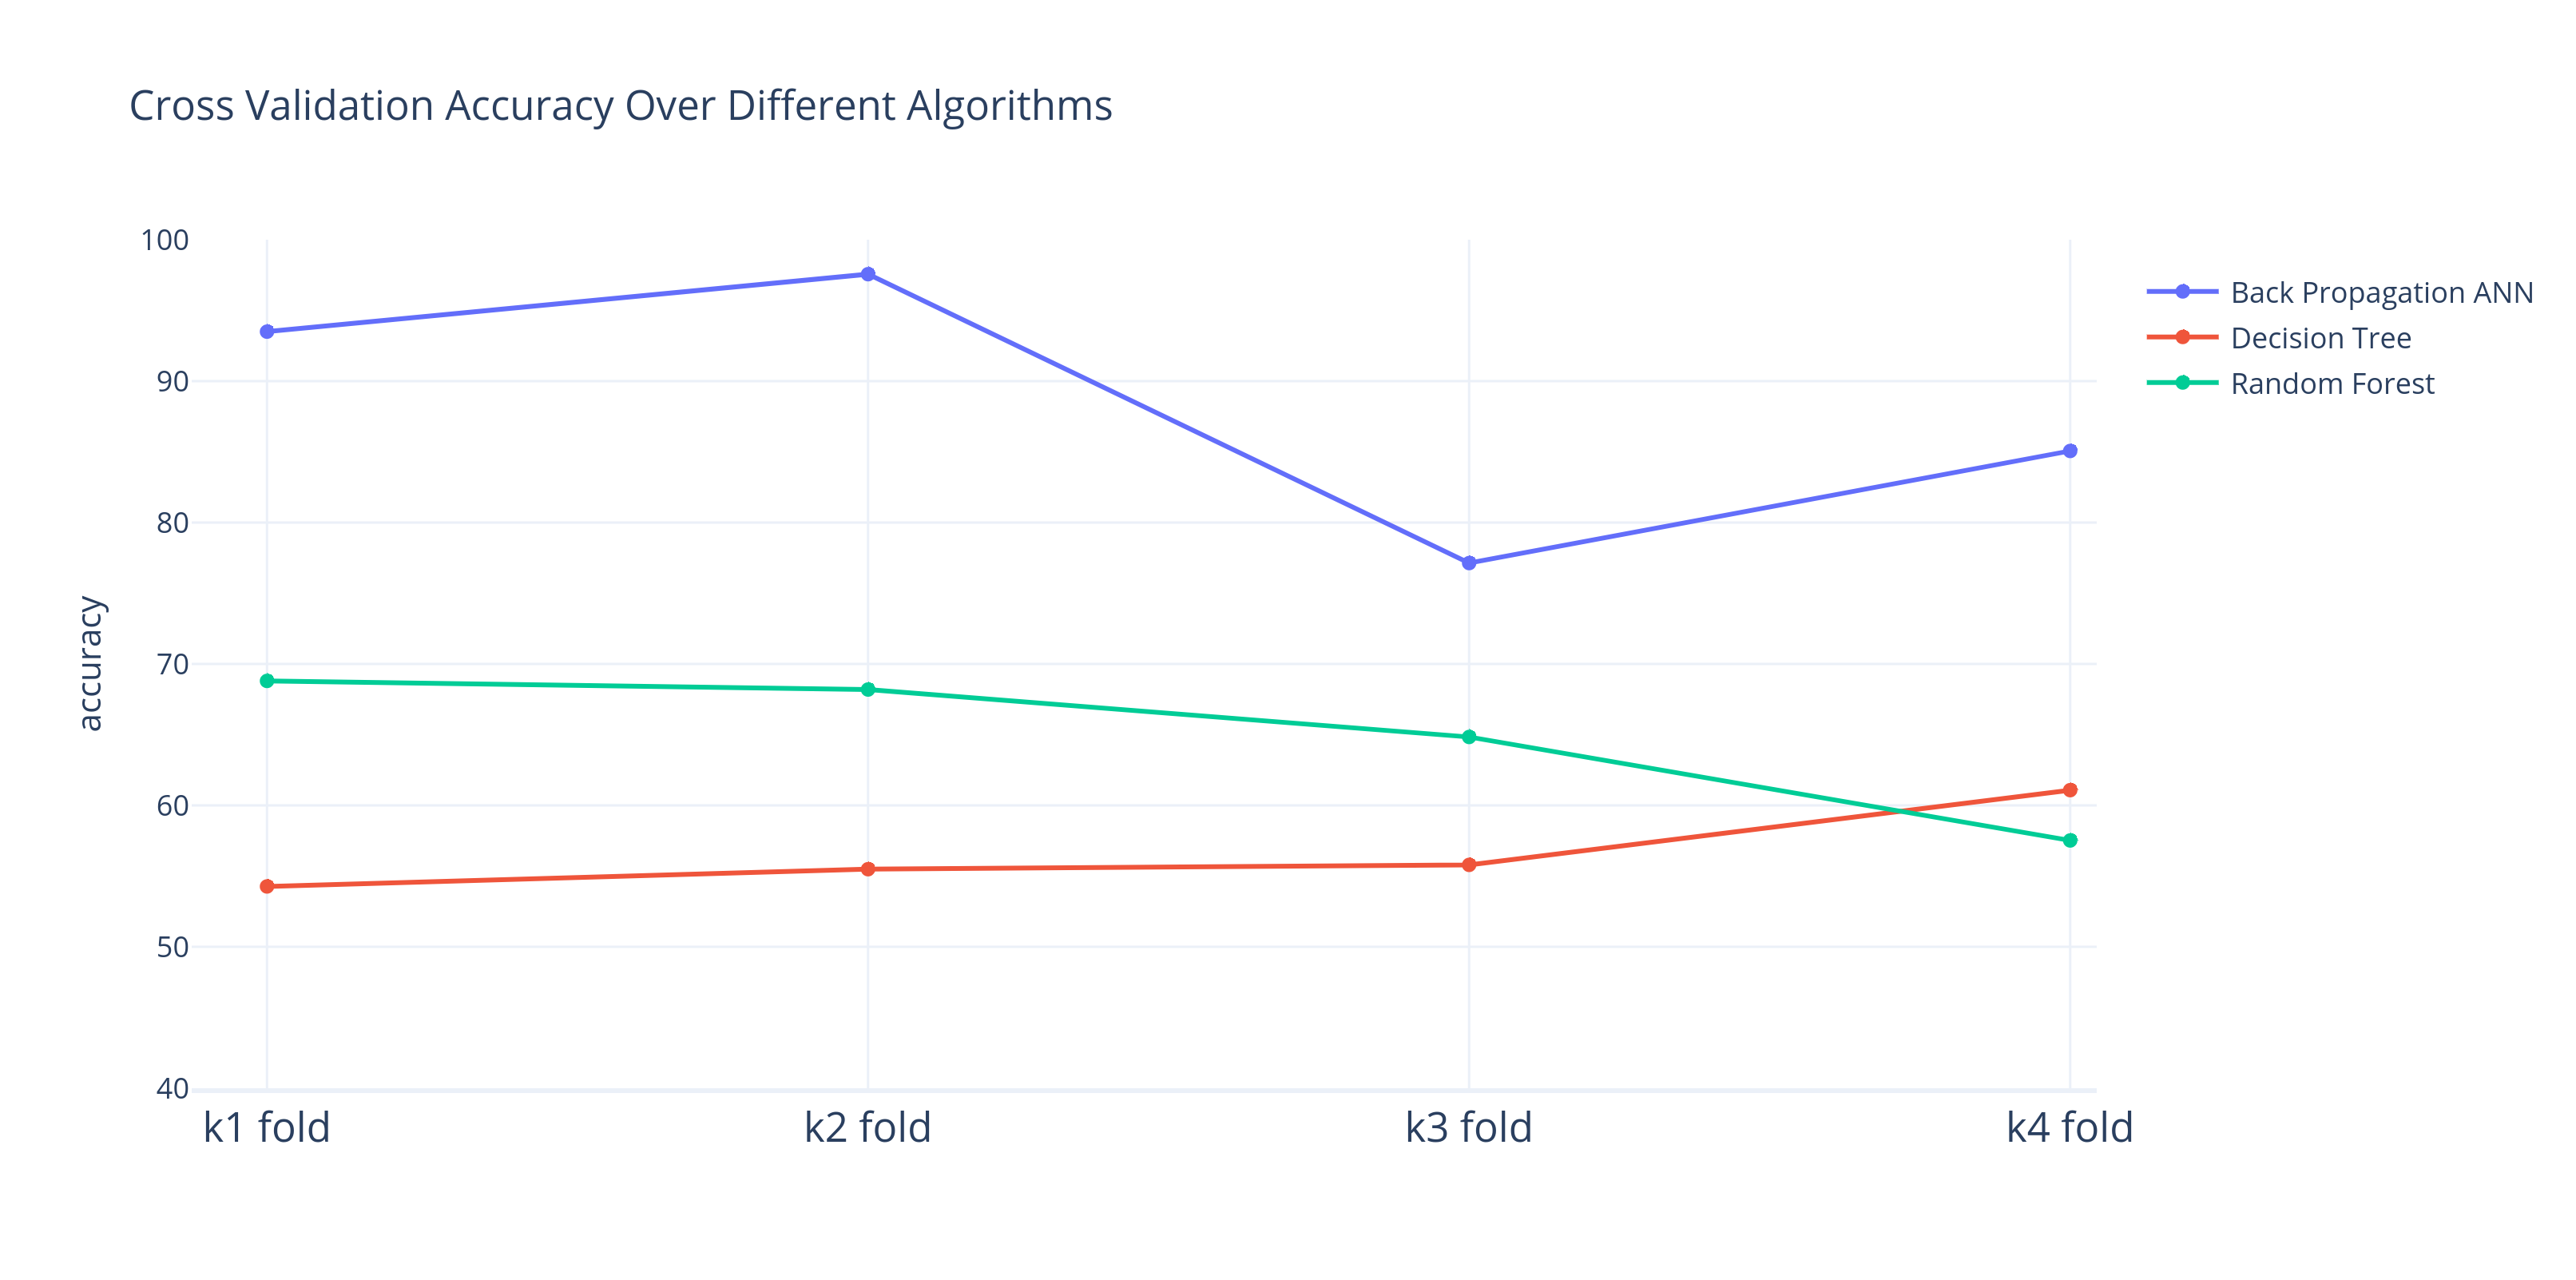
\includegraphics[width=150mm,height=90mm]{comparisonnew/accuracy.png}
 \caption{Graphical representation of accuracy}
 \end{center}                
\end{figure}
The above graph, Figure 4.2 depicts that the back Propagation ANN  have  the  highest  accuracy  when  compared  to  the other algorithms.


\begin{figure}[H]
\begin{center}
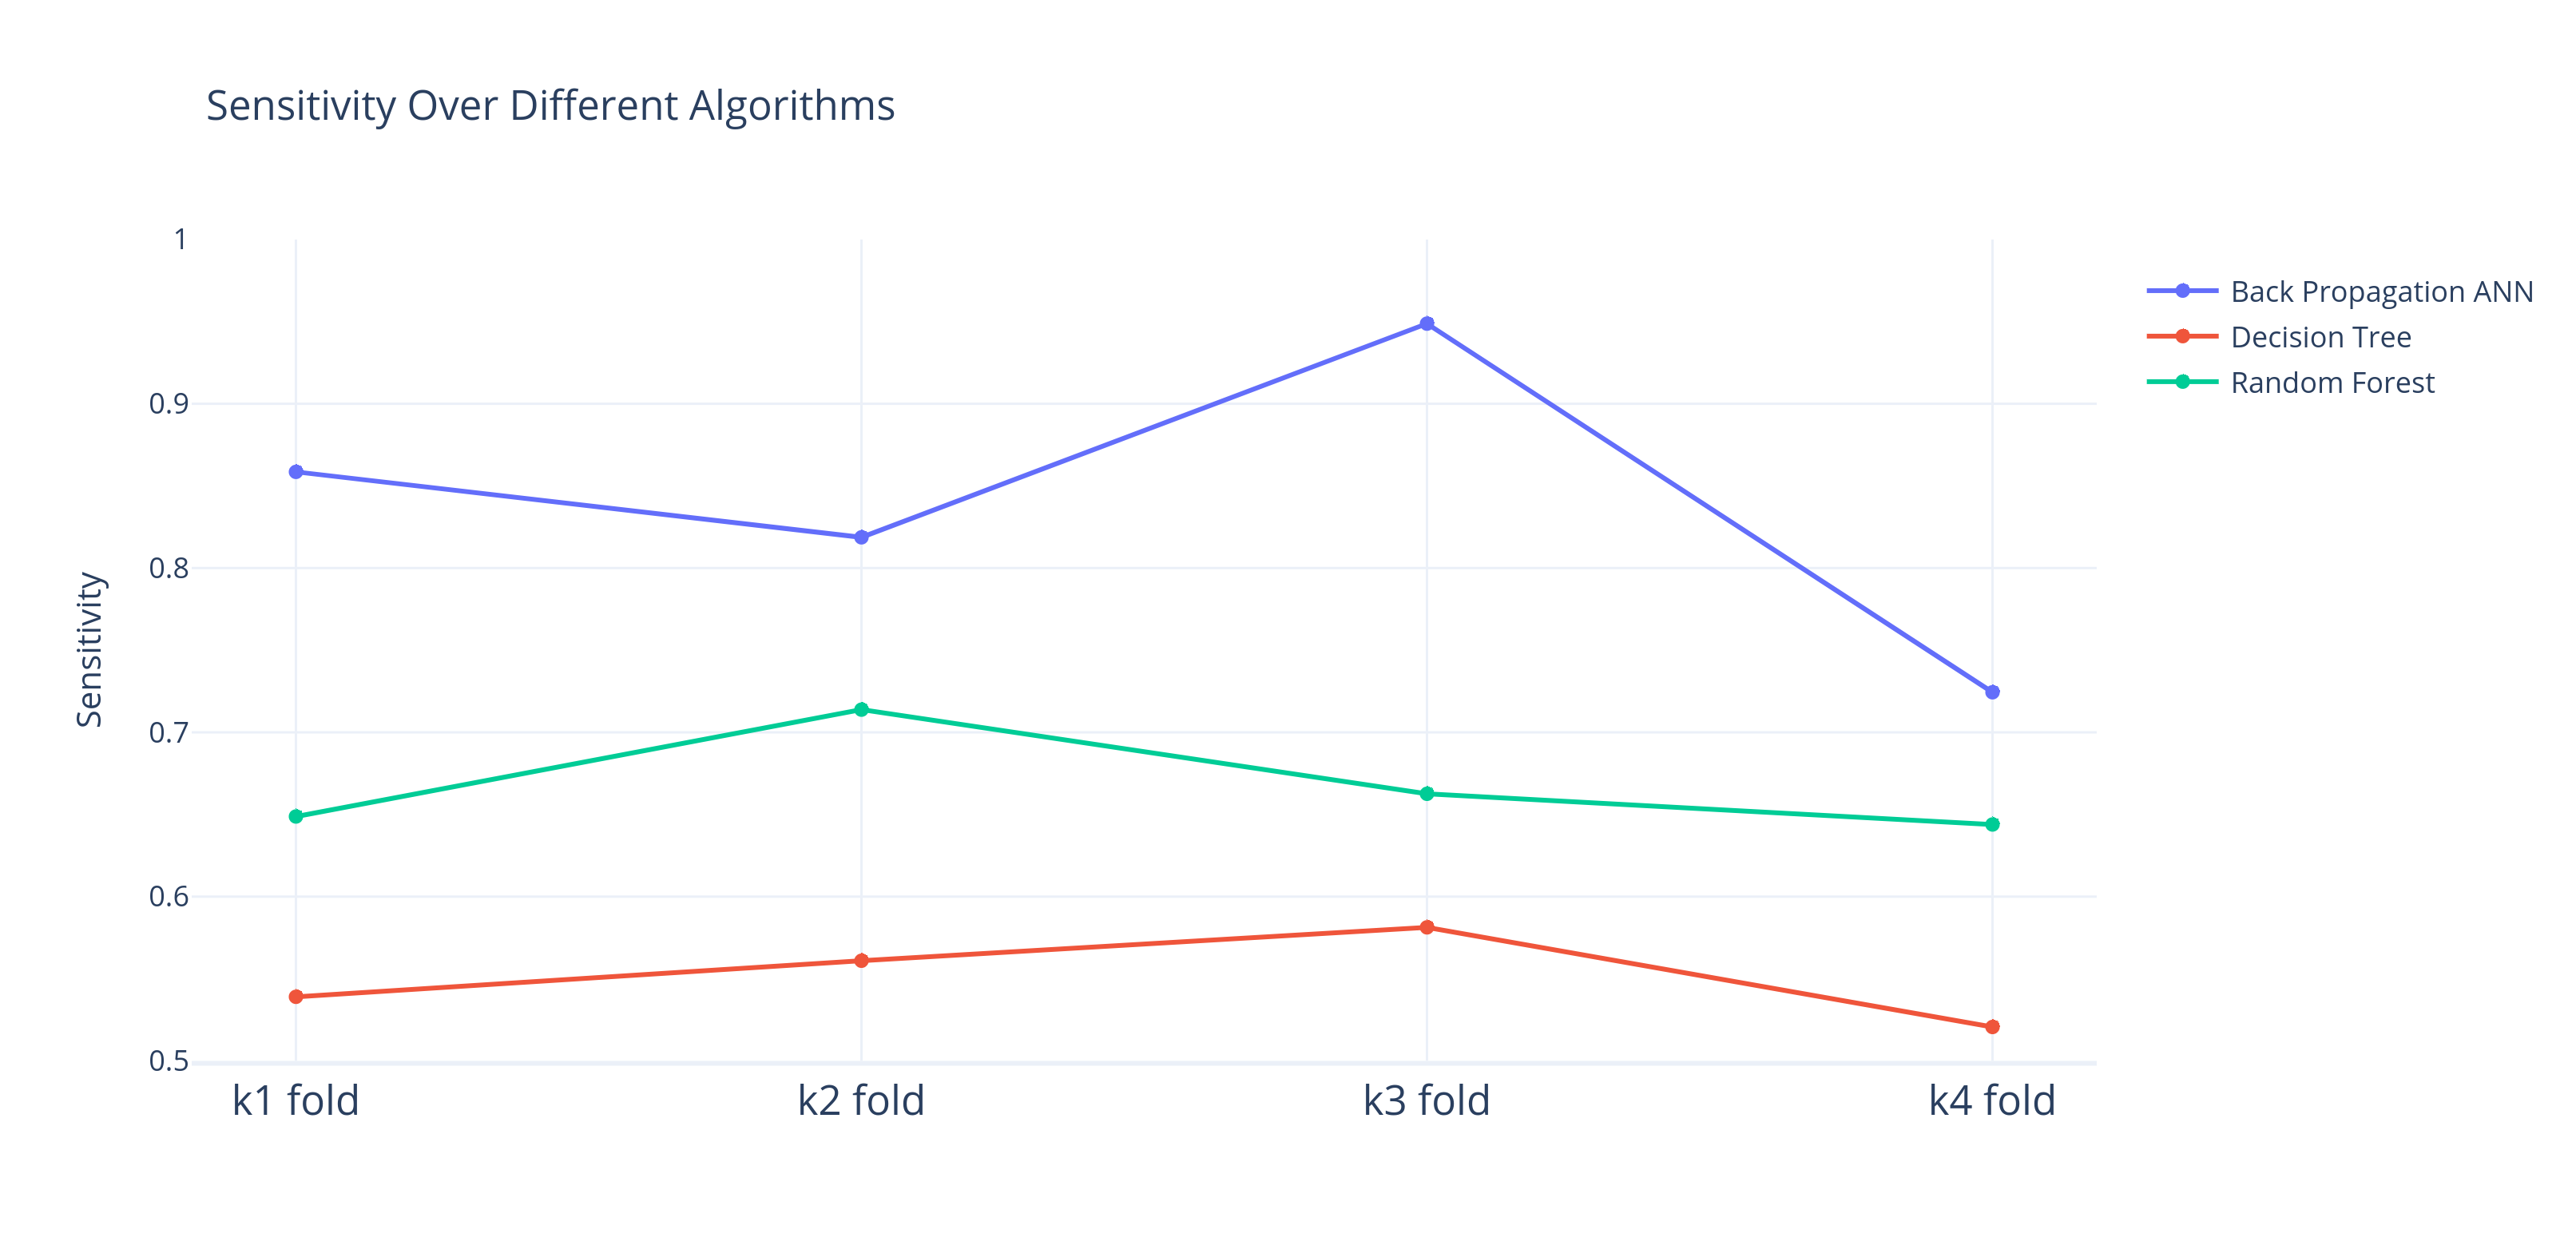
\includegraphics[width=150mm,height=90mm]{comparisonnew/sensitivity.png}
 \caption{Graphical representation of sensitivity}
 \end{center}                
\end{figure}
The   above   graph, Figure 4.3 depicts  that    back Propagation ANN  models  have the highest sensitivity.

\begin{figure}[H]
\begin{center}
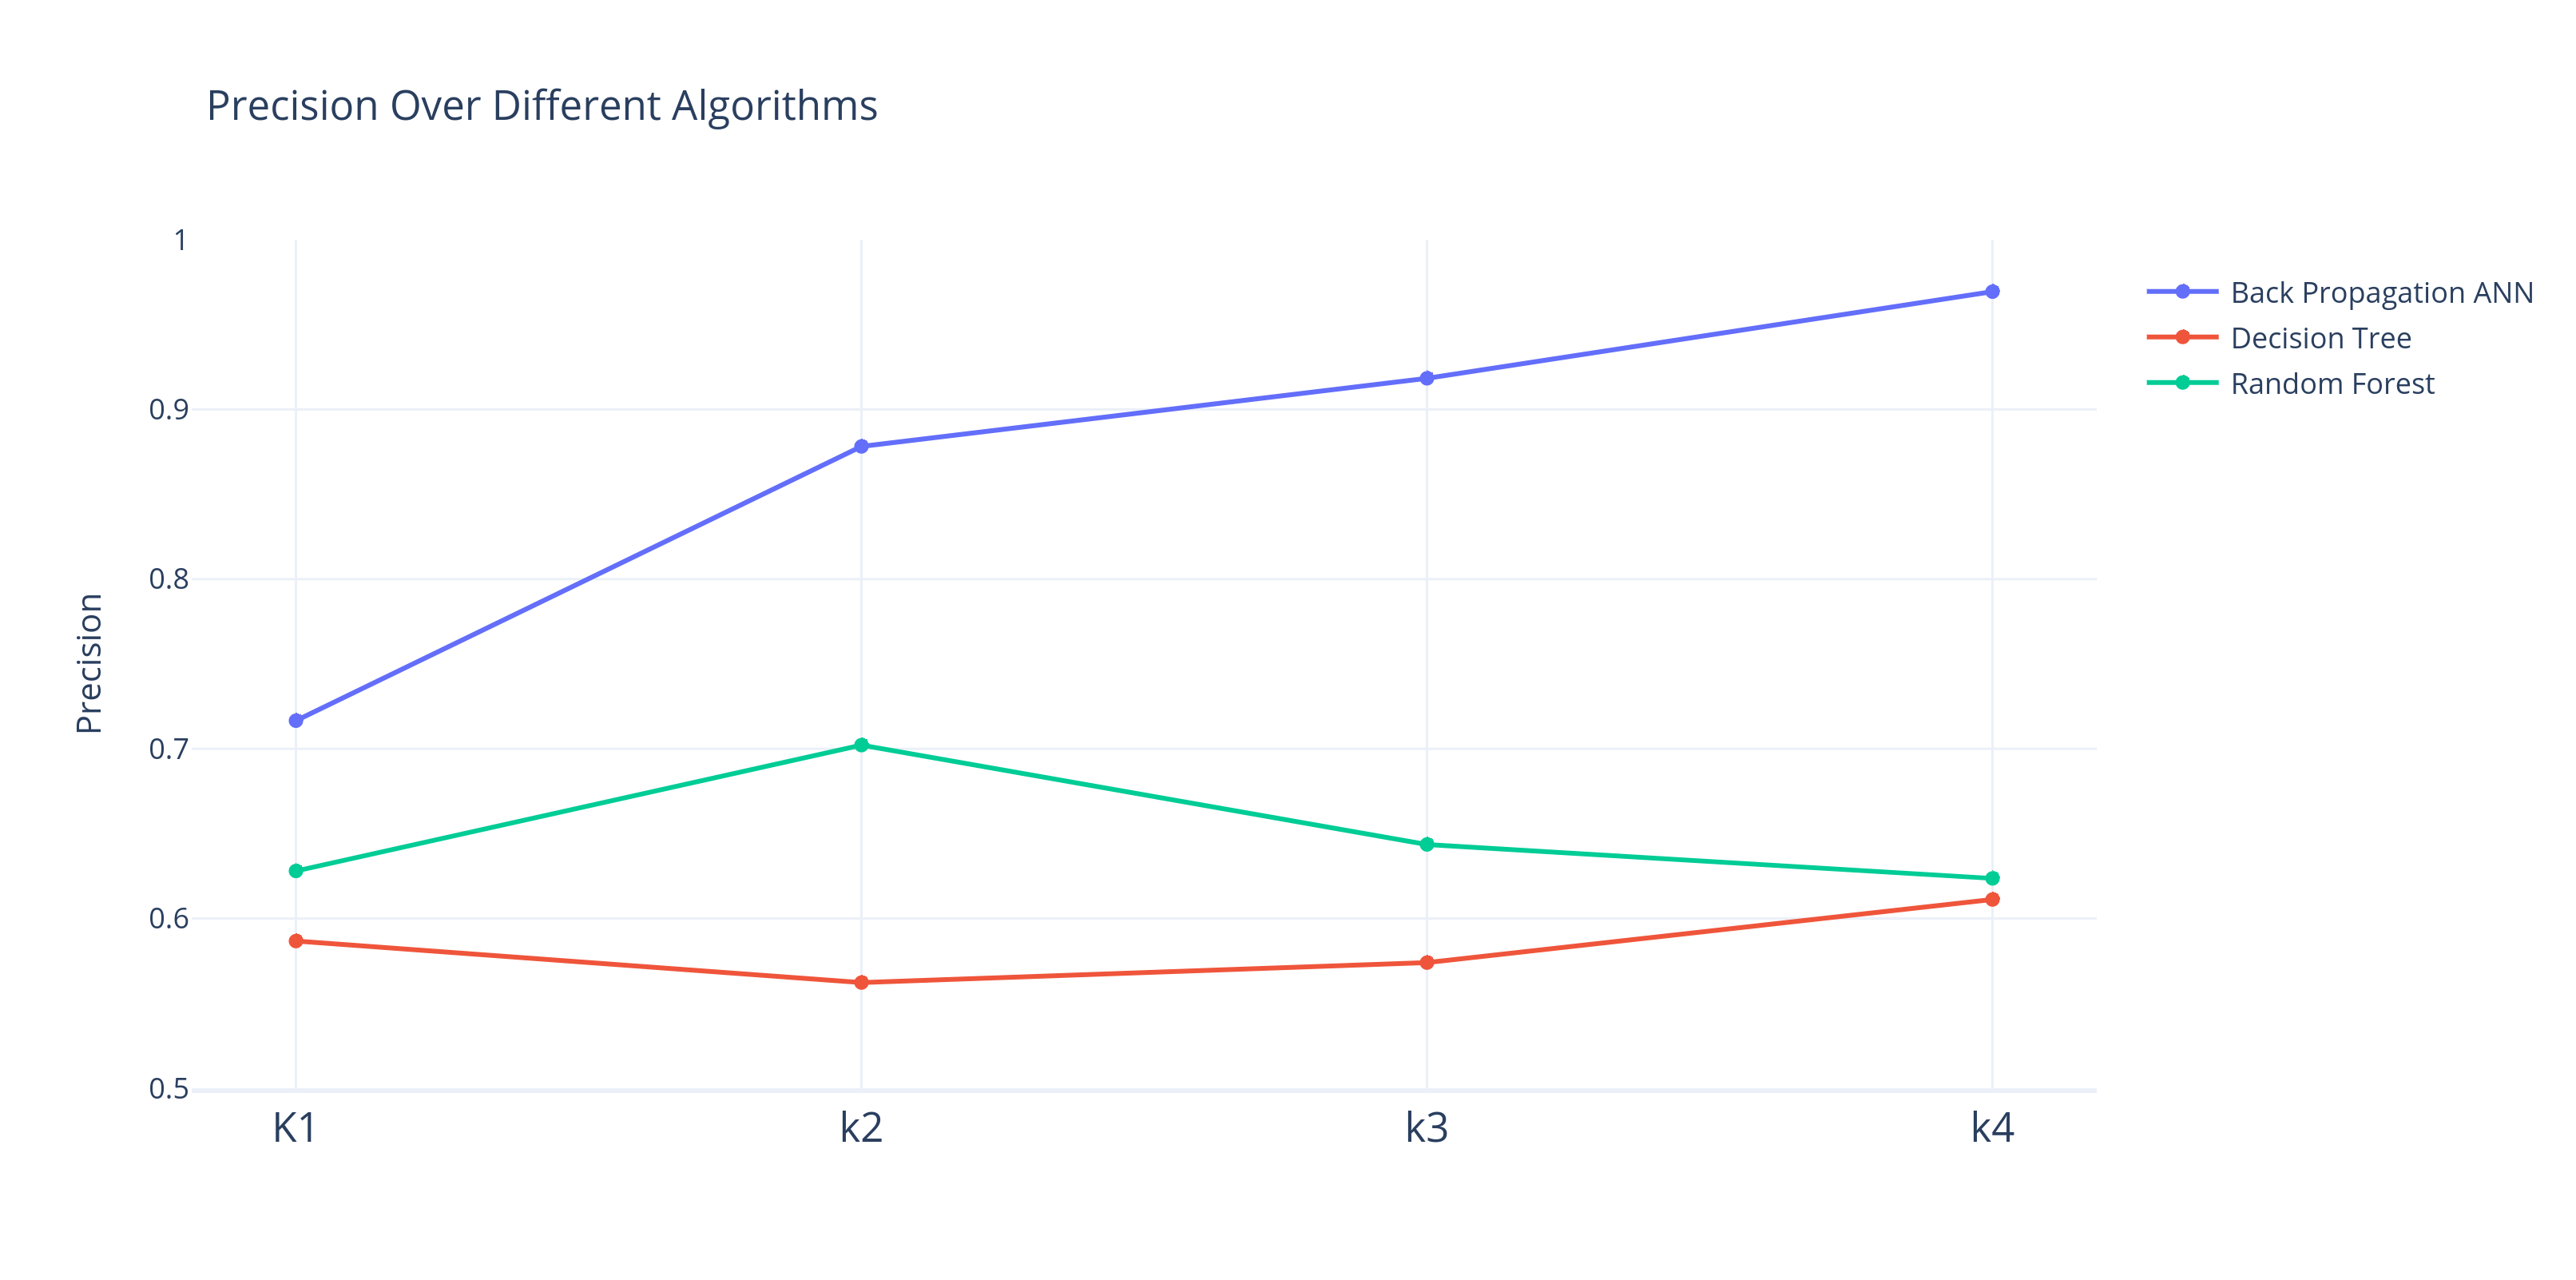
\includegraphics[width=150mm,height=90mm]{comparisonnew/precision.png}
 \caption{Graphical representation of precision}
 \end{center}                
\end{figure}

The  above  graph, Figure 4.4 depicts that back Propagation ANN  models  have the highest sensitivity.\newline

\subsection{Reason of Using Back Propagation ANN algorithm}

 From the above analysis of different classification algorithm on our dataset we conclude  that the proposed method effectively predicates the diseases when compared to the other approaches. So our proposed system is able predict the diseases with 92\% accuracy using 6 hidden layer. Our predication system gave improved result with high accuracy by using a higher number of hidden layers, but training model with higher hidden layer require a lot of computational power, so due to technical difficulty we are not able to train our model with a higher number of hidden layers.

\subsection{Selection of optimal  hyperparameter value for Modeling}

Since we are using Back Propagation Algorithm which is a supervised learning method. Before training this model we need to pass certain hyperparameter such as learning rate, epoch. Right hyper-parameters are crucial to training success.

There is no universal learning rate value which will work for all types of project. So learning rate value is highly dependent on problem at hand and in order to find suitable learning rate value for our project we explore how learning rate affect the model performance.

For this we trained our neural Network with stochastic gradient descent for different value of learning rate and Activation function such as sigmoid, relu, tanh. We used cross validation test method to determine the performance of model on different parameters and  we conclude that sigmoid activation function and learning rate=0.6 is optimal for our neural Network model as we got around 88\%  accuracy while increasing or decreasing learning rate values reduce the accuracy of model.

\begin{figure}[H]
\begin{center}
    
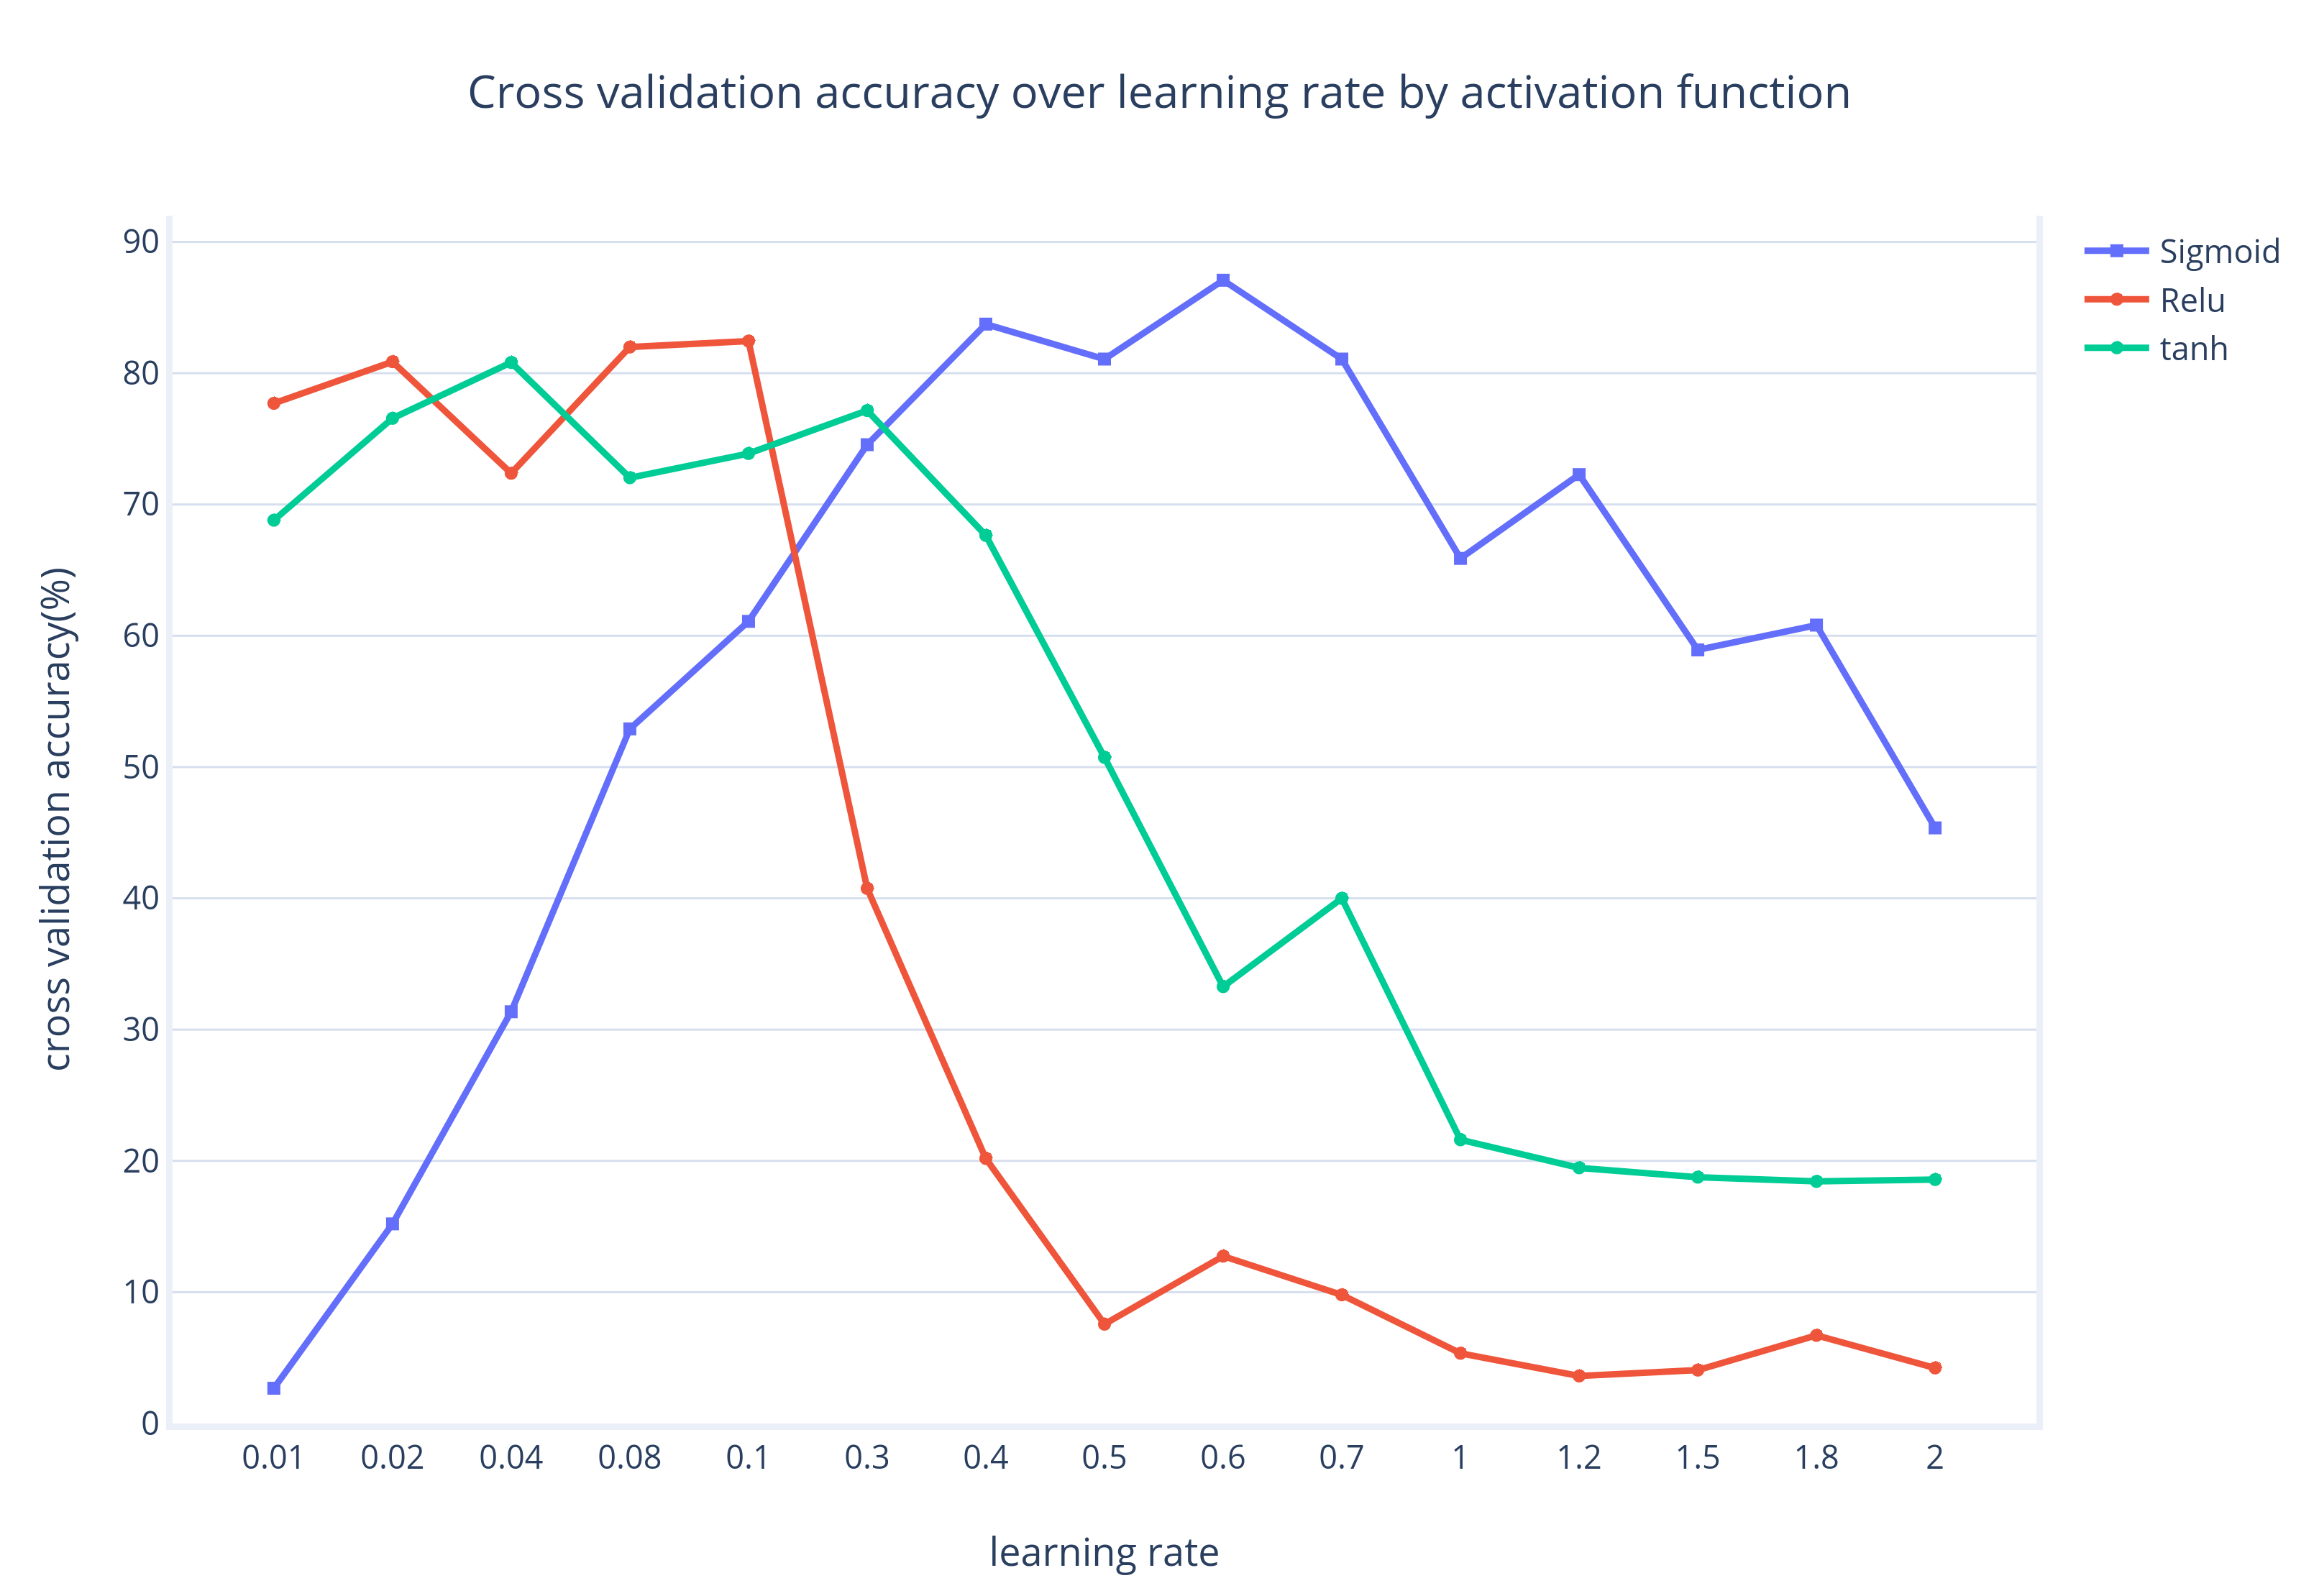
\includegraphics[width=170mm,height=120mm]{dataset_summary/selectionHyperparameter.png}
 \caption{Selection of optimal learning rate and activation function}
 \end{center}                
\end{figure}

\begin{figure}[H]
\begin{center}
    
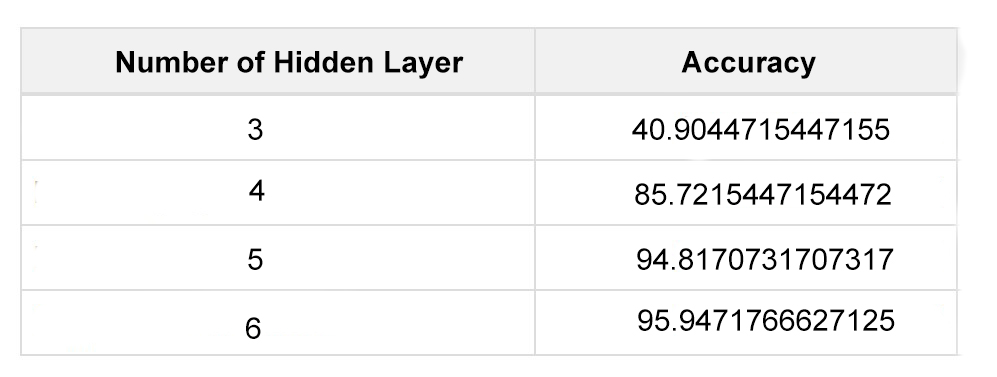
\includegraphics[width=100mm,height=50mm]{comparison/hiddenlayer.jpg}
 \caption{Selection of optimal Number of Hidden Layer}
 \end{center}                
\end{figure}


At the beginning of the project, we trained data with 3 hidden layers which took 3 hours and gave 40.98 \% accuracy which was not applicable to predict the disease and get optimal result.
Due to unsatisfactory result, we again trained with 4 hidden layers which took 6 hours and gave 85.72 \% accuracy which was applicable but not satisfactory as per our expectation and to predict the disease and get optimal result.
We again trained with 5 hidden layers which took 14 hours and gave 94.81 \% accuracy which was much satisfactory result. Inorder to obtain little more accuracy we tried to trained with 6 hidden layers which eventually took 24 hours and gave 95.94 \% which is high accuracy than previous hidden layers but it limits our computer system and to evaluate 6 hidden layers our computer system gets heated and had to resume training many time. \par
So, we stopped due to our system failure and limitation. At last we concluded to train data with 6 hidden layers and 95.94 \% accuracy to predict the disease and get optimal result. 
Another reason for not increasing hidden layer size from 6 is since our dataset is relatively small and increasing the hidden layer will cause our model to be overfitted to our dataset and hence reduce accuracy.




\subsection{Back Propagation Algorithm implementation using Python}

1. \textbf{Initialize Network:}
Each neuron has a set of weights that need to be maintained. One weight for each input connection and an additional weight for the bias. We will need to store additional properties for a neuron during training, therefore we will use a dictionary to represent each neuron and store properties by names such as ‘weights‘ for the weights.
Initially, we randomly set the weights of neuron.\newline
Function named initialize\_network that creates a new neural network ready for training. It accepts three parameters, the number of inputs, the number of  hidden layer and the number of outputs.\newline
Each neuron  has n\_inputs + 1 weights, one for each input column in a dataset and an additional one for the bias.

\begin{figure}[H]
\begin{center}
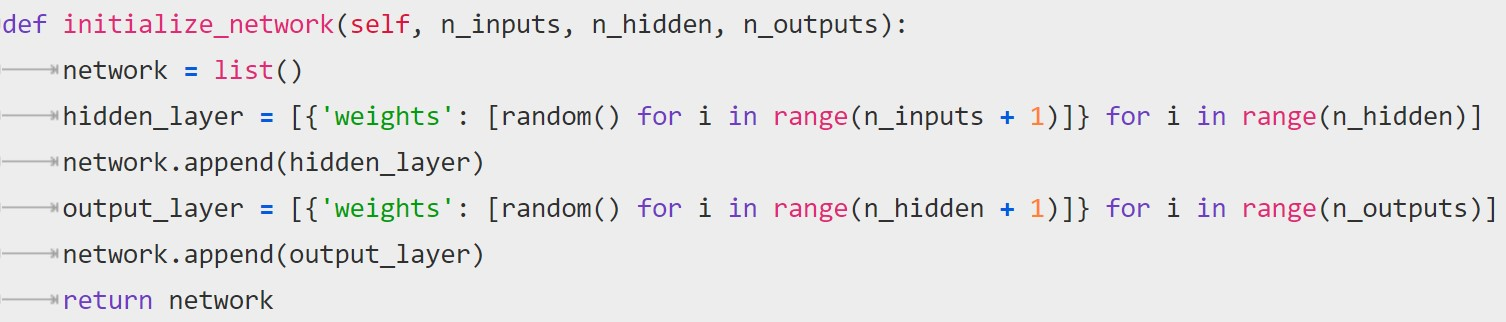
\includegraphics[width=160mm,height=45mm]{backexplain/initializeNetwork.jpg}
\end{center}
\end{figure}

2. \textbf{Forward Propagate:}
We can calculate an output from a neural network by propagating an input signal through each layer until the output layer outputs its values.
We call this forward-propagation.\newline
Forward propagation down into three parts:\newline
    1.Neuron Activation.\newline
    2.Neuron Transfer.\newline
    3.Forward Propagation.\newline
    
2.1 \textbf{Neuron Activation}
The first step is to calculate the activation of one neuron on given an input.\newline
Neuron activation is calculated as\newline
           \centerline{activation= sum(weight*input)+bias }

\begin{figure}[H]
\begin{center}
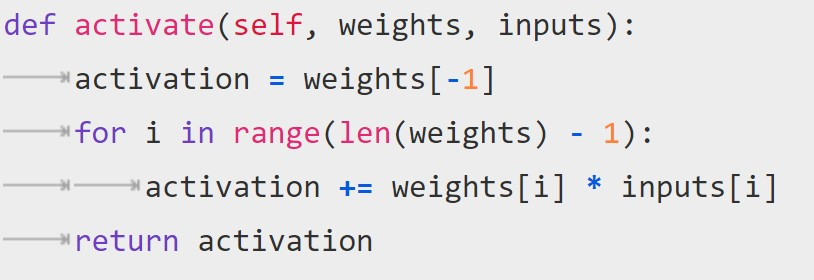
\includegraphics[width=120mm,height=40mm]{backexplain/activate.jpg}
\end{center}
     
\end{figure}            
            


2.2 \textbf{Neuron Transfer}
Once a neuron is activated, we need to transfer the activation to see what the neuron output actually is.
There are different transfer function but for our project we used Sigmoid Activation function.\newline
The sigmoid activation function looks like an S shape, it’s also called the logistic function. It can take any input value and produce a number between 0 and 1 on an S-curve. It is also a function of which we can easily calculate the derivative (slope) that we will need later when backpropagating error.
\newline
Output of neuron using sigmoid activation function \newline
{output=1/(1+ exp^{-activation})

Below is a function named transfer that implements the sigmoid equation.

\begin{figure}[H]
\begin{center}
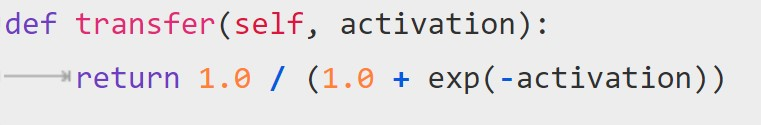
\includegraphics[width=110mm,height=20mm]{backexplain/transfer.jpg}
\end{center}
     
\end{figure} 

2.3 \textbf{Forward Propagation}
output of each neurons is calculate and output of one neurons become input to another neurons.\newline
Function named forward\_propagate (\,)\, that implements the forward propagation for a row of data from our dataset with our neural network.
Neuron’s output value is stored in the neuron with the name "output". We collect the outputs for a layer in an array named new\_inputs that becomes the array inputs and is used as inputs for the following layer.

\begin{figure}[H]
\begin{center}
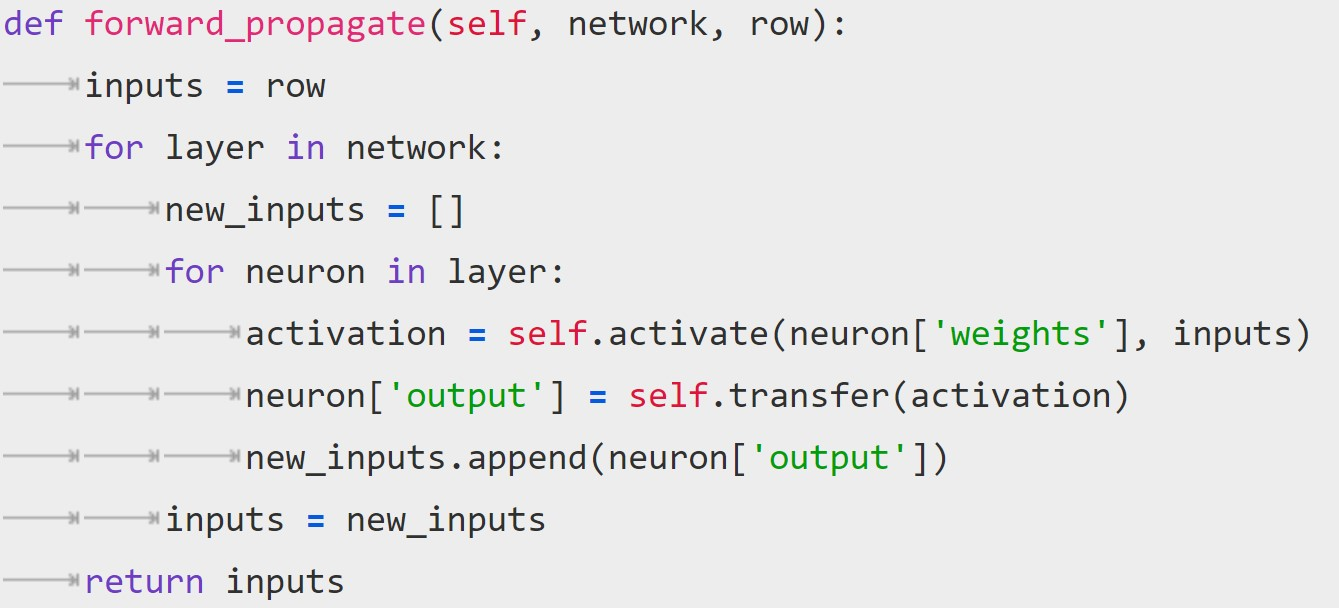
\includegraphics[width=160mm,height=75mm]{backexplain/forward.jpg}
\end{center}
\end{figure} 

3. \textbf{Back Propagate Error}\newline
Error is calculated between the expected outputs and the outputs forward propagated from the network. These errors are then propagated backward through the network from the output layer to the hidden layer, assigning blame for the error and updating weights as they go.\newline
 This part is broken down into section\newline
 1. Transfer derivative\newline
 2. Error backpropagation
 
 3.1 \textbf{Transfer derivative}\newline
 Given an output value from a neuron, we need to calculate it’s slope. We are using the sigmoid transfer function, the derivative of which can be calculated as follows:\newline
        derivative = output * (1.0 - output)\newline
 Below is a function named transfer\_derivative that implements this equation:
 \begin{figure}[H]
\begin{center}
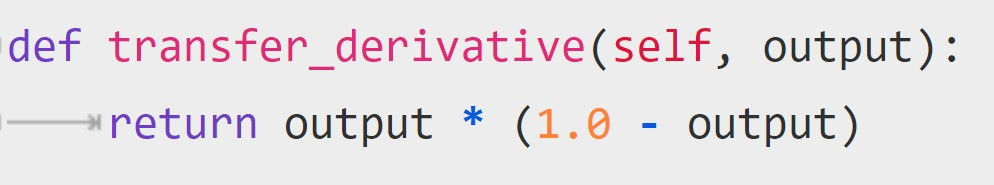
\includegraphics[width=110mm,height=20mm]{backexplain/transferDerivative.jpg}
\end{center}
\end{figure} 

\pagebreak
3.2 \textbf{Error BackPropagation:}\newline
Here we first calculate the error of each neurons, this will give error signal(input) to propagate backward through the network.\newline
The error of neuron can be calculate as:\newline
 \centerline{error=(expected-output)*transfer\_derivatives(output)}
where,\newline
expected:Expected value of neuron \newline 
output:Output value of neuron\newline
transfer\_derivate():calculates the slope of the neuron’s output value

This error calculation is used for neuron in output layer and error calculation for hidden layers is bit different and complicated then output layer.\newline The back-propagated error signal is accumulated and then used to determine the error for the neuron in the hidden layer, as follows:\newline
           \centerline{error = (weight\_k * error\_j) * transfer\_derivative(output)}
Where error\_j is the error signal from the jth neuron in the output layer, weight\_k is the weight that connects the kth neuron to the current neuron and output is the output for the current neuron.

 \begin{figure}[H]
\begin{center}
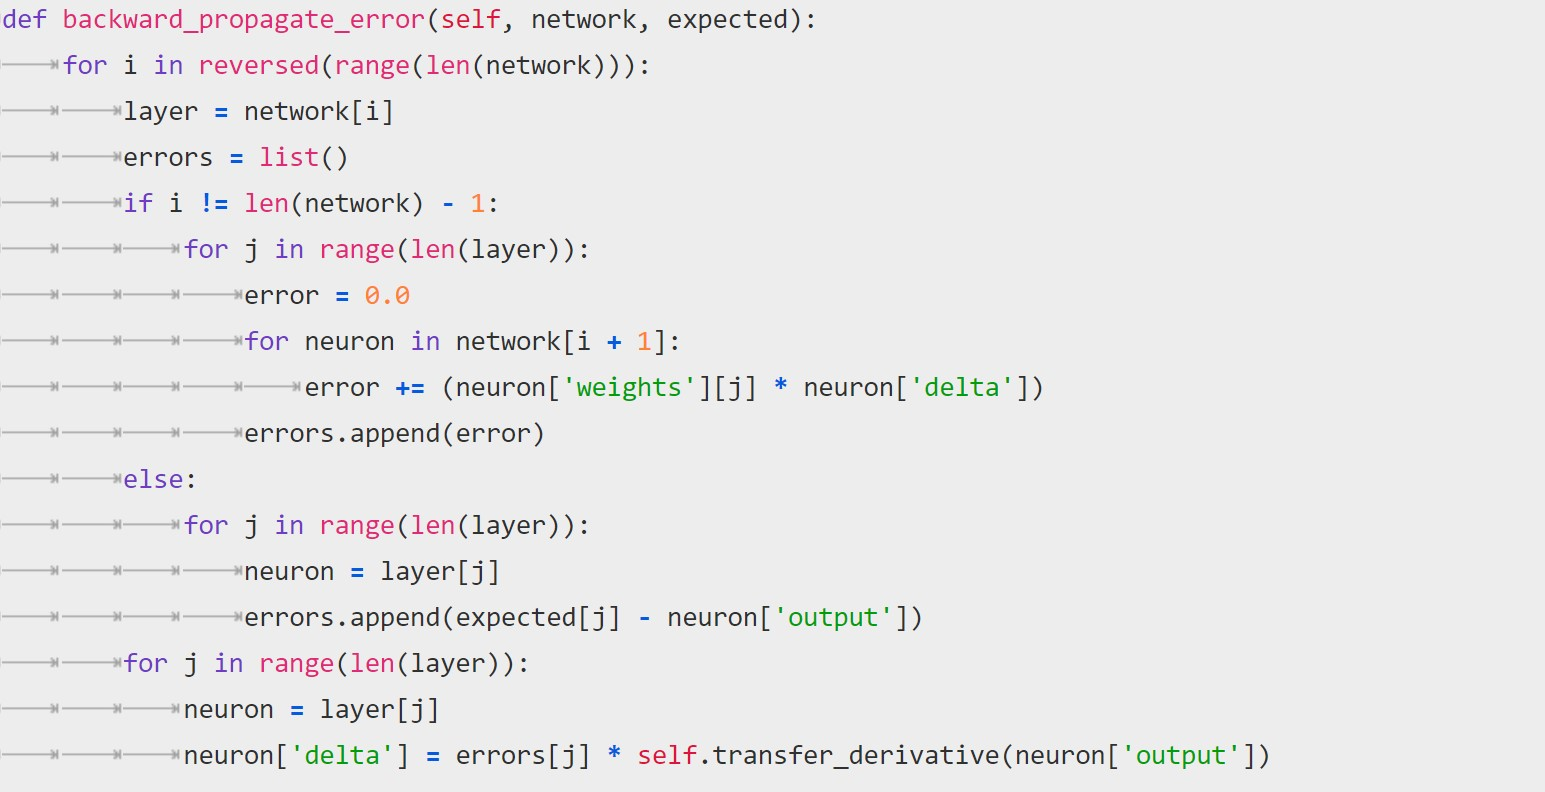
\includegraphics[width=160mm,height=100mm]{backexplain/errorback.jpg}
\end{center}
\end{figure} 

Here the error signal calculated for each neuron is stored with the name ‘delta’. The layers of the network are iterated in reverse order, starting at the output and working backwards. This ensures that the neurons in the output layer have ‘delta’ values calculated first that neurons in the hidden layer can use in the subsequent iteration.


4 \textbf{Train Network}
Here we train our network will training datasets and for each row data we propagate the data, back propagate error and update the weights.
 This part is broken down into section\newline
1. Update weights\newline
2. Train network


4.1 \textbf{Update weights}
Once errors are calculated for each neuron in the network via the back propagation method above, they can be used to update weights.\newline
Network weights are updated as follows:\newline
\centerline{weight = weight + learning\_rate * error * input}
Where weight is a given weight, learning\_rate is a hyperparameter we specify, error is the error calculated by the backpropagation procedure for the neuron and input is the input value that caused the error.
The same procedure can be used for updating the bias weight, except there is no input term, or input is the fixed value of 1.0.

\subsection{RESTFul API using Flask}

After training our neural network model we saved our neural network, which is the collection weights value of different layer of the network. Then we create a RESTful API (application program interface) which allow users to send their symptoms in HTTP request and get a response back in JSON format.

\begin{figure}[H]
\begin{center}
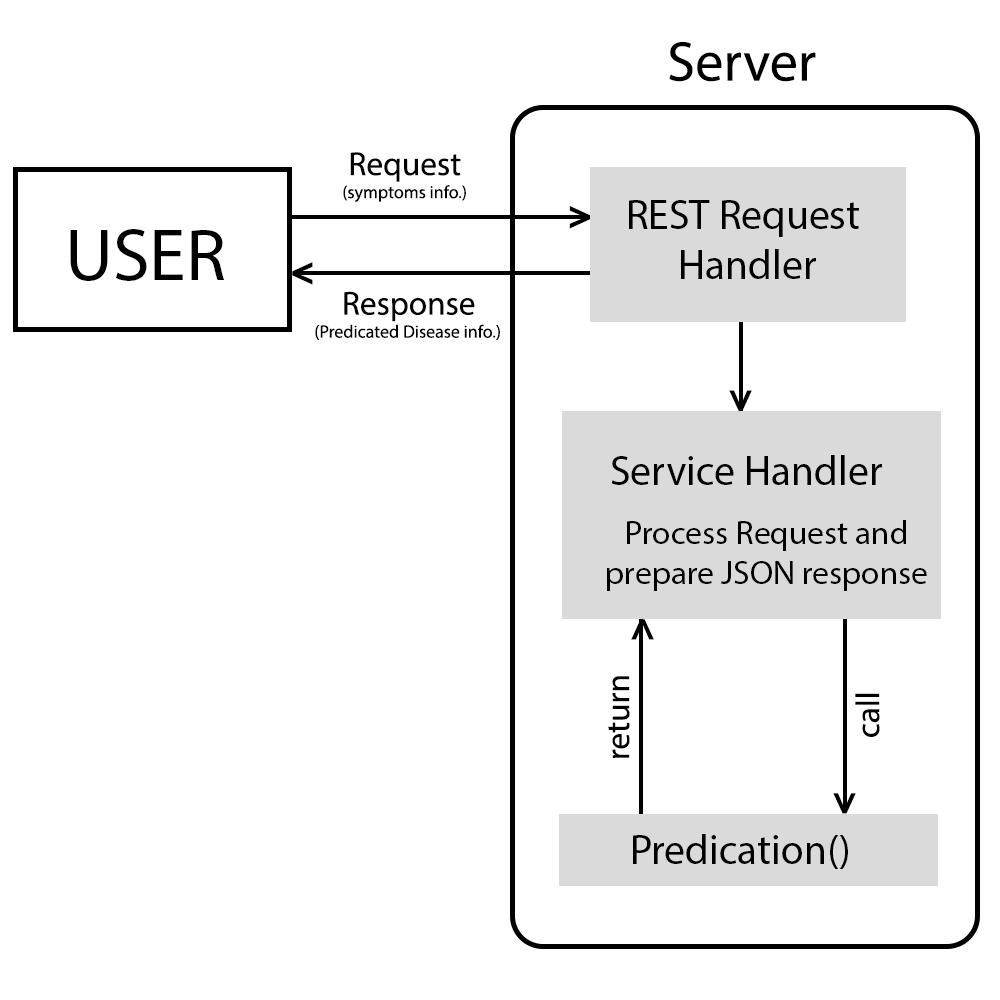
\includegraphics[width=130mm, height = 130mm]{images/restapi.png}
\caption{Restful API}
\end{center}
\end{figure}

In order to create RESTFul API we used flask in server side which is micro framework because it does not require particular tools or libraries. After that we have created route which will listen to certain HTTP request. This allowed user to send their symptoms information via HTTP request and route function will parse the data (symptoms information) from the HTTP request. Then we call predication function which neural network model, symptoms as parameters and return predicated disease information back to user.

\subsection{Output}


\begin{figure}[H]
\begin{center}
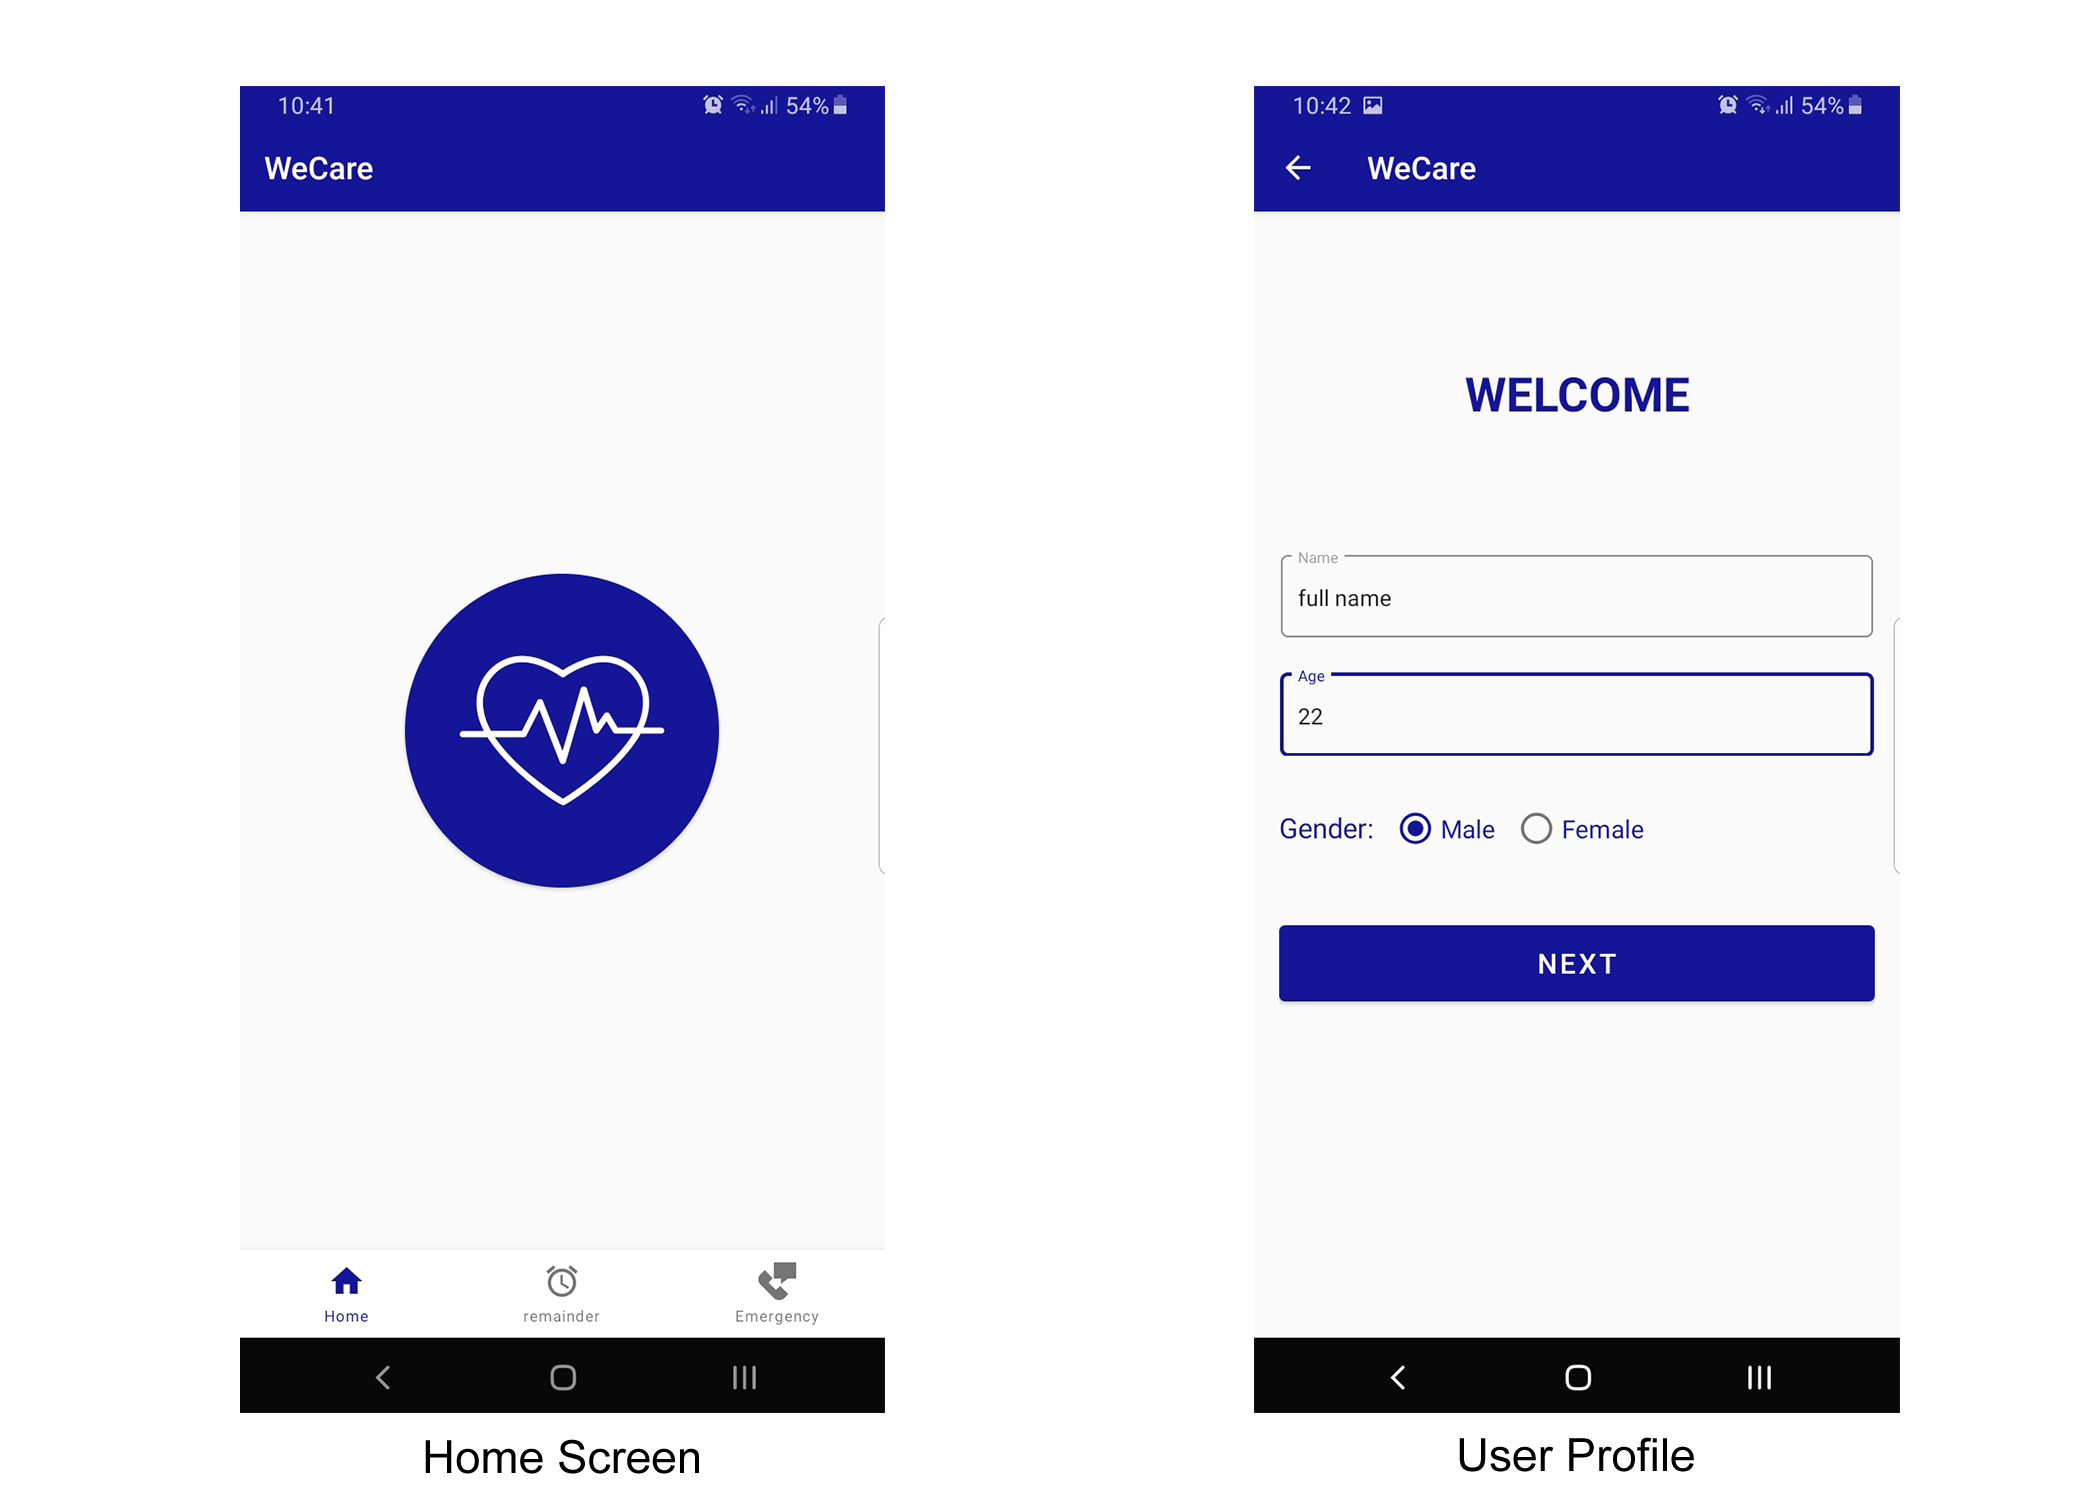
\includegraphics[width=155mm, height = 140mm]{Outputnew/1.png}
\caption{Home Screen and User Profile Screen}
\end{center}
\end{figure}

Home Screen is entry point of our application. User Profile is where user inputs their name,age and gender.

\begin{figure}[H]
\begin{center}
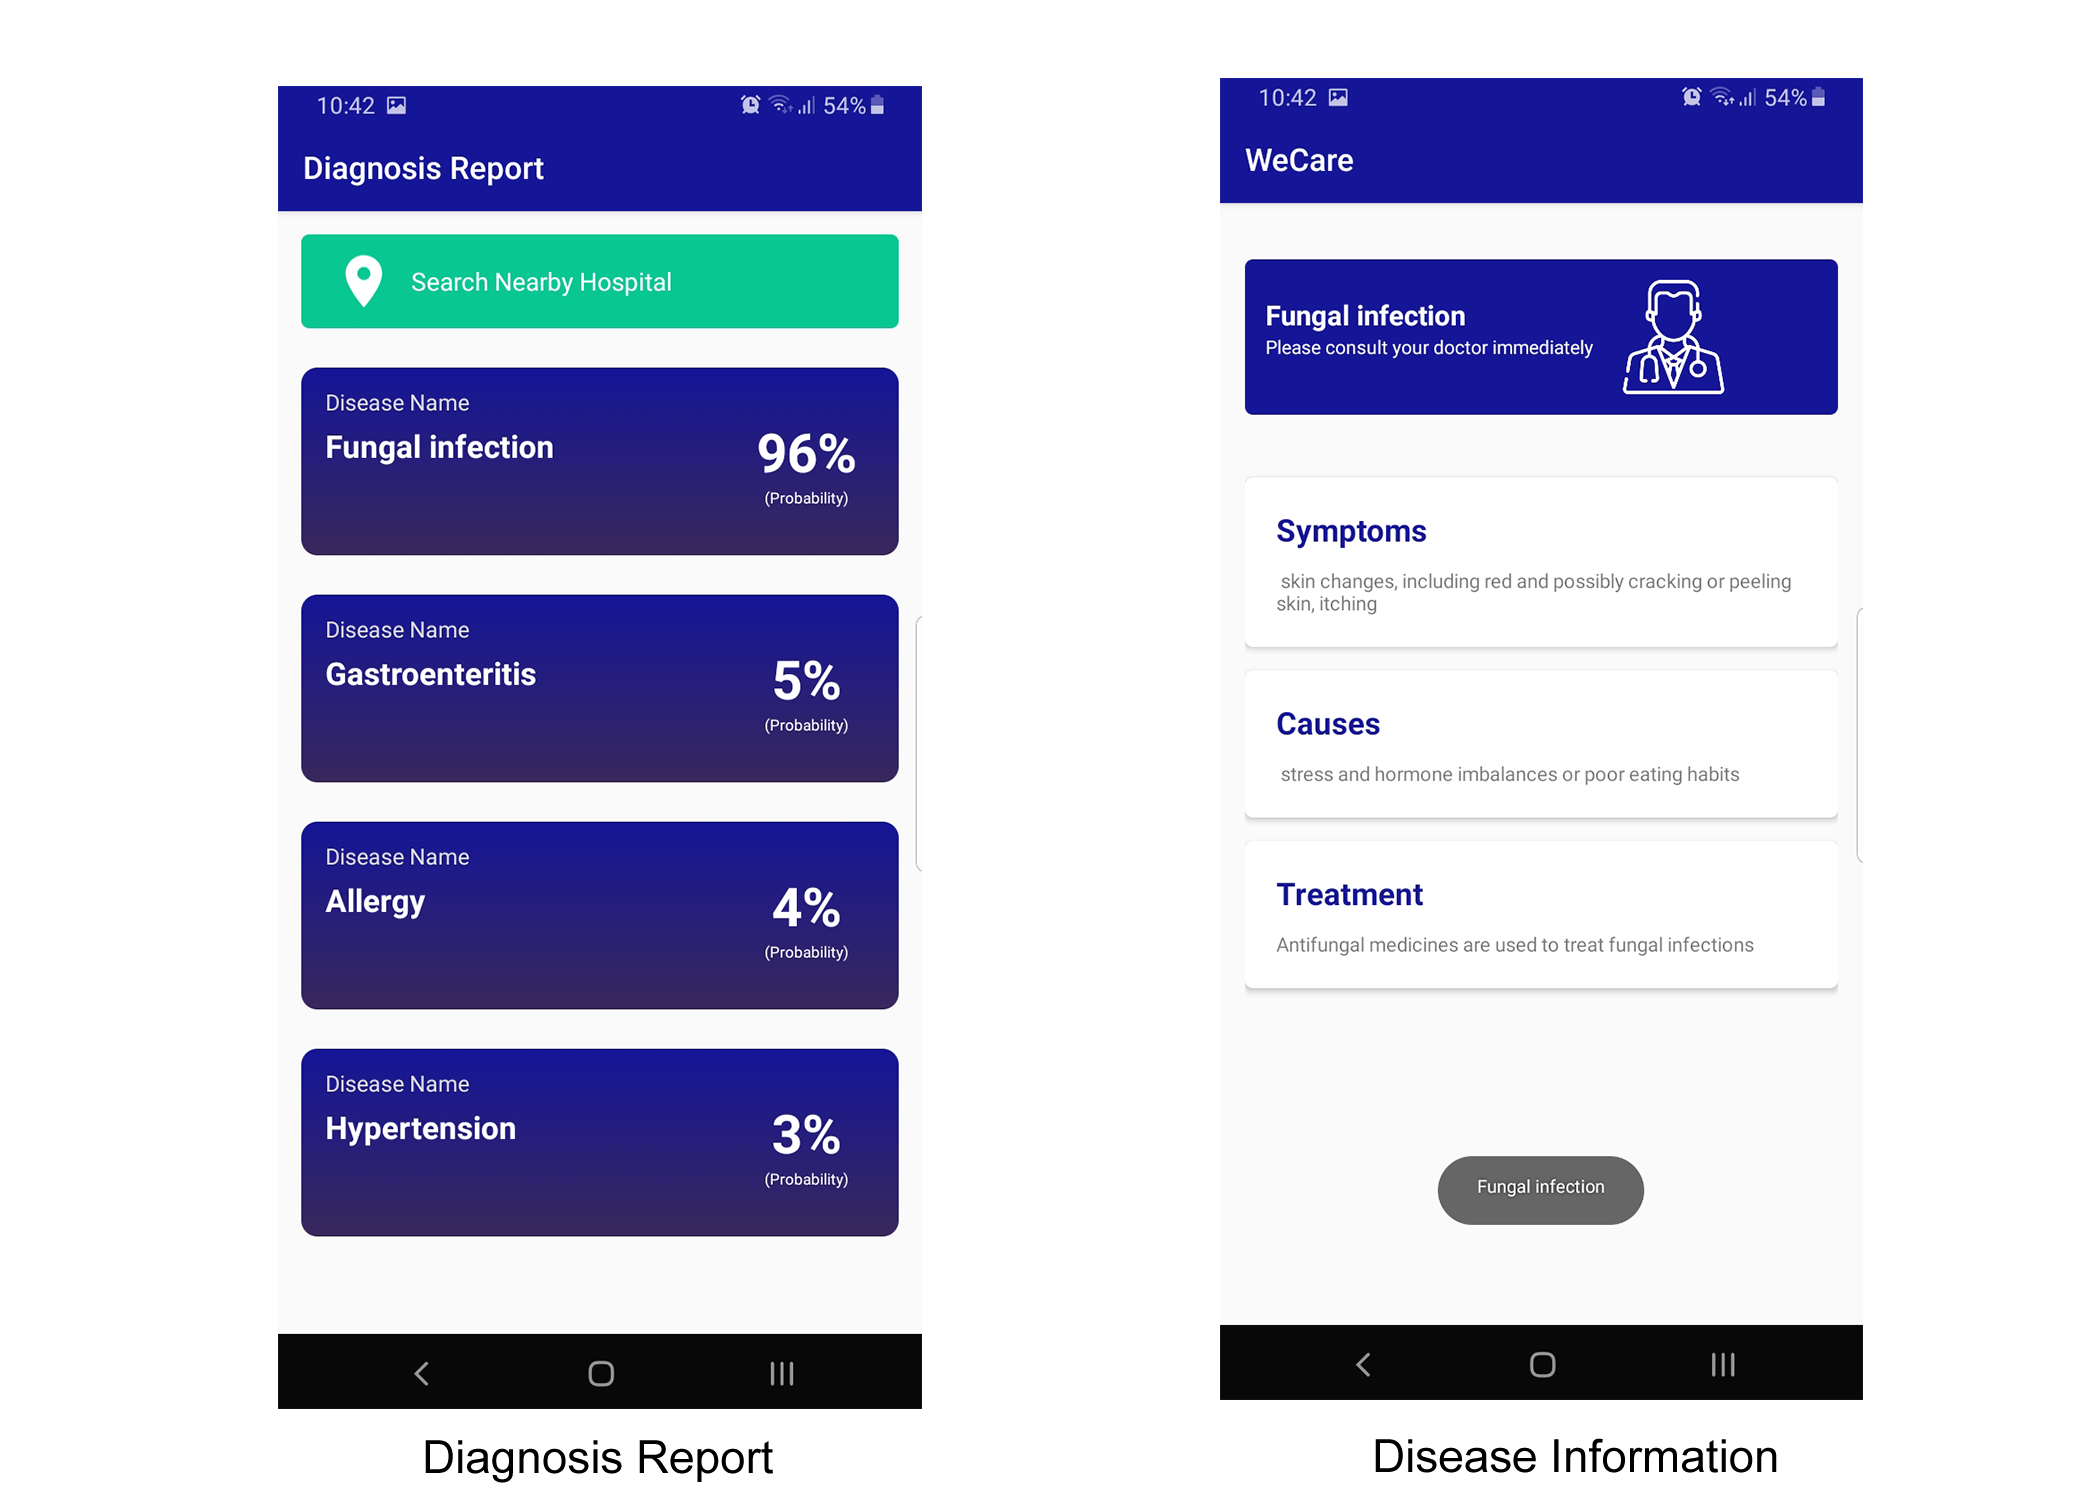
\includegraphics[width=155mm, height = 140mm]{Outputnew/2.png}
\caption{Symptom Input and Diagnosis Report Screen}
\end{center}
\end{figure}

User provide symptoms by selecting from the drop down menu as shown in Selection of Symptoms.Symptoms list is fetch from restful API and after clicking the examine button user symptom is send to the server and got response back from server in Diagnosis Report showing the top 4 probable diseases.Disease information like symptoms,causes and treament are display here.

\begin{figure}[H]
\begin{center}
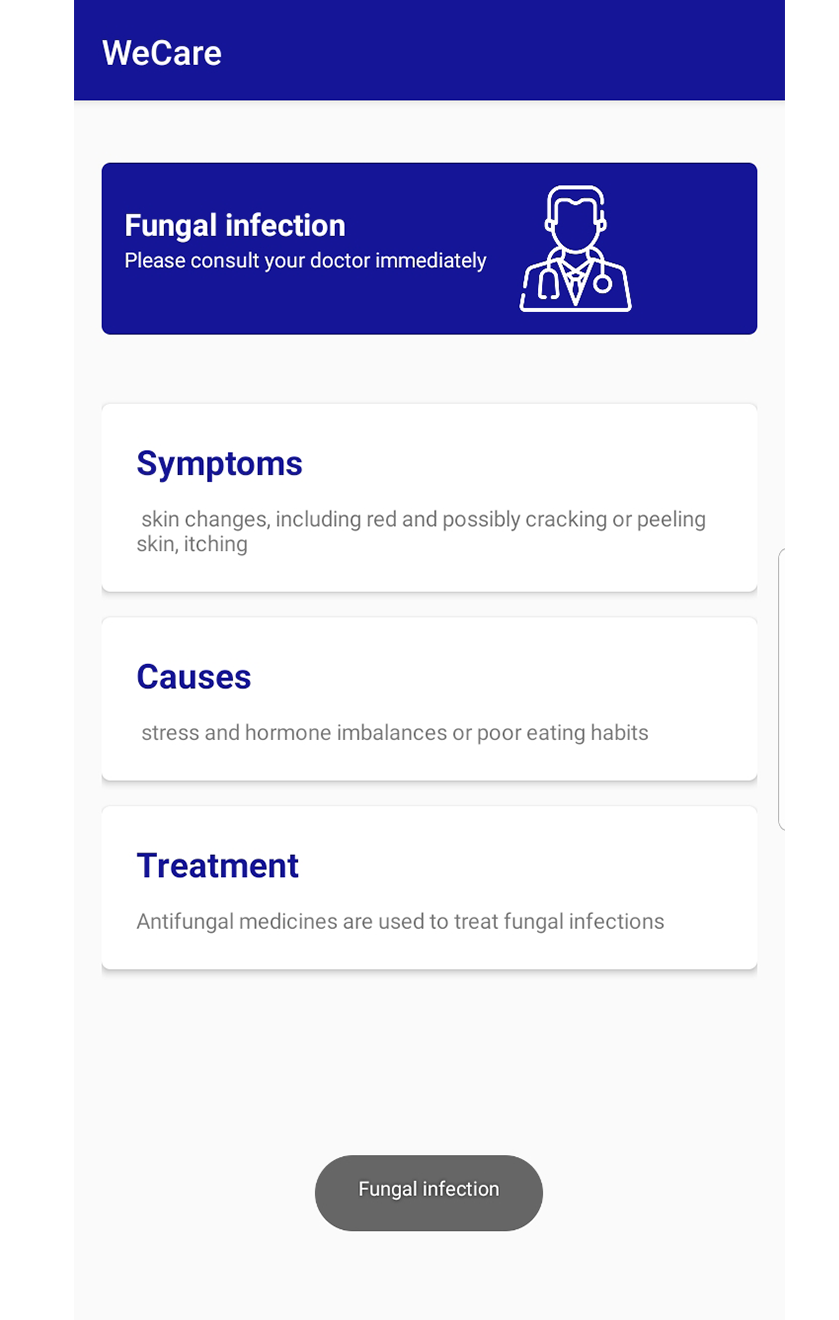
\includegraphics[width=95mm, height = 150mm]{Outputnew/3.png}
\caption{Disease Information}
\end{center}
\end{figure}
Shows Disease Information like symptoms, cause and treatments. 


\begin{figure}[H]
\begin{center}
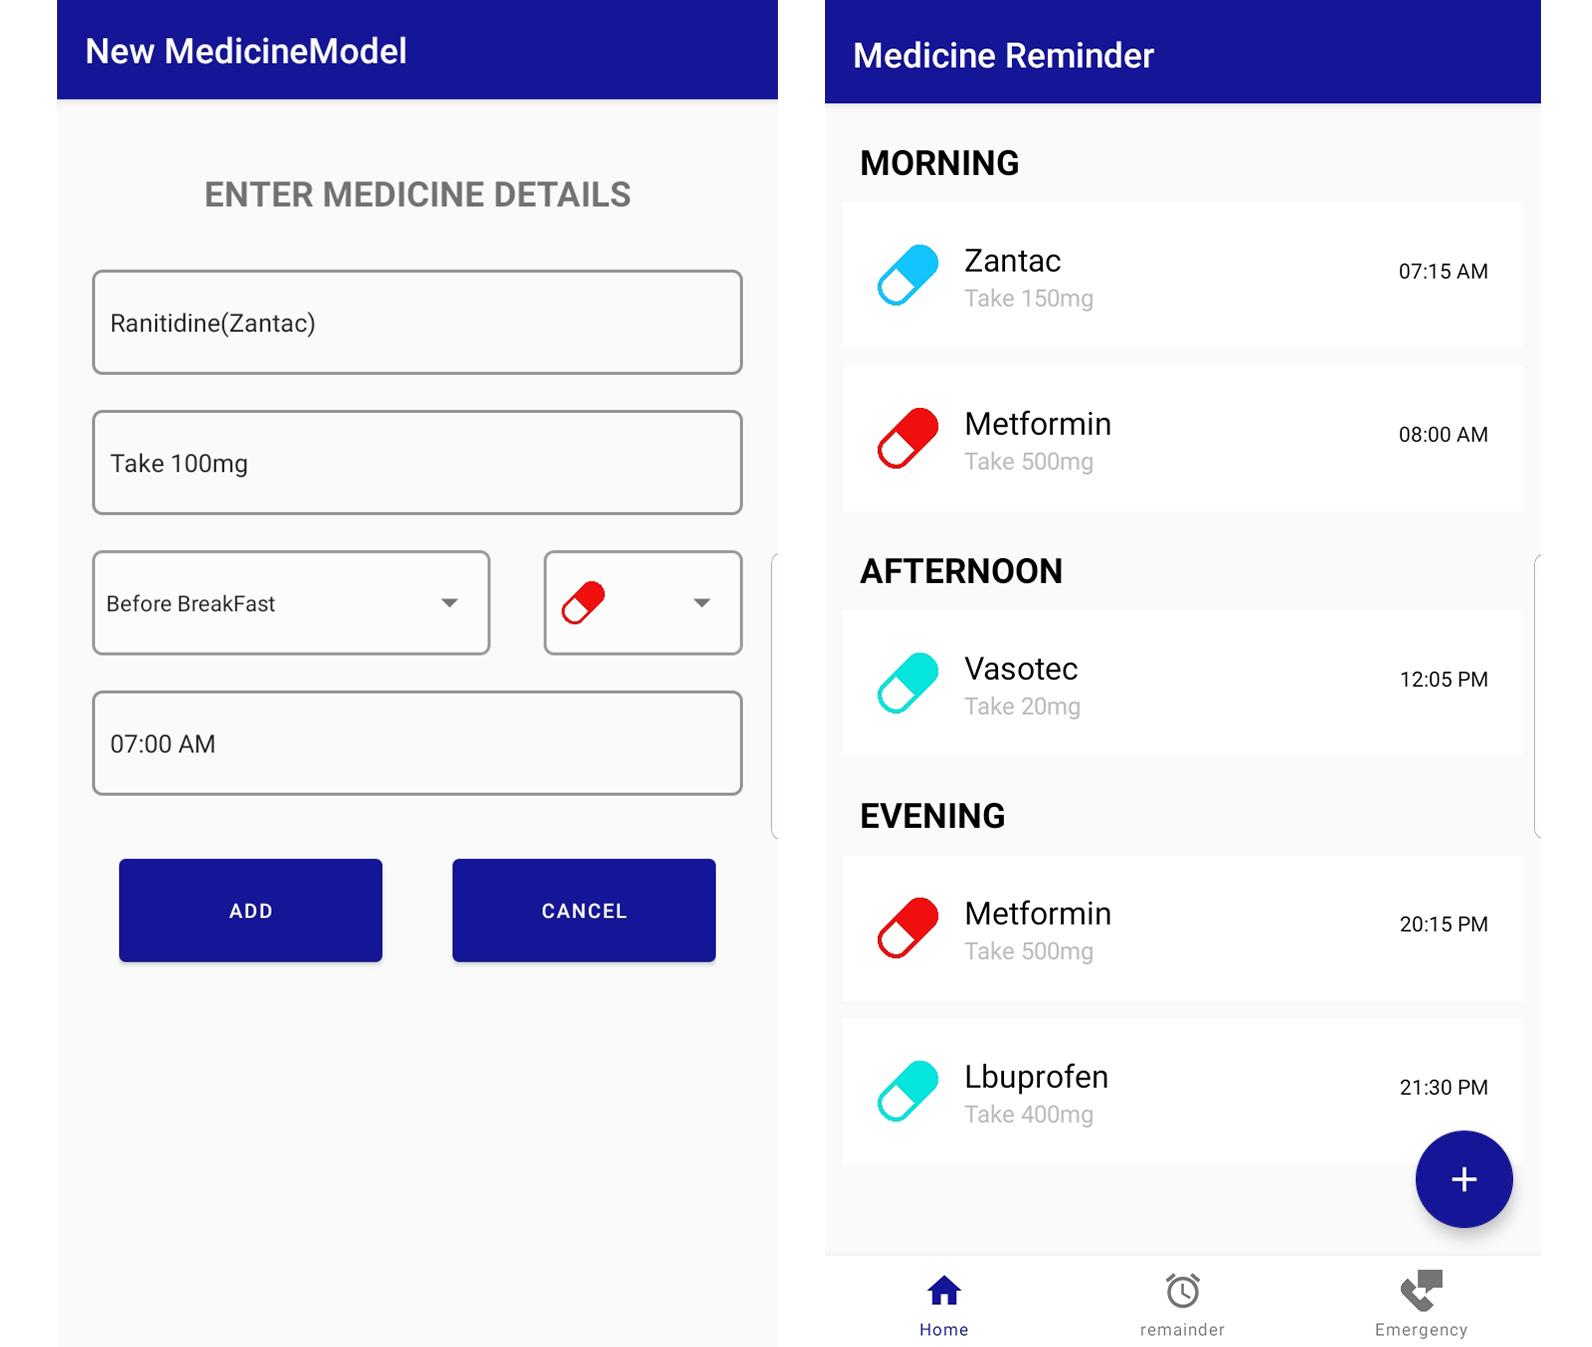
\includegraphics[width=155mm, height = 140mm]{Outputnew/4.png}
\caption{Medicine Reminder Entry and Home Screen}
\end{center}
\end{figure}

Medicine Reminder Entry point where add medicine details like Medicine name,medicine dosage,medicine time. Home screen of pill reminder which shows all entry in pill reminder


\begin{figure}[H]
\begin{center}
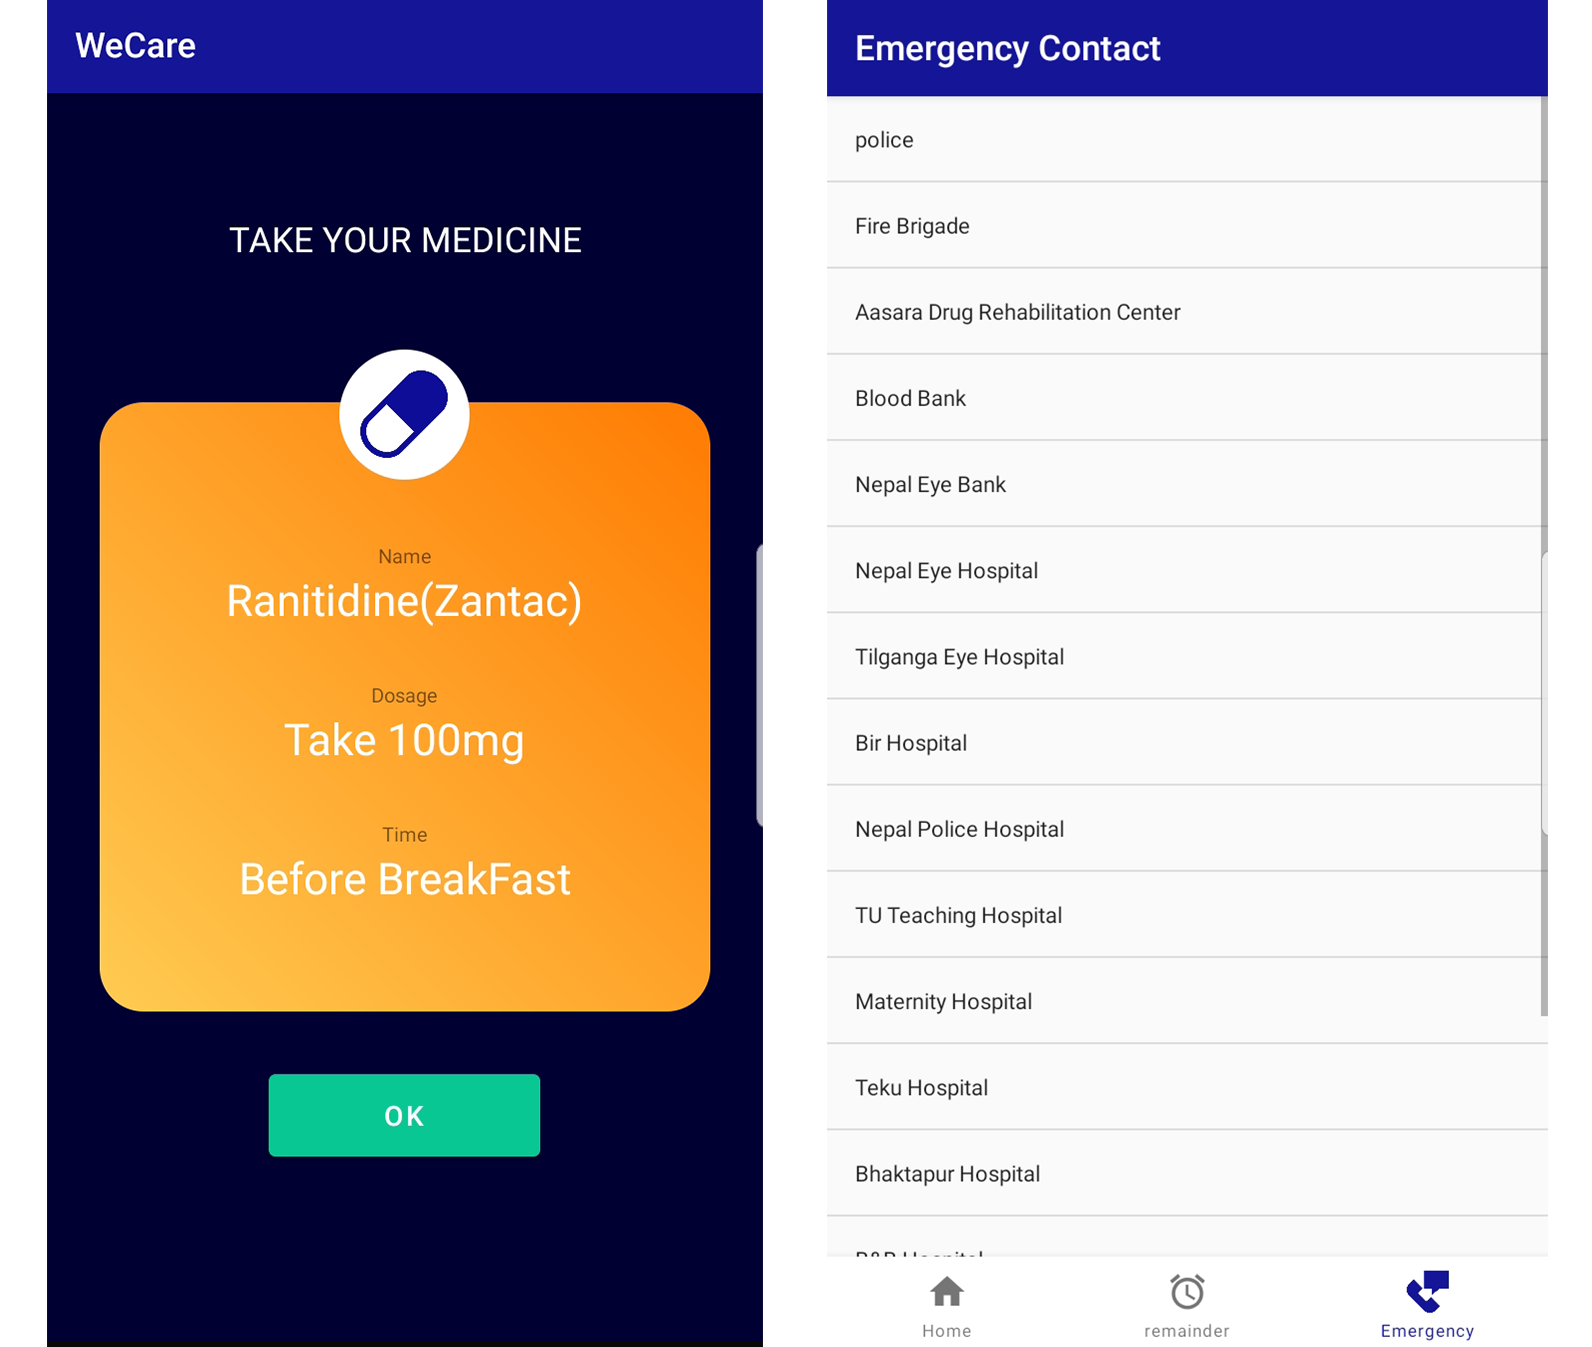
\includegraphics[width=155mm, height = 140mm]{Outputnew/5.png}
\caption{Emergency Contact Screen}
\end{center}
\end{figure}

Medicine reminder alert screen is shown in Medicine Reminder Entry where it shows detail about the medicine name,medicine dosage, and medicine time. Medicine Reminder Home shows the emergency contacts.


\section{Limitations}
In spite of all hardwork, our project consist some limitation. Our project has lack of reliable information. Users cannot describe the detailed information such as if someone is having fever he/she could not describe the temperature and also if someone having pain in any part of the body, how much it is paining. There is only limited number of disease which our project can predict. Users cannot enter their symptoms on their own.\par 
A machine learning model can provide more accurate outcome if the number of hidden layer is increased. But the increase in number of hidden layers leads to computational complexities which cannot be operate by our normal computer. So, we had to use only 5 number of hidden layer. We can use more hidden layer but the complexities and consumption of time will also increases. There is no design guidelines and accuracy depends on training and learning which is not always available. It is hard to maintain degree of meaningfulness and also hard to combine cases together. Predictions are limited to the cases that have been observed. They require accurate details on many past projects. They have large data requirement to learn about various topics which may be time taking and cause various resources.\par 
The actual problem with this inevitable fact is that when they do make errors, diagnosing and correcting them can be difficult because it will require going through the underlying complexities of the algorithms and associated processes. It is impossible to make immediate accurate predictions with a back propagation. It always learns through historical data. The bigger the data and the longer it is exposed to these data, the better it will perform. There is lack of variability. Back propagation deals with statistical truths rather than literal truths. In situations that are not included in the historical data, it will be difficult to prove with complete certainty that the predictions made is suitable in all scenarios. Unlike humans, computers are not good storytellers. Back propagation cannot always provide rational reasons for a particular prediction or decision. They are also limited to answering questions rather than posing them. These systems does not understand context. Depending on the provided data used for training, machine learning is also prone to hidden and unintentional biases. Human input is still important to better evaluate the outputs of these systems.

\section{Challenges}
During our project, we have faced some challenges which has been overcome. Those challenges are explained below:
\begin{itemize}
    \item To train a machine learning model, we need large training datasets so that the prediction could be more accurate. It required time to collect a sufficient amount of data. Collecting appropriate data was most difficult task. Hospitals or any Health Organization may unwilling to share their dataset with us or may issue a formal complaint against us if when they realize that we have use their dataset. Even after collecting the appropriate data, there are also problems of a different nature like preparing data for algorithm training is a complicated process.
    \item  For our project, we have to be familiarize with many software like: 
    \begin{itemize}
        \item Pycharm
        \item Juypter NoteBook 
        \item Visual Studio Code 
        \item Android Studio
    \end{itemize}
     Due to limited knowledge about software, we find very hard to get start with the project. Since our project is based on machine learning, Machine learning comes with a set of predefined recipes called algorithms that are best suited for solving a particular problem.
For example, choosing between K-Nearest Neighbor algorithm, Naive Bayes Algorithm, Random forest algorithm, Decision Tree Algorithm and Back Propagation Algorithm can be confusing to a beginner. Like most of the branches in computer science, ML offers multiple techniques to solve the same problem. So, we have to use different evalution techniques for selection of optimal machine learning algorithm for our project. After day-by-day using those softwares, we understood and familiarize with those software and able to the get appropriate results.  
    \item  We also find difficult to choose optimal algorithm for prediction and hyperparameter for training of Neural Network. We have used 4 different algorithms which are: Naive Bayes Algorithm, Random forest algorithm, Decision Tree Algorithm and Back Propagation Algorithm to train our Neural Network. After using these algorithms for training, we have noted the final outcome of each algorithms. Among those algorithms, Back Propagation Algorithm shows the best result. So, we carried our project with Back Propagation Algorithm.
\end{itemize}

\section{Work Schedule}
\begin{figure}[H]
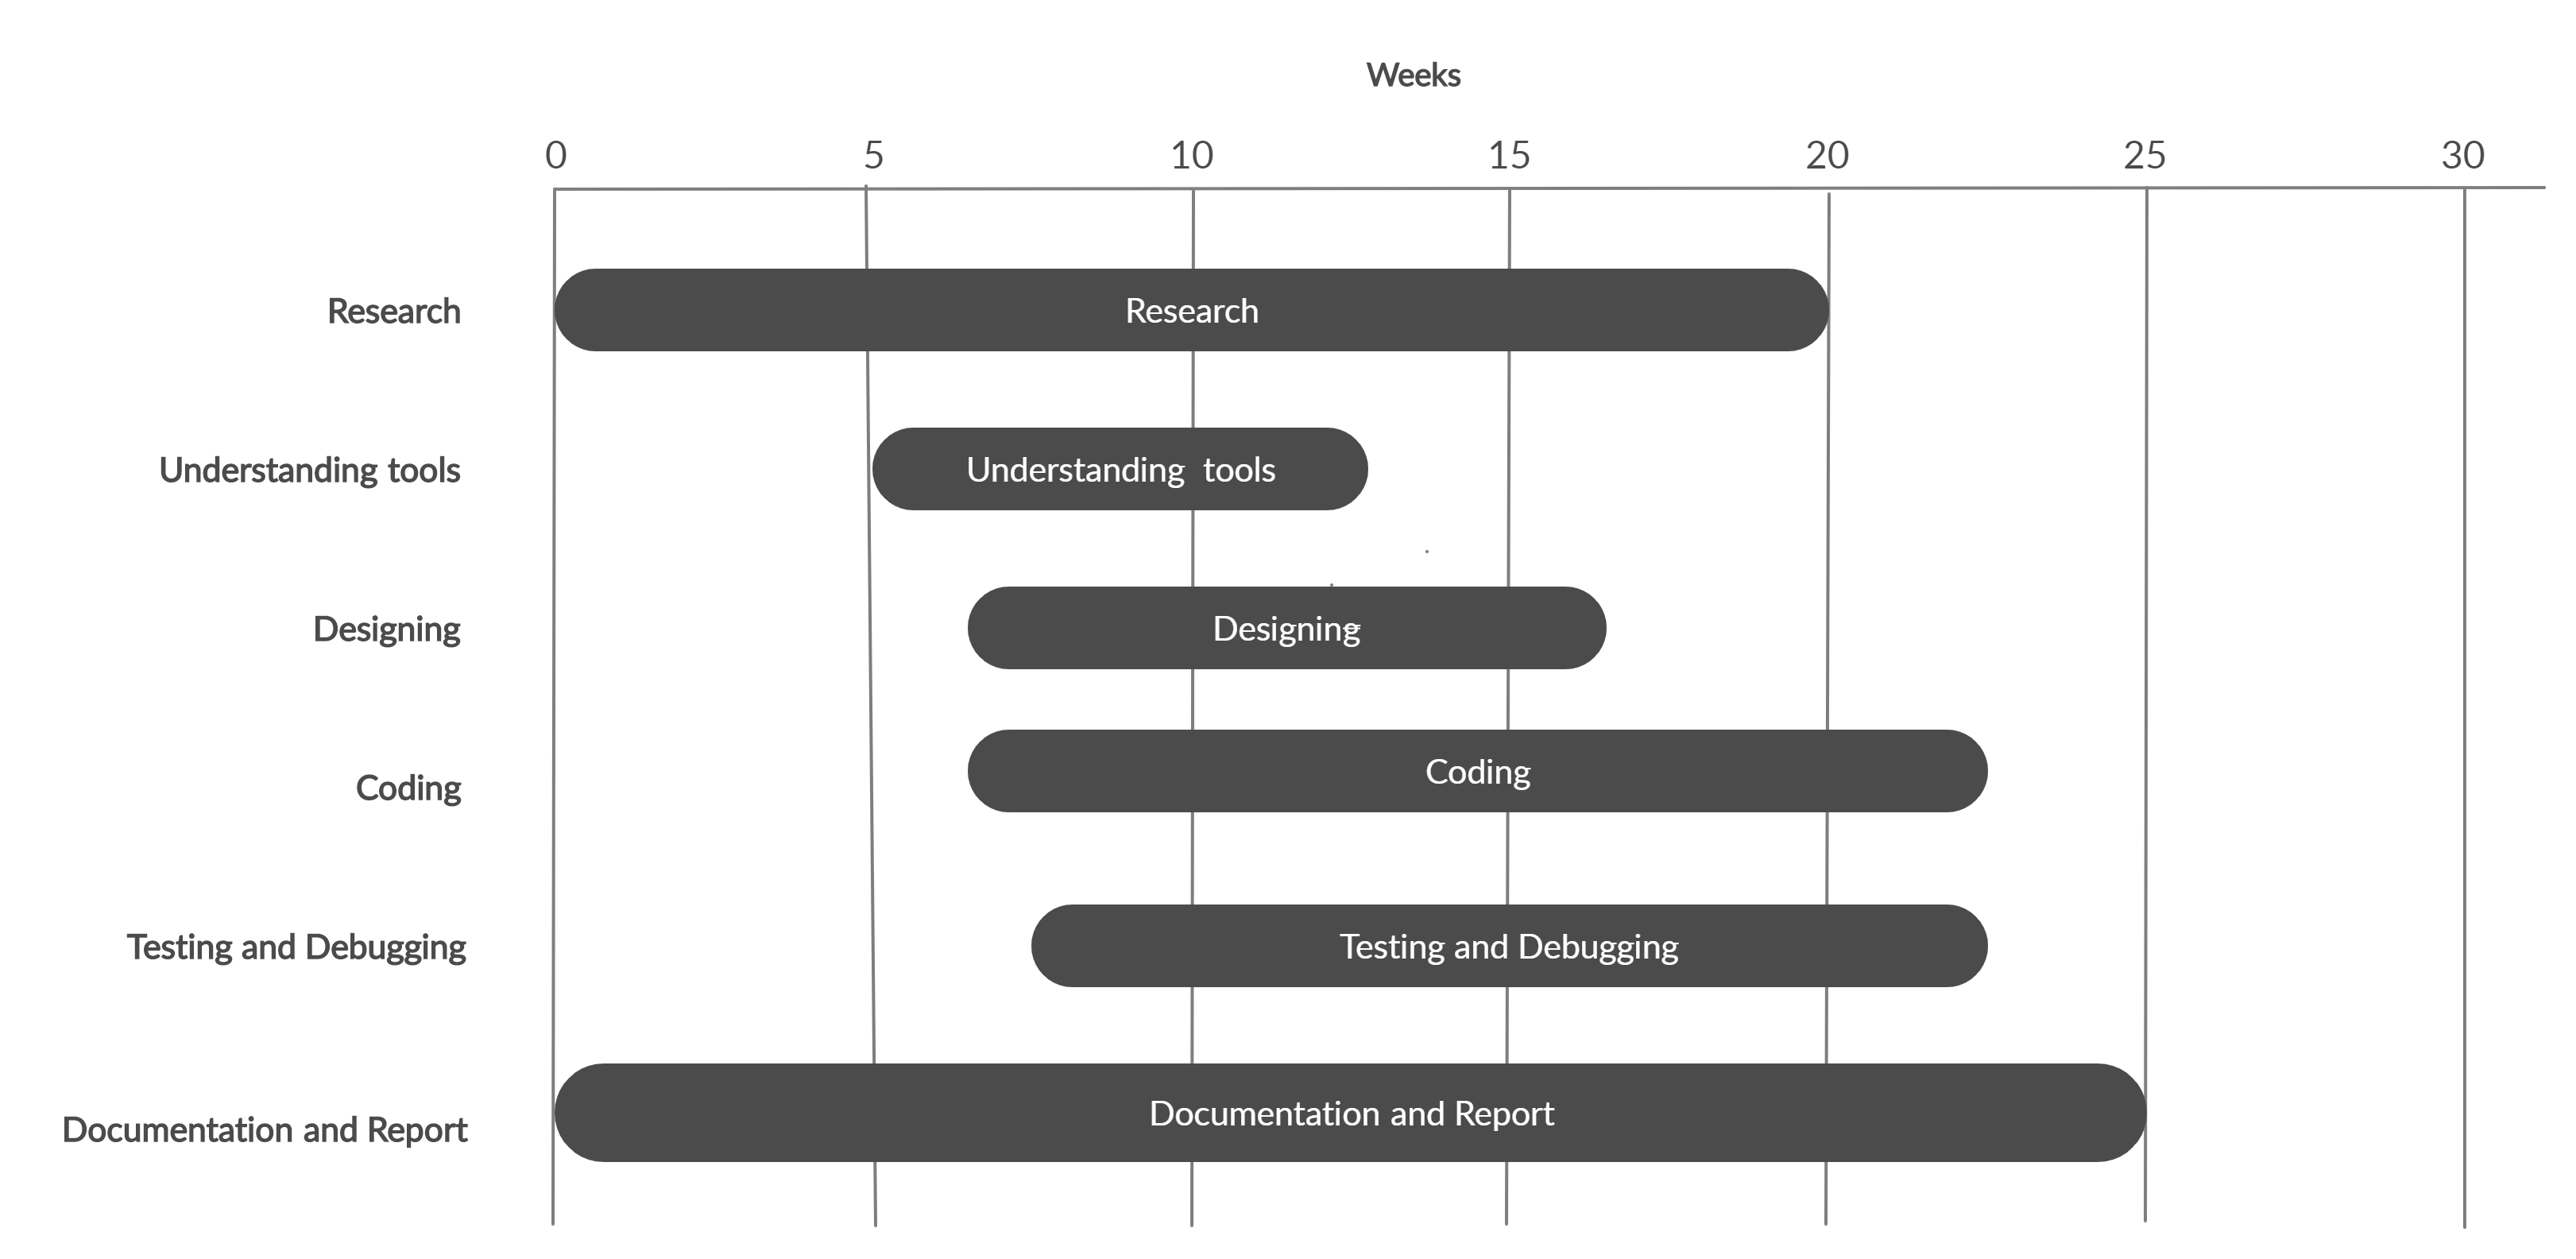
\includegraphics[width=150mm,height=90mm]{images/ganttchartnew.jpg}
 \caption{Gantt Chart}
\end{figure}

\section{Future Enhancements}

For now our project is capable of only determining/predicting diseases according to provided
symptoms only. The same architecture could be extended to predict other diseases as well
after analysing the various symptoms of those diseases in consultation with the concerned 
health experts. 

Our project has got a lot of potential; for now due to limitation to our knowledge and time, we have proposed an able system to predict provided diseases only.

In future additional extra features can be added such as;- 
\begin{itemize}
    \item Natural Language Processing:In future natural language processing can be used in our project which allow user to provide symptoms in english language rather then selecting symptoms from drop down menu
    \item SMS Based:In future SMS based system can be implement in our system which allow user at remote area of nepal to get access to our system and also it doesn't require high bandwidth connection and smartphone.
   
   \item Near By Hospital: We can also implement google map api to get information about the nearest hospital from user location
        
\end{itemize}

\section{Conclusion}
 
Our project system is on disease prediction and we have created an android app 
which can be access by anyone, through with the use of internet. Our system take 
symptoms as input, processes them and provide provisional diagnosed diseases as 
results to users. It is a two click output method; which makes it simple and ease to use. 
Our system also provides feature of pill reminder which can work as an important function 
regarding the people where age is also a factor.\par

Our proposed system of disease prediction with appropriate diagnosis has been framed
up using Artificial Neural Network. For effective prediction, we trained various models;
back propagation ANN, decision tree, random forest and compare the parameters iteratively. 
The various models algorithm has been repeated until minimun error rates were observed 
on them. It is proven from the results that the proposed method, back propagation artificial 
neural network effectively predicts accuracy around 95.42\% and hence. Chosen as an optimal algorthim for our project.\par

Also in neural network its various parameter were adjusted from time to time to give 
the better results. The number of hidden layers and tuning the hyperparameters like
learning rate, epoch etc for increasing the performance model for our project is still in 
working stage.





\chapter*{References}

[1] Shreevastava M. And Gupta A. (2011) “ Medical Diagnosis using Back Propagation Algorithm”, International Journal of Emerging Technology and advanced Engineering, ISSN 2250-2459, Vol. 1, Issue 1, November 2011.\par
[2] Taufik, Wan & Ab Ghani, Nur Laila & Mohd Drus, Sulfeeza. (2019). Data Mining Techniques for Disease Risk Prediction Model: A Systematic Literature Review: Proceedings of the 3rd International Conference of Reliable Information and Communication Technology (IRICT 2018). 10.1007/978-3-319-99007-1_4. \par
[3] Kadhim Qeethara (2011), “Artificial Neural Networks in Medical Diagnosis”. International Journal of Computer Science, Vol. 8, Issue 2, March 2011  \par
[4] Sumathi B., Santhakumaran A. (2011), “Pre-Diagnosis of Hypertension using Artificial Neural Network”, Global Journal of Computer Science and Technology, Vol. 11, issue 2, version 1.0, February 2011.\par
[5] Al-Shayea, Qeethara. (2011). Artificial Neural Networks in Medical Diagnosis. Int J Comput Sci Issues. 8. 150-154.\par
[6] Escobar GJ, Turk BJ, Ragins A, et al. Piloting electronic medical record-based early detection of inpatient deterioration in community hospitals. J Hosp Med. 2016;11(1):S18–S24.\par
[7] Dilip  Roy  Chowdhury,  Mridula  Chatterjee  R.K. Samanta, An  Artificial Neural Network Model for Neonatal Disease Diagnosis, International  Journal of Artificial Intelligence  and Expert Systems (IJAE), Volume (2): Issue(3),2011.\par
[8] Milan  Kumari,  Sunila  Godara,  Comparative  Study  of  Data  Mining  Classification  Methods  in  Cardiovascular  Disease  Prediction,  IJCST  Vol. (2), Issue (2), June 2011.\par
[9] Vanisree  K, Jyothi Singaraju, Decision Support System for Congenital Heart Disease Diagnosis based on Signs and Symptoms using Neural   Networks, International  Journal of   Computer Applications (0975 8887) Volume 19 No.6, April 2011.\par
[10] Niti Guru, Anil Dahiya, Navin Rajpal, Decision Support System for Disease Diagnosis    Using Neural Network, Delhi Business Review, Vol.8, No.1, January-June 2007.\par
[11] Sellappan Palaniappan, Rafiah Awang, Intelligent Heart Disease Prediction System Using  Data Mining Technique, 978-1-4244-1968-5/08/, 2008 IEEE.\par
[12] Smitha.T,Dr.V.Sundaram”Classification Rules By DecisionTree for disease Prediction”, ,International journal of Computer Applications vol-43, No-8, April 2012.\par





\end{document}
